\documentclass{article}
\usepackage{ifpdf}
\usepackage[noshading,chorded]{songs}
\usepackage[utf8]{inputenc}
% \usepackage[nf]{coelacanth}
% \usepackage[default,regular]{sourceserifpro}
% \usepackage{venturis2}
% \usepackage{fourier}
% \usepackage{Alegreya}
% \renewcommand*\oldstylenums[1]{{\AlegreyaOsF #1}}
% \usepackage{caladea}
% \usepackage[bitstream-charter]{mathdesign}
% \usepackage[light]{CrimsonPro}
% \usepackage[medium]{CrimsonPro}
% \usepackage{paratype} 
\usepackage{stickstootext}
\usepackage[T1]{fontenc}
%% The font package uses mweights.sty which has som issues with the
%% \normalfont command. The following two lines fixes this issue.
% \let\oldnormalfont\normalfont
% \def\normalfont{\oldnormalfont\mdseries}
\usepackage{pdfpages}
\usepackage{hyperref}
\usepackage{cclicenses}

\usepackage[a4paper, margin={1in}]{geometry}

%% The font package uses mweights.sty which has som issues with the
%% \normalfont command. The following two lines fixes this issue.
\let\oldnormalfont\normalfont
\def\normalfont{\oldnormalfont\mdseries}
\noversenumbers
\nosongnumbers
% \songcolumns{1}
% \spenalty=-10000
% \afterpreludeskip=2pt plus 1fil
% \beforepostludeskip=2pt plus 1fil

\setlength{\sbarheight}{0pt}
% \pagenumbering{gobble}


\pagestyle{plain}

\renewcommand{\flatsymbol}{m}

% \renewcommand{\lyricfont}{\large}
\renewcommand{\printchord}[1]{\rmfamily\bf#1}
\renewcommand{\idxauthfont}{\large\it}
\renewcommand{\stitlefont}{
  \rmfamily\bf\huge\baselineskip=20pt\lineskiplimit=0pt
}

\notenames{A}{H}{C}{D}{E}{F}{G}

\def\refchorus{
\beginverse
\vspace{-0.15in}
\hspace{0.25in}\textbf{Ref.}
\vspace{-0.05in}
\endverse
}

\renewcommand{\songtarget}[2]
{\pdfbookmark[#1]{\thesongnum. \songtitle}{#2}}
\renewcommand{\songlink}[2]{\hyperlink{#1}{#2}}

\renewcommand{\songchapter}{\chapter*}
\renewcommand{\songsection}{\section*}
\renewcommand{\idxrefsfont}{\bfseries}

\renewcommand{\idxtitlefont}{\rmfamily}
% \renewcommand{\idxlyricfont}{\rmfamily\mdseries}

\renewcommand{\idxheadfont}{\bfseries\rmfamily}
\setlength{\idxheadwidth}{0cm}

\def\caponote[#1]{
\hspace{-0.66cm}\textit{(capo #1)}
}

\def\chordskip{
  \vspace{-0.5cm}
}

% \newindex{mainindex}{idxfile}

\usepackage{xpatch}

\makeatletter
\xpatchcmd{\SB@@@beginsong}
  {\SB@addtoindexes\songtitle}
  {\SB@addtoindexes{\songtitle\ifx\songauthors\empty\else\ -- \songauthors\fi}}
  {}{}
\makeatother

\sepindexesfalse

\newindex{idx1czech}{toc/idx1czech}
\newindex{idx1international}{toc/idx1international}
\newindex{idx2czech}{toc/idx2czech}
\newindex{idx2international}{toc/idx2international}
\indexsongsas{idx1czech}{\thepage}
\indexsongsas{idx1international}{\thepage}

\begin{document}

\pagenumbering{gobble}
% 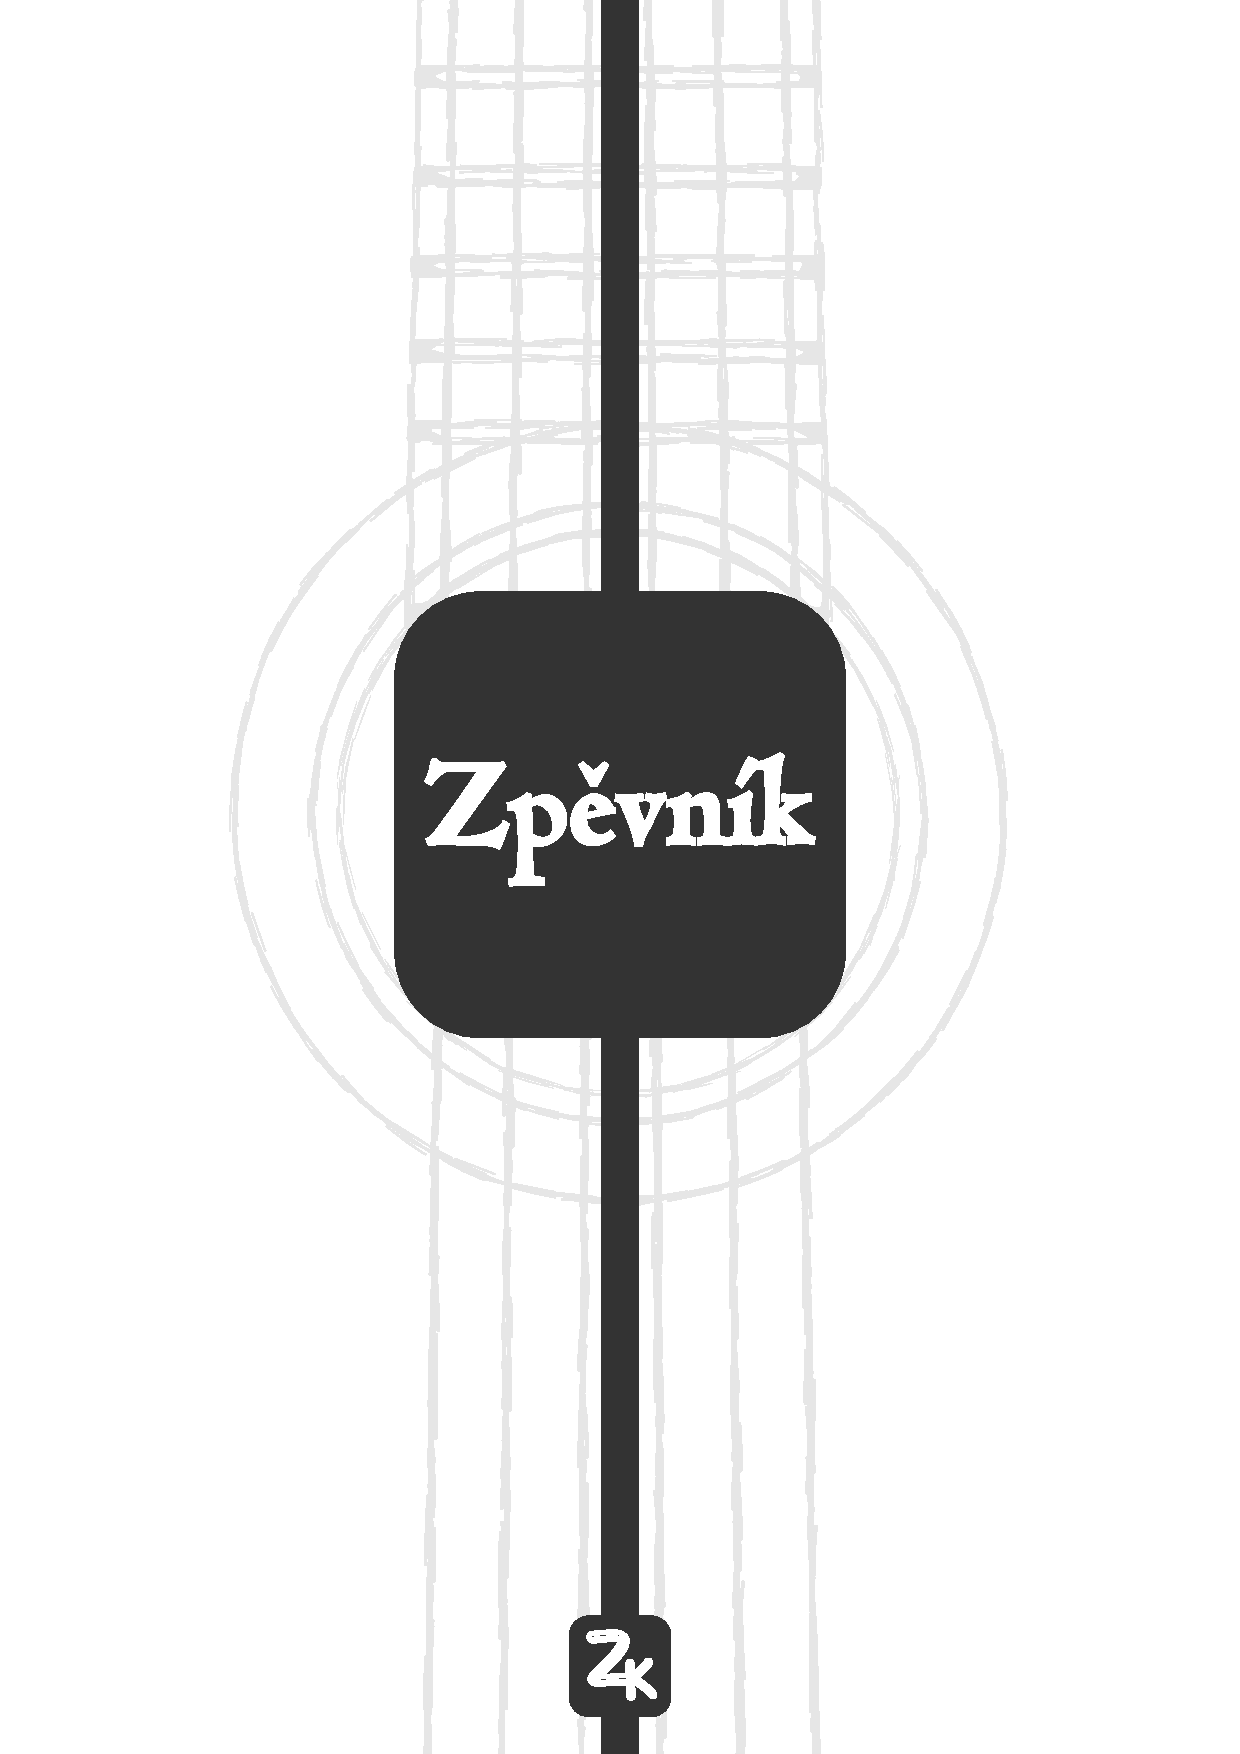
\includepdf[pages=-]{cover/cover.pdf}

% \vspace*{\fill}
% \begin{center}
%   \Huge\bfseries X-Challenge zpěvník
% \end{center}
% \vspace*{\fill}

\pagebreak
\showindex[2]{\huge České a slovenské}{idx1czech}
\newpage
\showindex[2]{\huge Zahraniční}{idx1international}
% \vspace{1cm}
\pagenumbering{arabic}
\leavevmode\thispagestyle{empty} \newpage

\leavevmode\thispagestyle{empty} \newpage
\vspace*{\fill}
\begin{center}
  \Huge\bfseries České a slovenské
\end{center}
\vspace*{\fill}
\pagebreak

\begin{songs}{idx1czech}
  \beginsong{Amerika}[by={\normalsize Lucie}]
\beginverse
\[G]Nandej mi \[D]do hlavy tvý \[A&]brouky
A Bůh nám seber bezna\[G]děj
V duši zbylo \[D]světlo z jedný \[A&]holky
Tak mi teď za to vyna\[G]dej
\endverse

\beginverse
\[G]Zima a pro\[D]marněný \[A&]touhy
Do vrásek stromů padá \[G]déšť
Zbejvaj roky \[D]asi ne moc \[A&]dlouhý
Do vlasů mi zabro\[C]ukej... pa pa pa \[G]pá
\endverse

\beginchorus
\[G]pa pa \[G/F#]{pa pá},\[E&] pá pa pa pá\[G]
\[G]pa pa \[G/F#]{pa pá},\[E&] pá pa pa pá\[G]
\endchorus

\beginverse
\[G]Tvoje oči \[D]jenom žhavý t\[A&]óny
Dotek slunce zapa\[G]dá
Horkej vítr \[D]rozezní mý z\[A&]vony
Do vlasů ti zabro\[C]ukám ... pá pa pá \[G]pá
\endverse

\refchorus \rep{2}

\beginverse
\[G]Na obloze \[D]křídla tažnejch \[A&]ptáků
Tak už na svý bráchy zavo\[G]lej
Na tváře ti p\[D]adaj slzy z mr\[A&]aků
A Bůh nám sebral bezna\[G]děj
\endverse

\beginverse
\[G]V duši zbylo \[D]světlo z jedný \[A&]holky
Do vrásek stromů padá \[G]déšť
Poslední dny \[D]hodiny a \[A&]roky
Do vlasů ti zabrou\[C]kám... pá pa pá \[G]pá
\endverse
\refchorus

\endsong
  \beginsong{Anděl}[by={\normalsize Karel Kryl}]

\transpose{5}
\preferflats

\beginverse
\[G]Z rozmláce\[E&]nýho kostela \[G]v krabici \[D7]s kusem mýdla,
\[G]přinesl \[E&]jsem si anděla, \[G]poláma\[D7]li mu křídla. \[G]
\[G]Díval se \[E&]na mě oddaně, \[G]já měl jsem \[D7]trochu trému.
\[G]Tak vtiskl \[E&]jsem mu do dlaně \[G]lahvičku \[D7]od parfému. \[G]
\endverse
\beginchorus
\[G]A proto \[E&]prosím, věř mi, \[G]chtěl jsem ho \[D7]žádat,
\[G]aby mi \[E&]mezi dveřmi \[G]pomohl \[D7]hádat,
\[G]co mě čeká\[E&] \[D7]a nemi\[G]ne,
\[G]co mě čeká\[E&] \[D7]a nemine.\[G]
\endchorus
\beginverse
^Pak hlída^{li jsme} oblohu ^pozoru^jíce ptáky,
^debatu^jíce o Bohu ^{a hraní} ^na vojáky. ^
^Do tváře ^jsem mu neviděl ^pokoušel ^se ji schovat,
^to asi ^ptákům záviděl, ^že mohou ^poletovat. ^
\endverse

\refchorus

\beginverse
^Když novin^ky mi sděloval ^u okna ^do ložnice,
^já křídla ^jsem mu ukoval ^z mosazný ^nábojnice. ^
^A tak jsem ^pozbyl anděla, ^on oknem ^uletěl mi,
^však přítel ^prý mi udělá ^novýho ^z mojí helmy. ^
\endverse

\refchorus

\endsong

  \beginsong{Andělé}[by={\normalsize Wanastowi vjecy}]
\beginverse
\[H]Co tě to h\[C#&]ned po ránu n\[E]apadá
\[H]Nohy ruce \[C#&]komu je chceš d\[E]át
\[H]Je to v krvi \[C#&]co tvou hlavu př\[E]epadá
\[H]Chtělas padnout \[C#&]do hrobu a sp\[E]át
\endverse

\beginchorus
\[D]Poranění a\[A]ndělé jdou d\[G]o polí
\[D]Stěhovaví l\[A]idi ulít\[G]aj
\[D]Panenku b\[A]odni - ji to n\[G]ebolí
\[D]Svět je mami p\[A]rapodivnej k\[G]raj
\endchorus

\beginverse
\[H]Po ránu p\[C#&]rincezna je os\[E]palá
\[H]Na nebi \[C#&]nemusí se bá\[E]t
\[H]V ulicích \[C#&]doba zlá ji sp\[E]outala
\[H]Polykač n\[C#&]álezů a ztr\[E]át
\endverse

\refchorus

\beginverse
\[H]Co tě to \[C#&]zas po ránu n\[E]apadá
\[H]Za zrcadlem \[C#&]nezkoušej si l\[E]hát
\[H]Miluju tě, ch\[C#&]ci tě - to ti př\[E]ísahám
\[H]Na kolenou \[C#&]lásce pomož vs\[E]tát
\endverse

\refchorus (\ldots dokonalej kraj)

\beginverse
\[D]Svět je mami d\[A]okonalej k\[G]raj \rep{4}
\endverse
\endsong
  \beginsong{Ani k stáru}[by={\normalsize Zdeněk Svěrák}]
\beginverse
\[C]Mám ploché nohy po tetě a fanta\[F]zii po svém strýci,
už dlouho \[A&]šlapu po světě, a nevím \[G]co mám o něm říci.
Kdysi jsem \[C]sníval o Nilu a pak se \[F]plavil po Vltavě,
já věřil \[A&]spoustě omylů a dodnes \[G]nemám jasno v hlavě,
nemám jasno \[C]v hlavě.
\endverse

\beginchorus
\[C]Ani k stáru, ani k stáru, ani k stáru,
nemám o \[G&]životě páru, nemám páru,
\[F]třeba že jsem \[E&]dosti sečtě\[C]lý, sečtě\[G]lý.
Až mi \[C]tváře zcela zblednou zcela zblednou,
dal bych \[G&]si ho ještě jednou, ještě jednou,
třeba s \[F]vámi, třeba \[E&]s vámi, chcete-\[C]li.\[C7]
Třeba s \[F]vámi, třeba \[E&]s vámi, chcete-\[C]li.
\endchorus

\beginverse
Už dlouho \[C]šlapu po světě a čekám \[F]co se ještě stane,
mám pořád \[A&]duši dítěte a říka\[G]jí mi starý pane,
já cito\[C]vě jsem založen, při smutných \[F]filmech slzy roním,
a měl jsem \[A&]taky málo žen, teď už to \[G]asi nedohoním.
Už to nedo\[C]honím.
\endverse

\beginchorus
\[C]Ani k stáru, ani k stáru, ani k stáru,
nemám \[G&]o životě páru, nemám páru,
\[F]třeba že jsem \[E&]dosti sečtě\[C]lý, sečtě\[G]lý.
Až mi\[C] tváře zcela zblednou zcela zblednou,
dal bych \[G&]si ho ještě jednou, ještě jednou,
třeba s \[F]vámi, třeba \[E&]s vámi, chcete-\[C]li.\[C7]
Třeba s \[F]vámi, milé d\[G]ámy, chcete-l\[C]i.
\endchorus
\endsong
  \beginsong{Bára}[by={\normalsize Kabát}]

\caponote[2]
\beginverse
\[F#&]Jenom se \[H&]ptej,
kolem \[D]plameny tančí
tak \[A]proč je tady divnej \[G]chlad.
\endverse

\beginverse
\[F#&] Nepospíchej\[H&]
kdo tě \[D]zavede zpátky
a \[A]kdo při tobě bude \[G]stát. Víš já\ldots
\endverse

\beginchorus
Víš já \[D]mám spoustu \[F#&]známejch v pod\[H&]zemí,
a divá \[G]Bára se mnou \[D]spí.
Když je \[D]noc všechno krás\[F#&]ný zdá se \[H&]mi,
to jsme my \[G]dávno prokle\[F#&]tý.
\endchorus

\beginverse
\[F#&] Ještě je čas,\[H&]
jak tě \[D]nestvůra kouše
tak \[A]schovej nohy do pe\[G]řin.
\endverse

\beginverse
\[F#&] Okolo nás\[H&]
je toho \[D]tolik co zkoušet
na \[A]jedno zdraví nev\[G]ěřit. Víš já\ldots
\endverse

\refchorus

\beginverse
\[F#&] Kdopak tě zval,\[H&]
vem si \[D]do dlaně růži,
\[A]sevři ji a krve \[G]pij.
\endverse

\beginverse
\[F#&]Pojď jenom \[H&]dál,
obleč \[D]si moji kůži,
\[A]vysaj mě a pou\[G]žij. Víš já\ldots
\endverse

\refchorus \rep{3}
\endsong
  \beginsong{Básnířka}[by={\normalsize Jaromír Nohavica \& Čechomor}]
\beginverse
\[G]Mladičká \[D]básnířka \[C]s korálky \[D]nad kotní\[G]ky\[D]\[C]\[D]
\[G]bouchala \[D]na dvířka \[C]paláce \[D]poeti\[E&]ky,
s někým se \[C]vyspala \[G]někomu \[C]nedala \[G]láska jako \[D]hobby,
\[G]pak o tom \[D]napsala \[C]sonet na \[D]čtyři do\[G]by.\[D]\[C]\[D]
\endverse

\beginverse
\[G]Své srdce \[D]skloňovala \[C]podle vzoru \[D]Ferlinghe\[G]tti\[D],\[C]\[D]
\[G]ve vzduchu \[D]nechávala \[C]viset vždy jen \[D]půlku vě\[E&]ty,
plná \[C]tragiky\[G], plná \[C]mystiky\[G], plná \[D]splínu,
\[G]tak jí to \[D]otiskli \[C]v jednom \[D]magazí\[G]nu.\[D]\[C]\[D]
\endverse

\beginverse
\[G]Bývala \[D]viděna \[C]v malém baru \[D]u Rozhla\[G]su,\[D]\[C]\[D]
\[G]od sebe \[D]kolena a \[C]cizí ruka \[D]kolem pa\[E&]su,
trochu se \[C]napila\[G], trochu se \[C]opila\[G], na účet \[D]redaktora
\[G]a týden \[D]nato byla \[C]hvězdou \[D]mikrofó\[G]ra.\[D]\[C]\[D]
\endverse

\beginverse
\[G]Pod paží \[D]nosila \[C]rozepsané \[D]rukopi\[G]sy,\[D]\[C]\[D]
\[G]ráno se \[D]budila \[C]vedle zácho\[D]dové mí\[E&]sy,
múzou \[C]políbená\[G], životem \[C]potřísněná\[G], plná \[D]zázraků
\[G]a pak ji \[D]vyhodili \[C]z gymlpu i \[D]z bará\[G]ku.\[D]\[C]\[D]
\endverse

\beginverse
\[G]Šly řeči \[D]okolím, že \[C]měla něco \[D]s Esenbá\[G]ky,\[D]\[C]\[D]
\[G]ať bylo \[D]cokoli přes\[C]tala věřit \[D]na zázra\[E&]ky,
cítila \[C]u srdce\[G], jak po ní \[C]přešla\[G] železná \[D]bota,
\[G]tak o tom \[D]napsala \[C]sonet \[D]ze živo\[G]ta.\[D]\[C]\[D]
\endverse

\beginverse
\[G]Pak jedno \[D]pondělí při\[C]šla na koncert \[D]na kole\[G]je\[D]\[C]\[D]
\[G]a hlasem \[D]pokorným pro\[C]sila o text \[D]Darmodě\[E&]je
a jak ho \[C]vzala\[G], tak se \[C]dala\[G] tichounce \[D]do pláče
\[G]a její \[D]slzy kapa\[C]ly na její \[D]mrkvá\[G]če\[D]\[C]\[D] \rep{4}
\endverse
\endsong
  \beginsong{Batalion}[by={\normalsize Spirituál Kvintet}]

\newchords{verse_batalion}

\beginverse
   \[A&]Víno \[C]máš a \[G]marky\[A&]tánku, dlouhá \[C]noc se \[G]pro\[E&]hý\[A&]ří,
   \[A&]víno \[C]máš a \[G]chvilku \[A&]spánku, \[C]díky, díky, \[G]ver\[E&]bí\[A&]ři.
\endverse

\beginverse
    \memorize[verse_batalion]
   \[A&]Dříve než se rozední, kapitán \[C]{k osedlání} \[G]rozkaz \[A&]dá\[E&]vá,
   \[A&]ostruhami do slabin ko\[G]ně \[A&]po\[E&]há\[A&]ní.
   \[A&]Tam na straně polední, čekají \[C]ženy, zlaťá\[G]ky a \[A&]slá\[E&]va,
   \[A&]do výstřelů z karabin zvon \[G]už \[A&]vyz\[E&]vá\[A&]ní.
\endverse

\beginchorus
   \[A&]Víno na ku\[C]ráž, a \[G]pomilovat marky\[A&]tán\[E&]ku,
   \[A&]zítra do Bur\[C]gund, batalion \[A&]za\[E&]mí\[A&]ří.
   \[A&]Víno na ku\[C]ráž a k\[G] ránu dvě hodiny \[A&]spán\[E&]ku,
   \[A&]díky, díky v\[C]ám královští \[A&]ver\[E&]bí\[A&]ři.
\endchorus

\beginverse
\replay[verse_batalion]
   ^Rozprášen je batalion, poslední ^vojáci se ^k zemi ^hrou^tí,
   ^na polštáři z kopretin bu^dou ^věč^ně ^spát.
   ^Neplač sladká Marion, verbíři ^nové chlapce ^přive^dou ^ti,
   ^za královský hermelín, pad^ne ^kaž^dý ^rád.
\endverse

\refchorus

\beginverse
   \[A&]Víno \[C]máš a \[G]marky\[A&]tánku, dlouhá \[C]noc se \[G]pro\[E&]hý\[A&]ří,
   \[A&]víno \[C]máš a \[G]chvilku \[A&]spánku, \[C]díky, díky, \[G]ver\[E&]bí\[A&]ři.
\endverse

\endsong

  \beginsong{Bedna od whisky}[by={\normalsize Miki Ryvola}]
\beginverse
D\[A&]neska už mně \[C]fóry ňák \[A&]nejdou přes pys\[E]ky,
s\[A&]tojím s dlouhou k\[C]ravatou na \[A&]bedně \[E]vod whis\[A&]ky,
stojím s dlouhým \[C]vobojkem \[A&]jak stájovej \[E]pinč,
tu k\[A&]ravatu, co \[C]nosím, mi \[A&]navlík' \[E]soudce \[A&]Lynč.\[A]
\endverse

\beginchorus
   Tak k\[A]opni do tý \[D]bedny, ať \[E]panstvo neče\[A]ká,
jsou dlouhý schody \[D]do nebe a št\[E]reka dale\[A]ká
do nebeskýho \[D]baru, já \[E]sucho v krku \[A]mám,
tak kopni do tý \[D]bedny, ať \[E]na cestu se \[A]dám.\[A&]
\endchorus

\beginverse
M\[A&]ít tak všechn\[C]y bedny o\[A&]d whisky vypitý\[E],
p\[A&]ostavil bych male\[C]j dům na lo\[A&]uce uk\[E]rytý,\[A&]
postavil bych mal\[C]ej dům a \[A&]z vokna kouka\[E]l ven
a ch\[A&]lastal bych tam \[C]s Bilem a \[A&]chlastal\[E] by tam\[A&] Ben.
\endverse

\refchorus

\beginverse
\[A&]Kdyby jsi se,\[C] hochu, jen \[A&]porád nechtěl r\[E]vát,
n\[A&]emusel jsi dnes\[C]ka na \[A&]týhle \[E]bedně \[A&]stát,
moh' jsi někde \[C]v suchu t\[A&]u svoji whisku \[E]pít,
\[A&]nemusel jsi \[C]dneska n\[A&]a krku l\[E]aso \[A&]mít.
\endverse

\refchorus

\beginverse
\[A&]Až kopneš do \[C]tý bedny, ja\[A&]k se to dělává,\[E]
d\[A&]o krku mi zvost\[C]ane jen d\[A&]írka m\[E]rňav\[A&]á,
jenom dírka \[C]mrňavá \[A&]a k smrti \[E]jenom\[A&] krok,
mám to smutnej \[C]konec, a\[A&] whisky \[E]ani \[A&]lok.
\endverse

\refchorus
\endsong
  \beginsong{Bláznova ukolébavka}[by={\normalsize Pavel Dydovič}]

\beginverse
\[D]Máš má ovečko \[A]dávno spát, i \[G]píseň ptáků \[D]končí.
\[D]Kvůli nám přestal \[A]vítr vát, jen \[G]můra zírá \[D]zvenčí.
Já \[A]znám její zášť, tak \[G]vyhledej skrýš
zas \[A]má bílej plášť a v \[G]okně je \[A]mříž.
\endverse

\beginchorus
\[D]Máš má ovečko \[A]dávno spát
a \[G]můžeš hřát, ty mě \[E]můžeš hřát.
Vždyť \[D]přijdou se \[G]ptát, zítra zas \[D]přijdou se \[G]ptát,
jestli ty v \[D]mých předsta\[G]vách už \[D]mizíš.
\endchorus

\beginverse
^Máš má ovečko ^dávno spát, dnes ^máme půlnoc ^temnou.
^Ráno budou nám ^bláznů lát, že ^ráda snídáš se ^mnou.
Proč ^měl bych jim lhát, že ^jsem tady sám,
když ^tebe mám rád, když ^tebe tu ^mám.
\endverse

\refchorus

\endsong

  \beginsong{Bon soir, madmoiselle Paris}[by={\normalsize Olympic}]
\beginverse
\[G]Mám v \[D]kapse jeden \[E&]frank,
jsem \[C]nejbohatší z \[G]bank nad Sei\[H7]nou.
\[G]Mám \[D]víc než krup\[E&]iér
\[C]stíny Sacre-\[G]Coeur nade mnou\[H7].
\endverse

\beginchorus
\[C]Láska je \[D]úděl \[G]tvůj, \[D]pánbůh tě \[H7]  vopa\[E&]truj,
bonsoir\[C]  mademoi\[D]selle \[E&] Paris,
bonsoir\[C]  mademoi\[D]selle \[E&] Paris.
\endchorus

\beginverse
\[G]Znám bu\[D]lvár Saint Mi\[E&]chelle,
tam j\[C]sem včera šel \[G]s Marie-Clair\[H7]e.
\[G]Vím, \[D]jak zní z úst\[E&] krásných žen,
\[C]ta slůvka "Car j\[G]e t'aime, oh mon \[H7]cher".
\endverse

\refchorus \rep{2}
\endsong
  \beginsong{Bratříčku, zavírej vrátka}[by={\normalsize Karel Kryl}]
\beginverse
\[A&]Bratříčku, nevzlykej, to nejsou \[C]bubáci,
vžd\[G]yť už jsi velikej, to jsou jen voj\[E7]áci,
př\[F]ijeli v hranatých železných maringotkác\[E]h.
\endverse

\beginverse
\[A&]Se slzou na víčku hledíme na \[C]sebe,
\[G]buď se mnou, bratříčku, bojím se \[E7]o tebe
\[F]na cestách klikatých, bratříčku, v polobot\[E]kách.
\endverse

\beginchorus
\[A&]Prší a \[E&]venku se \[A&]setmělo\[E&], \[A&]\[E&]
\[A&]tato noc \[E&]nebude \[A&]krátká,\[E&] \[A&]\[E&]
\[A&]berán\[E&]ka \[F]vlku se \[A&]zachtělo,
\[F]bratříč\[A&]ku, zavřel jsi vrátk\[E]a?
\endchorus

\beginverse
\[A&]Bratříčku, nevzlykej, neplýtvej \[C]slzami,
\[G]nadávky polykej a setři \[E7]silami,
\[F]nesmíš mi vyčítat, jestliže nedojde\[E]me.
\endverse

\beginverse
\[A&]Nauč se písníčku, není tak \[C]složitá,
\[G]opři se, bratříčku, cesta je \[E7]rozbitá,
\[F]budeme klopýtat, zpátky už nemůže\[E]me.
\endverse

\beginchorus
\[A&]Prší a \[E&]venku se \[A&]setmělo\[E&], \[A&]\[E&]
\[A&]tato noc \[E&]nebude \[A&]krátká,\[E&] \[A&]\[E&]
\[A&]berán\[E&]ka \[F]vlku se \[A&]zachtělo,
\[F]bratříčku\[A&], zaví\[F]rej vrátka!\[A&]    
Z\[F]avír\[A&]ej vrá\[F]tka!\[A&]
\endchorus
\endsong
  \beginsong{Cesta}[by={\normalsize Kryštof \& Tomáš Klus}]
\beginverse
Tou  \[C]cestou, tím směrem
Prý bych se  \[G]dávno měl dát
Když  \[A&]sněží, jde to stěží, ale sněhy pak tají
Kus  \[F]něhy ti za nehty  \[G]slíbí a dají
\endverse

\beginverse
Víc  \[C]síly, se prát
Na dně víc  \[G]dávat, než brát.
A  \[A&]{i když} se vleče a je schůdná jen v kleče
Donutí  \[F]přestat se zbytečně  \[G]ptát
\endverse

\beginchorus
Jestli se  \[C]blížím k cíli
Kolik  \[G]zbývá víry
Kam  \[A&]zvou
Svodidla, co po tmě mi  \[F]lžou?\[G]
Snad  \[C]couvám zpátky
A  \[G]plýtvám řádky
Co  \[A&]řvou
Že už mi doma neotevř\[F]ou\[G]
\endchorus

\beginverse
Nebo jít s  \[C]proudem
Na lusknutí prstů se  \[G]začít hned smát,
Mít  \[A&]svůj chodník slávy a před sebou davy
A přes  \[F]zkroucená záda být  \[G]součástí stáda
\endverse

\beginverse
Ale  \[C]zpívat, a hrát
Kotníky  \[G]líbat, a stát
Na  \[A&]křídlech všech slavíků, a vlastně už ze zvyku
\[F]Přestat se zbytečně   \[G]ptát
\endverse

\refchorus \rep{2}
\endsong
  \beginsong{Čas}[by={\normalsize Tomáš Klus}]
\beginverse
\[E&]\[C]\[G]\[D] \vspace{-0.5cm}
\endverse
\beginverse
\[E&]V jednu chvíli oba zavřem oči,
\[C]asi protože už není víc co říct.
\[G]Je to zklamání toho, kdo právě procit.
\[D]Tyhle dokonale šťastný konce.
\endverse

\beginverse
\[E&]Slunce zrovna přiválo jaro,
na rovných\[C] cestách křivý stíny.
\[G]A cizí masky, a manekýny, a \[D]slova lásky\ldots
\endverse

\beginchorus
   Můj sladký \[E&]život mezi světy,
mý sle\[C]pý rány bez odvety.
A \[G]nepochopitelná touh\[D]a plout\ldots
Raději shořet, než vyhas\[E&]nout!\[C]\[G]\[D]
\endchorus

\beginverse
\[E&]Když má člověk svý usměvavý stavy
\[C]celej svět se baví s ním.
\[G]Zatímco chceš-li brečet, musíš, člověče, \[D]sám\ldots
\[E&]Mám strach, že mezi náma
\[C]hloubíš propast do neznáma,
\[G]že se někde ve mně snažíš nadech\[D]nout\ldots
Raději shořet, než vyhas\[E&]nout!\[C]\[G]\[D]
\endverse

\beginverse
\[E&]Za oknem do dvora kouř cigarety,
\[C]malý útěk před tím co ještě přežívá.
\[G]Stačí slovo, proč dlouhý věty, když \[D]víš,
že se Bůh stejně nedívá.
\[E&]A tak se kolem nás stahuje neúprosný čas.
\[C]A střepy loňských lét poskládám a chci \[G]zpět,
ale už nemůžu se \[D]hnout\ldots
Raději shořet, než vyhas\[E&]nout!\[C]\[G]\[D]
\endverse

\beginverse
\[E&]Bojim se malých zaváhání
\[C]a všeho, co se očekává
\[G]V dlani se uložit k spánku a k ránu \[D]vstát.
\[E&]Schovat se všemu a všem,
jen tak \[C]probloudit se osudem\ldots
\[G]Oslněn, být na chvíli sám \[D]sebou\ldots
\endverse

\beginchorus
\[E&]Žít sladký život mezi světy,
dávat slepý \[C]rány bez odvety
a mít \[G]nepochopitelnou touhu \[D]plout\ldots
Raději shořet, než vyhas\[E&]nout!\[C]\[G]\[D]
\endchorus
\endsong
  \beginsong{Čarodějnice z Amesbury}[by={\normalsize Asonance}]
\beginverse
Zuzana \[D&]byla dívka, \[C]která žila \[D&]v Amesbury,
s jasnýma \[F]očima a \[C]řečmi pánům \[D&]navzdory,
souse\[F]dé o ní \[C]říkali, že \[D&]temná kouzla \[A&]zná
a \[B]že se lidem v\[A&]yhýbá a s ď\[B]áblem pl\[C]etky má\[D&].
\endverse

\beginverse
Onoho \[D&]léta náhle \[C]mor dobytek \[D&]zachvátil
a pověr\[F]čivý lid se \[C]na pastora \[D&]obrátil,
že \[F]znají tu moc \[C]nečistou, jež \[D&]krávy zabí\[A&]jí,
a \[B]odkud ta moc v\[A&]ychází, to k\[B]aždý do\[C]bře ví\[D&].
\endverse

\beginverse
Tak Zuza\[D&]nu hned před tri\[C]bunál předvést \[D&]nechali,
a když ji \[F]vedli městem, \[C]všichni kolem \[D&]volali:
"Už \[F]konec je s tvým \[C]řáděním, už \[D&]nám neuško\[A&]díš,
teď \[B]na své cestě p\[A&]oslední do p\[B]ekla po\[C]letíš\[D&]!"
\endverse

\beginverse
Dosvědčil \[D&]jeden sedlák, \[C]že zná její \[D&]umění,
ďábelským \[F]kouzlem prý se v \[C]netopýra \[D&]promění
a v noci \[F]nad krajinou \[C]létává pod \[D&]černou oblo\[A&]hou,
sed\[B]lákům krávy z\[A&]abíjí tou m\[B]ocí ča\[C]rovno\[D&]u.
\endverse

\beginverse
Jiný zas \[D&]na kříž přísa\[C]hal, že její \[D&]kouzla zná,
v noci se \[F]v černou kočku \[C]mění dívka \[D&]líbezná,
je třeba \[F]jednou provždy \[C]ukončit ďá\[D&]belské řádě\[A&]ní,
a všichni \[B]křičeli jak p\[A&]osedlí: Na š\[B]ibeni\[A&]ci s \[G&]ní!
\endverse

\beginverse
Spektrální \[D&]důkazy peč\[C]livě byly \[D&]zváženy,
pak z tribu\[F]nálu povstal \[C]starý soudce \[D&]vážený:
Je přece \[F]v knize psáno: \[C]nenecháš ča\[D&]rodějnici \[A&]žít
a \[B]před ďáblovým u\[A&]čením budeš se n\[B]a pozo\[C]ru mí\[D&]t!
\endverse

\beginverse
Zuzana \[D&]stála krásná \[C]s hlavou hrdě \[D&]vztyčenou
a její \[F]slova zněla \[C]klenbou s tichou \[D&]ozvěnou:
Pohrdám \[F]vámi, nezná\[C]te nic nežli \[D&]samou lež a \[A&]klam,
pro \[B]tvrdost vašich s\[A&]rdcí jen, jen p\[B]ro ni um\[C]írá\[G]m!
\endverse

\beginverse
Tak vzali \[D&]Zuzanu na \[C]kopec pod ši\[D&]benici
a všude \[F]kolem ní se \[C]sběhly davy \[D&]běsnící,
a ona \[F]stála bezbran\[C]ná, však \[D&]s hlavou vztyče\[A&]nou,
zem\[B]řela tiše s\[A&]amotná pod l\[B]etní ob\[C]loho\[D&]u.
\endverse
\endsong
  \beginsong{Černej pasažér}[by={\normalsize Traband}]
\beginverse
Mám \[D&]kufr plnej přebytečnejch \[A]krámů
a \[A]mapu zabalenou do plát\[D&]na.
Můj \[D&]vlak však jede na opačnou\[A] stranu
a moje \[A]jízdenka je dávno neplat\[D&]ná.
\endverse

\beginverse
\[F]Na na ná\ldots\[D&]\[F]\[D&]
\endverse

\beginverse
Někde \[D&]ve vzpomínkách stojí \[A]dům,
ještě \[A]vidím, jak se kouří z komí\[D&]na.
V tom \[D&]domě pro mě prostřený \[A]stůl,
tam \[A]já a moje rodi\[D&]na.
\endverse
\beginverse
Moje \[D&]minulost se na mě \[A]šklebí
a \[A]srdce bolí, když si vzpome\[D&]nu,
že \[D&]stromy, který měly dorůst\[A] k nebi,
teď \[A]leží vyvrácený z koře\[D&]nů.
\endverse

\beginverse
\[F]Na na ná\ldots\[D&]\[F]\[D&]
\endverse

\beginchorus
Jsem černej \[B]pasažér, \[C]nemám \[F]cíl ani směr,
vezu se \[B]načerno \[C]životem a \[F]nevím.
Jsem černej \[B]pasažér, \[C]nemám \[F]cíl ani směr,
vezu se \[B]odnikud \[C]nikam a \[A7]nevím, kde skončím\[A7].
\endchorus

\beginverse
\[D&]Mám to všechno na barevný \[A]fotce
\[A]někdy z minulýho stole\[D&]tí.
Tu \[D&]jedinou a pocit bezdo\[A]movce
si \[A]s sebou nesu stále v pamě\[D&]ti.
\endverse
\beginverse
\[F]Na na ná\ldots\[D&]\[F]\[D&]
\endverse
\refchorus
\beginverse
Mám \[D&]kufr plnej (\ldots)  \[F]Na na ná (\ldots)
\endverse

\endsong
  \beginsong{Čo bolí, to prebolí}[by={\normalsize Miro Žbirka}]
\beginverse
\[D&]Čo bolí, to p\[G&]rebolí, \[A7]už to skrýva \[D&]tvár,
dvaja blázni \[G&]na mori, \[A7]niekto nám veslo\[D&] vzal.
\[B]Čln sa láme \[A]napoly, \[B]keď topíš sa, \[A]vieš,
\[D&]čo bolí, to p\[G&]rebolí \[A7]a odpláva p\[D&]reč.
\endverse

\beginchorus
Tie tajomst\[C]vá, \[F]pod hladino\[A7]u,\[D&]
chcem v tebe n\[C]áj\[F]sť, ale s in\[A7]ou.\[D&]
\endchorus

\beginverse
\[D&]Co bolí, to p\[G&]řebolí, \[A7]nepředbíhej \[D&]čas,
co necháme \[G&]v tom moři, \[A7]jednou zkrásní v \[D&]nás.
\[B]Z trosek víc člun \[A]nestvoříš, \[B]z moře stoupá \[A]dým,
\[D&]co bolí, to p\[G&]řebolí, \[A7]možná víš, co s \[D&]tím.
\endverse
\beginchorus
To tajemst\[C]ví, \[F]pod hladino\[A7]u,\[D&]
hledáš už r\[C]ád\[F], někde s jin\[A7]ou.\[D&]
\endchorus

\beginverse
Smutek šel \[G&]sám se smíchem sp\[D&]át\[G&]\[A7]\[D&]
a z člunu \[G&]víc už nejde\[D&] brát\[G&].\[A7]\[D&]
\endverse

\beginverse
\[D&]Co bolí, to p\[G&]řebolí, \[A7]co neznáš, už\[D&] znáš,
přijdeš k pou\[G&]šti po moři, \[A7]tam čekám tě \[D&]zas.
\[B]Nezhasínej, \[A]co hoří, \[B]ať hoří to \[A]dál,
\[D&]co bolí, to p\[G&]řebolí, \[A7]proč bys sám to v\[D&]zdal?
\endverse

\beginchorus
Tie tajomst\[C]vá, \[F]pod hladino\[A7]u,\[D&]
hledáš už r\[C]ád\[F], někde s jin\[A7]ou.\[D&]
\endchorus

\beginverse
Někde s ji\[A7]nou\[D&]...
\endverse
\endsong
  \beginsong{Darmoděj}[by={\normalsize Jaromír Nohavica}]
\beginverse
\[A&]  Šel včera městem \[E&]muž a šel po hlavní \[A&]třídě\[E&]
\[A&]  Šel včera městem \[E&]muž a já ho z okna \[A&]viděl\[E&]
\[C]  Na flétnu chorál \[G]hrál, znělo to jako \[A&]zvon
  a byl v tom všechen \[E&]žal, ten krásný dlouhý \[F]tón
  a já jsem náhle \[F#di&]věděl ano - to je o\[E7]n, to je o\[A&]n
\endverse

\beginverse
\[A&]  Vyběh jsem do u\[E&]lic jen v noční koši\[A&]li\[E&]
\[A&]  v odpadcích z pope\[E&]lnic krysy se honi\[A&]ly\[E&]
\[C]  a v teplých poste\[G]lích lásky i nelá\[A&]sky
  tiše se vrtě\[E&]ly rodinné obrá\[F]zky
  a já chtěl odpo\[F#di&]věď na svoje otá\[E7]zky, otá\[A&]zky
\endverse

\beginchorus
\[A&]Na, \[E&]na, \[C]na... \[G]  \[A&]   \[F]  \[F#dim]  \[E7]\rep{2}
\endchorus

\beginverse
\[A&]  Dohnal jsem toho \[E&]muže a chytl za ka\[A&]bát\[E&]
\[A&]  měl kabát z hadí \[E&]kůže šel z něho divný \[A&]chlad\[E&]
\[C]  a on se oto\[G]čil a oči plné \[A&]vran
  a jizvy u o\[E&]čí celý byl pobo\[F]dán
  a já jsem náhle \[F#di&]věděl kdo je onen \[E7]pán, onen \[A&]pán
\endverse

\beginverse
\[A&]Celý se strachem \[E&]chvěl když jsem tak k němu \[A&]došel\[E&]
\[A&]  a v ústech flétnu \[E&]měl od Hieronyma \[A&]Bosche\[E&]
\[C]  stál měsíc nad do\[G]my jak čírka ve vo\[A&]dě
  jak moje svědo\[E&]mí když zvrací v zácho\[F]dě
  a já jsem náhle \[F#di&]věděl ano - to je D\[E7]armoděj, můj Darmo\[A&]děj
\endverse

\beginchorus
    \[A&]Můj Darmo\[E&]děj vaga\[C]bund osu\[G]dů a lásek
  \[A&]jenž prochá\[F]zí všemi \[F#di&]sny ale dnům \[E7]vyhýbá se
  \[A&]můj Darmo\[E&]děj krásné \[C]zlo jed má\[G] pod jazykem
  \[A&]když prodá\[F]vá po do\[F#di&]mech jehly \[E7]se slovníkem
\endchorus

\beginverse
\[A&]  Šel včera městem \[E&]muž podomní obcho\[A&]dník\[E&]
\[A&]  šel ale nejde \[E&]už krev skápla na cho\[A&]dník\[E&]
\[C]  já jeho flétnu \[G]vzal a zněla jako \[A&]zvon
  a byl v tom všechen \[E&]žal ten krásný dlouhý \[F]tón
  a já jsem náhle \[F#di&]věděl ano - já jsem \[E7]on, já jsem
\endverse

\beginchorus
    \[A&]Váš Darmo\[E&]děj vaga\[C]bund osu\[G]dů a lásek
  \[A&]jenž prochá\[F]zí všemi \[F#di&]sny ale dnům \[E7]vyhýbá se
  \[A&]váš Darmo\[E&]děj krásné \[C]zlo jed mám\[G] pod jazykem
  \[A&]když prodá\[F]vám po do\[F#di&]mech jehly \[E7]se slovníkem
\endchorus
\endsong
  \beginsong{Dezolát}[by={\normalsize Vypsaná fixa}]
\beginverse
\[E&]Ty si pěkný \[C]dezolát,
\[D] řekla halí \[A]belí a byla to \[E&]pohoda,
třeba se to \[C]povede,
\[D]  vytáhnem tvý \[A]múzy a hodíme je \[E&]za tebe,
kdo ty múzy \[C]zachytí,
\[D]  ten bude mít \[A]záruku opravdový \[E&]kvality,
ty si pěkný \[C]dezolát,\[D]  
tohle řekla \[A]ona, musíme tě \[C]sledovat.
\endverse

\beginchorus
A celý \[E&]prostor je sledova\[C]ný
příjemnými \[E&]lidmi, kteří olizu\[C]jí
šťávu \[E&]tekoucí z konečků \[D]prstů. \[E&]
\endchorus

\beginverse
Ty jsi pěkný \[C]dezolát,
\[D]  ve sprchovým \[A]koutě teče voda \[E&]ledová,
třeba se to \[C]povede,
\[D]  opláchnu svý \[A]múzy a vypustím je \[E&]pod sebe,
kdo ty múzy \[C]zachytí,
\[D]  ten bude mít \[A]záruku opravdový \[E&]kvality,
ty si pěkný \[C]dezolát,
\[D]  tohle řekla \[A]ona
\endverse

\refchorus

\beginverse
Pustíme si \[C]starý gramo\[D]fon 
a budeme mít \[A]světy, který nás zajíma\[E&]jí,
vinylový \[C]bůh je šampi\[D]on, 
proležíme \[A]v posteli celou nedě\[E&]li,
pustíme si \[C]starý gramo\[D]fon
a budeme mít \[A]světy, který nás zajíma\[E&]jí
viny loví \[C]bůh – je šampi\[D]ón, 
venku ten \[A]náš svět sledují kame\[E&]ry
A \[C]hudba hraje \[D]dál,
\[A]  sledují kame\[E&]ry
A \[C]hudba hraje \[D]dál\[A]\[E&]
\endverse

\beginverse
Pustíme si \[C]starý gramo\[D]fon\[A]\[E&]
Pustíme si \[C]starý gramo\[D]fon\[A]\[E&]
Pustíme si \[C]starý gramo\[D]fon 
a budeme mít \[A]světy, který nás zajíma\[E&]jí
vinylový \[C]bůh je šampi\[D]on,
venku ten \[A]náš svět sledují kame\[E&]ry
\endverse

\beginverse
Jsem z toho \[C]celej žha\[A]vej...
\endverse
\endsong

  \beginsong{Dej mi víc své lásky}[by={\normalsize Olympic}]
\transpose{-5}
\beginverse
   \[A&]Vymyslel jsem spoustu nápadů, \[C]aú,
   co \[A&]podporujou hloupou nála\[G]du, a\[E7]ů,
   \[A&]hodit klíče do kanálu, s\[D]jet po zadku \[D&]holou skálu,
   v \[A&]noci chodit st\[E7]rašit do hr\[A&]adu, a\[E7]ú.
\endverse

\beginverse
   \[A&]Dám si dvoje housle pod bradu,\[C] aú,
   \[A&]v bílé plachtě chodím p\[G]ozadu\[E7], aú,
   \[A&]úplně melancholicky, s c\[D]item pro věc \[D&]jako vždycky
   \[A&]vyrábím tu hra\[E7]dní záhadu, \[A&]aú.\[G7]
\endverse

\beginchorus
   \[C]Má drahá, dej mi víc,\[E7] má drahá, dej mi víc,
   \[A&]má drahá, \[F]dej mi víc své \[C]lásky, a\[G7]ů,
   \[C]já nechci skoro nic, \[E7]já nechci skoro nic,
   \[A&]já chci jen \[F]pohladit tvé vlá\[C]sky, \[E7]aú.
\endchorus

\beginverse
   \[A&]Nejlepší z těch divnejch nápad\[C]ů, aú,
   \[A&]mi dokonale zvednul nál\[G]adu, \[E7]aú,
   \[A&]natrhám ti sedmikrásky, \[D]tebe celou s \[D&]tvými vlásky
   \[A&]zamknu si na s\[E7]edm západů,\[A&] aú.\[G7]
\endverse

\refchorus
\endsong
  \beginsong{Dobrák od kosti}[by={\normalsize Chinaski}]
\caponote[1]
\beginverse
\[C]Má milá \[G]jak ti je, tak j\[F]ak ti je?
\[C]Jsem ten, kdo j\[G]ednou tvý \[F]tělo zakryje.
\[C]Jsem ten, kdo \[G]tě jednou \[F]oddělá.
\[C]Potkala's zk\[G]rátka koho's \[F]neměla.\[C]\[G]\[F]
\[C]Jsi budoucí \[G]krev v mojí \[F]posteli
\[C]Jsem ten, kdo tě j\[G]ednou jisto\[F]jistě zastř\[(B)]elí
\[C]Jsem ten kdo ty \[G]tvoje krásný oči jednou \[F]zatlačí
\[C]jsi moje všec\[G]hno a mně to ne\[F]stačí
\endverse

\beginchorus
\[C]Je to vážně silná káva,
\[G]pláč a nebo vztek \[F]nic už s tím nenaděláš
\[C]nech mě jenom hádat,
\[G]jak jsi hebká na dotek \[F]krásná a nedospělá
\endchorus

\beginverse
\[C]Víš, všech\[G]no má aspoň m\[F]alý kaz
\[C]jsem ten, kdo ti \[G]jednou z\[F]lomí va\[(B)]z
\[C]Má milá vždyť \[G]mě znáš jsem dobrák \[F]od kosti
\[C]a ty jsi ta co \[G]mi to jednou všec\[F]hno odpustí
\endverse

\beginverse
\[C]Sejde z očí sejde z mysli
jenom \[G]blázen věří na nesmysly
\[F7]láska je čaroděj a ticho prý léčí,
ale zákon hovoří jasnou řečí.
\rep{2}
\endverse

\refchorus \rep{2}

\beginverse
\[C]Má milá jak \[G]ti je, tak jak \[F]ti je?
\[C]Jsem ten, kdo j\[G]ednou tvý tělo\[F] zakryje.
\endverse
\endsong
  \beginsong{Dokud se zpívá}[by={\normalsize Jaromír Nohavica}]
\beginverse
Z \[C]Těšína \[E&]vyjíždí \[Dm7]vlaky co \[F]čtvrthodi\[C]nu,\[E&]\[D&]\[G]
\[C]včera jsem \[E&]nespal a \[Dm7]ani dnes \[F]nespoči\[C]nu\[E&],\[Dm7]\[G]
\[F]svatý Me\[G]dard, můj pat\[C]ron, ťuká si na\[A&] če\[G]lo,
ale \[F]dokud se \[G]zpívá, \[F]ještě se \[G]neumřel\[C]o.\[E&]\[Dm7]\[G]\[C]
\endverse

\beginverse
\[C]Ve stánku \[E&]koupím si \[Dm7]housku a \[F]slané tyč\[C]ky,\[E&]\[D&]\[G]
\[C]srdce mám \[E&]pro lásku \[Dm7]a hlavu \[F]pro písničk\[C]y,\[E&]\[Dm7]\[G]
\[F]ze školy \[G]dobře vím, \[C]co by se dělat\[A&] mě\[G]lo,
ale \[F]dokud se \[G]zpívá, \[F]ještě se \[G]neumřel\[C]o, \[E&]hóh\[Dm7]ó.\[G]\[C]
\endverse

\beginverse
\[C]Do alba \[E&]jízdenek \[Dm7]lepím si \[F]další je\[C]dnu,\[E&]\[D&]\[G]
\[C]vyjel jsem \[E&]před chvílí, \[Dm7]konec je v \[F]nedohled\[C]nu\[E&],\[Dm7]\[G]
\[F]za oknem \[G]míhá se \[C]život jak lepo\[A&]rel\[G]o,
ale \[F]dokud se \[G]zpívá, \[F]ještě se \[G]neumřel\[C]o, \[E&]hóh\[Dm7]ó.\[G]\[C]
\endverse

\beginverse
S\[C]tokrát jsem \[E&]prohloupil \[Dm7]a stokrát \[F]platil dra\[C]ze,\[E&]\[D&]\[G]
\[C]houpe to, \[E&]houpe to \[Dm7]na housen\[F]kové drá\[C]ze\[E&],\[Dm7]\[G]
\[F]i kdyby \[G]supi se \[C]slítali na mé \[A&]těl\[G]o,
tak \[F]dokud se \[G]zpívá, \[F]ještě se \[G]neumřel\[C]o, \[E&]hóh\[Dm7]ó.\[G]\[C]
\endverse

\beginverse
Z\[C] Těšína \[E&]vyjíždí \[Dm7]vlaky až \[F]na kraj \[C]svět\[E&]a,\[D&]\[G]
\[C]zvedl jsem \[E&]telefon a \[Dm7]ptám se: "\[F]Lidi, jste \[C]ta\[E&]m?"\[Dm7]\[G]
\[F]A z veliké \[G]dálky \[C]do uší mi zaz\[A&]něl\[G]o,
ž\[F]e dokud se \[G]zpívá, je\[F]ště se \[G]neumře\[C]lo. \[E&]\[Dm7]\[G] \rep{2}
\endverse
\endsong
  \beginsong{Dobré ráno}[by={\normalsize Tomáš Klus}]
\beginverse
\[D]Dobré ráno všem co taky vstali \[H&]před chvílí,
\[D]Co mají ještě před tím, než je \[H&]něco rozčílí,
\[G]Dobré ráno všem li\[D]dem, 
\[G]Dobré ráno všem li\[D]dem
\endverse

\beginverse
\[D]Chlápek v autě stojí blbec \[H&]ač má zelenou,
\[D]Tak troubím spěchám kamsi, \[H&]nemůžu vzpomenout,
Já \[G]neumím žít s kli\[D]dem, 
Já \[G]neumím žít s kli\[H&]dem  oooó\[A]óó
\endverse

\beginverse
\[D]Hluboce mě ranil ranní \[H&]výstup v rádiu,
\[D]Slova toho pána vždy jen \[H&]stěží přežiju,
S ním \[G]nesouhlasím v ni\[D]čem, 
S ním \[G]nesouhlasím v ni\[D]čem
\endverse

\beginverse
\[D]Šéf se po mně svezl kvůli \[H&]vlastní blbosti,
\[D]Polykám to znova a ten \[H&]důvod je prostý,
Jsem\[G] uvnitř dost pon\[D]ičen, 
jse\[G]m uvnitř dost po\[H&]ničen \[A]
\endverse

\beginchorus
A co když to tak\[D]hle nechci,
Co když se opravdu \[H&]snažím najít klid,
Proč končím po první \[E&]lekci,
kterou \[A]život mě obdaří
\rep{2}
\endchorus

\beginverse
\[D]Dobré ráno všem co snídaj \[H&]cestou do metra,
\[D]Těm co trochu trpí, že zas \[H&]tramvaj nevětrá,
\[G]Dobré ráno všem li\[D]dem, 
\[G]Dobré ráno všem li\[D]dem
\endverse

\beginverse
\[D]Na nábřeží kilčo hlídce \[H&]za nesvícení,
\[D]Nádávam, že pomáhat a \[H&]chránit to není,
Já \[G]neumím žít s kli\[D]dem, 
Já \[G]neumím žít s kli\[H&]dem \[A]
\endverse

\refchorus \rep{1}

\beginverse
\[D]V trafice se paní čílí, \[H&]že nemám drobné,
\[D]Vyměním s ní pohled, vzajem\[H&]ně se probodnem,
A \[G]odcházím bez no\[D]vin, 
Pak \[G]odcházím bez no\[D]vin
\endverse

\beginverse
\[D]Holka s pokladničkou, že chce \[H&]přispět na děti,
\[D]Dělám, že ji nevidím, však \[H&]cítím napětí,
\[G]Jsem opavdu tak\[D]ový, 
To jse\[G]m opravdu ta\[H&]kový? \[A]
\endverse

\refchorus
\endsong
  \beginsong{Dopis}[by={\normalsize Tomáš Klus}]
\beginverse
\[A&]Píšu ti proto, že mě \[D]trápí spousta věcí
A jen \[G]prázdný cesty domů
A to \[C]věčný přemejšlení k tomu
\[F]Trápí mě pět ranních \[D&]probuzení v týdnu
A to \[E]pořád není všechno...\[E7]
\endverse

\beginverse
\[A&]Trápí mě, že mě lidi \[D]nechápou
A že se \[G]držejí svejch \[C]kolejí
A kolem \[F]jakoby nic
A kolem \[D&]jakoby nic
Jenom \[E]prochází se...\[E7]
\endverse

\beginchorus
    \[A&] Dvě lodě na vodě, dvě \[D]ryby pod hladinou
    Při svý \[G]cestě za vidinou
    Snad  \[C]dobrý lidi nezahynou \[F]
    Mám jenom jediný  přá\[D&]ní
    Nikdy  \[E]neskončit na dně...\[E7]
    \[A&] Dvě lodě na vodě, dvě \[D]ryby pod hladinou
    Při svý \[G]cestě za vidinou
    Snad \[C]dobrý lidi nezahynou \[F]
    Mám jenom jediný přá\[D&]ní
    Nikdy  \[E]neskončit špatně...\[E7]
\endchorus

\beginverse
\[A&]Píšu to Tobě, ty snad \[D]tušíš oč tu běží
Proč na \[G]vyhlídkový věži stojim \[C]s rozumem v koncích
\[F]S životem na startovní \[D&]čáře, kolem ty \[E]nechápavý tváře...\[E7]
\endverse

\beginverse
\[A&]Píšu ti, protože mi \[D]schází Tvoje síla
A tvý \[G]pastelový oči
Mám \[C]trochu strach, že svět se rychle \[F]točí
A že když neses\[D&]kočim a nezlámu si kosti
\[E]Jako bych tu nebyl,\[E7]   debil... \[E]
\endverse

\refchorus

\beginverse
\[A&]Píšu ti o tom, že mě \[D]děsí tisíc věcí
Jako \[G]pocit ježka v kleci
Jako, \[C]promiň mi ten výraz, byl jsem \[F]pod obraz
Ale zůstaňme přá\[D&]telé, vždyť se nic \[E]nezměnilo…\[E7]
\endverse

\beginverse
\[A&]Jsem hadr na podlahu, \[D]jsem pára nad kotlem
\[G]Mám jenom marnou snahu \[C]a jeden velkej sen
\[F]Ale nic převratnýho \[D&]není ve mně, není \[E]ve mně ukrytýho…\[E7]
\endverse

\refchorus

\beginverse
\[A&]Je první květen a \[D]v parku tolik lásky
\[G]Voní to létem a \[C]sluncem a spoustou hezkejch \[F]okamžiků\[D&]\[E]\[E7]\[E]
\[A&]Utíkám před Tebou na \[D]tramvaj
Pro \[G]obálku, známku, \[C]schránku a černej \[F]čaj
To aby lépe se mi \[D&]přemýšlelo
Abych \[E]věděl, co psát…\[E7] \[E]
\endverse

\refchorus
\endsong

  \beginsong{Drobná paralela}[by={\normalsize Chinaski}]
\beginverse
\[C]Ta stará \[G]dobrá hra je o\[D]koukaná.
\[C]Nediv se \[G]brácho, kdekdo\[D] ji zná.
\[C]Přestaň s\[G]e ptát, bylo n\[D]ebylo líp.
\[C]Včera je \[G]včera, bohužel \[D] bohudík.
\endverse

\beginchorus
   \[C]Nic není jako\[G] dřív, \[D]nic není jak\[E&] bejvávalo.
\[C]Nic není jako d\[G]řív, \[D]to se nám to\[E&] mívávalo.
\[C]Nic není jako d\[G]řív, \[D]ačkoliv máš všechno,
\[E&]co si vždycky chtěla. \[C]Nic není jako d\[G]řív,
\[D] ačkoliv drobná para\[E&]lela by tu byla.\[C] \[G] \[D]
\endchorus

\beginverse
\[C]Snad nevěříš\[G] na tajný znamen\[D]í.
\[C]Všechno to harampád\[G]í - balábile - \[D]mámení.
\[C]Vážení platící,\[G] jak všeobecně v\[D]í se,
\[C]včera i dneska,\[G] stále ta samá\[D] píseň.
\endverse

\refchorus

\beginverse
Pr\[C]omlouvám k vám ús\[G]ty múzy, \[D]vzývám tón a \[E&]lehkou chůzi,
\[C]vzývám zítřek \[G]nenadálý, \[D]odplouvám a m\[E&]izím....
\endverse

\beginchorus
   \[C]Nic není jako \[G]dřív, \[D]nic není jak \[E&]bejvávalo.
\[C]Nic není jako \[G]dřív, jó\[D], to se nám to dlouze\[E&] kouřívalo.
\[C]Bohužel bohudí\[G]k je s námi, \[D]ta nenahmatatelná \[E&]intimita těla.
\[C]Nic není jako \[G]dřív, jen fámy,\[D]
bla - bla- \[E&]bla - bla etecera.... \[C]-\[G]\[D]
\endchorus

\beginverse
\[C]Nic není jako \[G]dřív, \[D]nic není jak \[E&]bejvávalo,
\[C]bohužel bohudí\[G]k, \[D]co myslíš ségra, je to\[E&] hodně nebo málo? .\[C] \[G] \[D]
\endverse
\endsong
  \beginsong{Frankie Dlouhán}[by={\normalsize Brontosauři}]
\beginverse
Kolik je \[D]smutného, když \[G]mraky černé \[D]jdou,
lidem nad hlavou\[A]    \[G]  smutnou dála\[D]vou.
Já slyšel příběh, který \[G]velkou pravdu \[D]měl,
za čas odletěl,\[A]     \[G] každý zapo\[D]mněl.
\endverse

\beginchorus
   Měl kapsu \[A]prázdnou Frankie Dlouhán,
po Státech \[G]toulal se jen \[D]sám
a že byl \[G]veselej, tak \[D]každej měl ho \[A]rád.
Tam ruce k \[G]dílu mlčky přiloží a \[D]zase jede \[H&]dál
a \[G]každej, kdo s ním \[A]chvilku byl,
tak \[G]dlouho \[A]se pak \[D]smál.
\endchorus

\beginverse
Tam, kde byl \[D]pláč, tam Frankie \[G]hezkou píseň \[D]měl.
slzy neměl \[A]rád, \[G]  chtěl se jenom \[D]smát.
A když pak večer ranče \[G]tiše usí\[D]naj,
Frankův zpěv jde \[A]dál, \[G] nocí s písní \[D]dál.
\endverse

\refchorus

\beginverse
Tak Frankie\[D]ho vám jednou \[G]našli, přestal \[D]žít.
Jeho srdce \[A]spí, \[G]  tiše smutně \[D]spí.
Bůh ví, jak, za co tenhle \[G]smíšek konec \[D]měl.
Farář píseň \[A]pěl, \[G]  umíráček \[D]zněl.
\endverse

\refchorus
\endsong
  \beginsong{František}[by={\normalsize Buty}]
\caponote[1]
\beginverse
\[G]Na hladinu rybníka svítí sluníčko\[C]
\[E&]a kolem stojí v hustém kruhu t\[G]opoly
\[A&]které tam zasadil jeden hodný č\[H&]lověk
\[A&]jmenoval se František D\[D]obrota
\endverse

\beginverse
\[G]František Dobrota rodák z blízké \[C]vesnice
\[E&]měl hodně dětí a jednu starou \[G]babičku
\[A&]která když umírala tak mu řekla\[H&] Františku
\[A&]teď dobře poslouchej co máš všechno \[D]udělat.
\endverse

\beginverse
\[C]Balabambam balabambam \[C]\[D]\[C] \rep{3}
\[A&]A kolem rybníka nahusto nasázet t\[D]opoly
\endverse

\beginverse
\[G]František udělal všechno co mu ře\[C]kla \textit{(balabambam balabambam)}
\[E&]a po snídani poslal děti do šk\[G]oly
\[A&]žebřiňák s nářadím dotáhl od chalupy \[H&]k rybníku
\[A&]vykopal díry a zasadil \[D]topoly.
\endverse

\beginverse
\[G]Od té doby vítr na hladinu nefouk\[C]á
\[E&]takže je klidná jako velké zrc\[G]adlo
\[A&]sluníčko tam svítí vždycky rádo\[H&]
\[A&]protože v něm vidí Fran\[D]tiškovu babičku.
\endverse
\endsong

  \beginsong{Hajný je lesa pán}[by={\normalsize Ať žijí duchové}]
\caponote[2]
\beginverse
\[D]Hajný je \[F#]lesa \[G]pán,
\[E&]zvěří je \[E]milo\[A7]ván,
\[F#]hajný je lesa \[H&]král
a \[G]každej pytlák \[A]se ho vždycky \[D]bál.
\endverse

\beginchorus
Co se \[(B)]děje, les mi hoří?
Nebo řádí kuny, tchoři?
Že by pytlák \[(D)]lesní pych?
Já tu meškám v pantoflích.
\endchorus

\beginverse
\[B]Klidně si zůstaňte v domácí obuvi,
\[G]klukům to nevadí, \[A]dívky vás omluví.
\endverse

\beginverse
\[D]Máme vý\[F#]borný \[G]plán,
\[E&]tímto jste \[E]k němu \[A7]zván,
\[F#]dejte nám stromů \[H&]pár
a \[G]dejte nám je \[A]třeba jako \[D]dar.
\endverse

\beginchorus
Sekere\[(B)]čku vem a zatni!
Copak to jde? Strom je státní!
Zadarmo se ne\[(D)]získá.
Z toho koukaj želízka!
\endchorus

\beginverse
\[B]Slibuju za kluky, slibuju za holky,
\[G]za každý strom dáme \[A]sto malých do školky.
\endverse

\beginverse
\[D]Tomu já \[F#]říkám \[G]plán,
\[E&]tímto je \[E]ujed\[A7]nán.
\[F#]Hajný je lesa \[H&]pán,
je \[G]mládeží a \[A]zvěří milo\[D]ván. \[F#]\[G]\[E&]\[E]\[A7]
\[F#]Hajný je lesa \[H&]pán,
je \[G]mládeží a \[A]zvěří milo\[D]ván.
\endverse
\endsong
  \beginsong{Hledá se žena}[by={\normalsize Mandrage}]
% \transpose{7}
% \caponote[5]
\beginverse
\[A&]\[A&]\[G]\[E7]
\vspace*{-0.5cm}
\endverse
\beginverse
\[A&]Hledá se žena, mladá \[G]slečna,\[E]
\[A&]kdekoli ona může \[G]být.\[E]
\[A&]Hledá se žena nebez\[G]pečná,\[E]
\[A&]jsem Sherlock Holmes a Billy the \[G]Kid.\[E]
\endverse

\beginchorus
\[A&]Hledá se žena, dobrá \[G]zpráva,
může chtít \[F]víc, než moje \[G]práva.
Stále \[A&]čekám, marná \[C]sláva,
budu \[G]hledat, kde budeš \[E7]chtít.
Raději \[A&]volná, nežli \[G]vdaná
Raději \[F]žádná, nežli \[G]vadná,
tady je \[A&]každá \[C]rada velmi \[G]drahá. \[E7]
\endchorus

\beginverse
\[A&]\[A&]\[G]\[E7]
\vspace*{-0.5cm}
\endverse

\beginverse
\[A&]Hledá se žena, všeho \[G]schopná,\[E]
\[A&]smrt nebo slávu a nic \[G]víc.\[E]
\[A&]Taková může být jen \[G]ona,\[E]
\[A&]hledá se žena pro můj \[G]byt.\[E]
\endverse

\refchorus

\beginchorus
Hledá\[A&] se žena, mladá \[G]slečna,
hledá se \[F]žena nebe\[G]zpečná.
Ráno \[A&]líná, v noci \[C]věčná,
jenom \[G]ona to může \[E7]být.
Raději \[A&]volná, nežli \[G]vdaná
Raději \[F]žádná, nežli \[G]vadná,
tady je \[A&]každá\[C] rada velmi \[G]drahá. \[E7]
\endchorus

\refchorus \vspace{-0.25cm}(Hledá se žena, dobrá zpráva\ldots) \vspace{-0.25cm}
\refchorus \vspace{-0.25cm}(Hledá se žena, mladá slečna\ldots)\vspace{-0.25cm}
\endsong
  \beginsong{Hlídač krav}[by={\normalsize Jaromír Nohavica}]

\beginverse
\[D]Když jsem byl malý, říkali mi naši:
Dobře se uč a jez chytrou kaši,
\[G]až jednou vyrosteš, \[A7]budeš doktorem \[D]práv.
\[D]Takový doktor sedí pěkně v suchu,
bere velký peníze a škrábe se v uchu,
\[G]já jim ale na to řek': \[A7]Chci být hlídačem \[D]krav.
\endverse

\beginchorus
Já chci ^mít čapku s bambulí nahoře,
jíst kaštany a mýt se v lavoře,
^od rána po celý ^den zpívat si ^jen,
zpívat si: ^pam pam pa dam pam padáda
pam pam padam pam padádam
^pam padada^dam padada^dam
\endchorus

\beginverse
^K vánocům mi kupovali hromady knih,
co jsem ale vědět chtěl, to nevyčet' jsem z nich:
^nikde jsem se nedozvě^děl, jak se hlídají ^krávy.
^Ptal jsem se starších a ptal jsem se všech,
každý na mě hleděl jako na pytel blech,
^každý se mě opatrně ^tázal na moje ^zdraví.
\endverse

\refchorus

\beginverse
^Dnes už jsem starší a vím, co vím,
mnohé věci nemůžu a mnohé smím,
^a když je mi velmi smutno, ^lehnu si do mokré ^trávy.
^S nohama křížem a s rukama za hlavou
koukám nahoru na oblohu modravou,
^kde se mezi mraky ^honí moje strakaté ^krávy.
\endverse

\refchorus

\endsong

  \beginsong{Hodinový hotel}[by={\normalsize Mňága a Žďorp}]
\beginverse
\[C] Tlusté koberce plné \[E&]prachu,
\[A] poprvé s holkou \[F]trochu \[G]strachu.
A \[C]stará dáma od vedle zas \[E&]vyvádí,
\[A]zbyde tu po ní zvadlé kapra\[F]dí a pár \[G]prázdných flašek.
\[C] Veterán z legií \[E&]nadává na revma,
\[A] vzpomíná na Emu, \[F]jak byla \[G]nádherná.
\[C] Všechny květináče už tu historku \[E&]znají,
ale \[A]znova listy nakloní a poslou\[F]chají, vzduch voní \[G]kouřem.
\endverse

\beginchorus
   A \[C]svět je,   \[E&]svět je jenom hodinový \[A]hotel
a můj \[F]pokoj je \[G]studený a \[C]prázdný.
Svět je, \[E&]svět je jenom hodinový \[A]hotel
a můj \[F]pokoj je \[G]studený a \[C]prázdný.
Svět je, \[E&]svět je jenom hodinový \[A]hotel
a můj \[F]pokoj je \[G]studený a \[C]prázdný. \[E&]\[A]\[F]\[G]
\endchorus

\beginverse
\[C] Vezmu si sako a \[E&]půjdu do baru,
\[A]absolventi kurzů nudy \[F]pořád posta\[G]ru.
\[C]Kytky v klopě vadnou,\[E&] dívám se okolo
po \[A]stínech, kterou? \[F]No přeci \[G]žádnou.
\[C] Vracím se pomalu naho\[E&]ru,
\[A]cestou potkávám ty, co \[F]už padají \[G]dolů.
A \[C]vedle v pokoji někdo šeptá\[E&]: Jak ti je?
\[A] Za oknem prší a \[F]dé\[G]šť stejně nic \[C]nesmyje.  \[E&]\[A]\[F]\[G]
\endverse

\refchorus
\endsong
  \beginsong{Holubí dům}[by={\normalsize Jiří Schelinger}]
\beginverse
\[E&]Zpí\[D]vám \[Cmaj7]ptákům a \[H&7]zvlášť holu\[E&]bům,
\[E&]stá\[D]val \[Cmaj7]v údolí \[H&7]mém starý \[E&]dům.
\[G]Ptá\[D]ků \[G]houf zalé\[D]tal ke kro\[G]vům,
\[E&]měl \[D]jsem \[Cmaj7]rád holu\[H&7]bích křídel \[E&]šum.
\endverse

\beginverse
\[E&]Vlíd\[D]ná \[Cmaj7]dívka jim \[H&7]házela \[E&]hrách,
\[E&]má-\[D]vá\[Cmaj7]ní peru\[H&7]tí víří \[E&]prach.
\[G]Ptá\[D]ci \[G]krouží a \[D]neznají \[G]strach,
\[E&]měl \[D]jsem \[Cmaj7]rád starý \[H&7]dům, jeho \[E&]práh.
\endverse

\beginchorus
   Hledám \[Am7]dům holu\[D]bí, kdopak \[G]z vás cestu \[E&]ví,
míval \[C]stáj vroube\[D]nou, bílý \[G]štít.
Kde je \[Am7]dům holu\[D]bí a ta \[G]dívka kde \[E&]spí,
vždyť to \[C]ví, že jsem \[H&7]chtěl pro ni \[E&]žít.\[D]\[E&]
\endchorus

\beginverse
\[E&]Sdíl\[D]ný \[Cmaj7]déšť vyprá\[H&7]ví oka\[E&]pům,
\[E&]blá\[D]ho\[Cmaj7]vý, kdo hle\[H&7]dá tenhle \[E&]dům.
\[G]Od\[D]růs\[G]táš chlapec\[D]kým střeví\[G]cům,
\[E&]ne-\[D]sly\[Cmaj7]šíš holu\[H&7]bích křídel \[E&]šum.
\endverse

\beginverse
\[E&]Na-\[D]bí\[Cmaj7]zej úpla\[H&7]tou coko\[E&]liv,
\[E&]ne-\[D]po\[Cmaj7]jíš cukro\[H&7]vých homo\[E&]lí.
\[G]Mů\[D]žeš \[G]mít třeba \[D]zrak soko\[G]lí,
\[E&]ne-\[D]spa\[Cmaj7]tříš ztrace\[H&7]né údo\[E&]lí.
\endverse

\refchorus

\beginverse
\[E&]Zpí\[D]vám \[Cmaj7]ptákům a \[H&7]zvlášť holu\[E&]bům,
\[E&]stá\[D]val \[Cmaj7]v údolí \[H&7]mém starý \[E&]dům.
\endverse
\endsong
  \beginsong{Hruška}[by={\normalsize Čechomor}]
\beginverse
Stoj\[D]í hruška v ši\[A]rém poli
vrš\[D]ek se jí \[G]zele\[A]ná
\endverse

\beginverse
Pod \[D]ní se \[G]pase k\[A]ůň vra\[D]ný
\[D]pase ho \[A]má mil\[D]á \rep{2}
\endverse

\beginverse
Proč \[D]má milá dnes \[A]pásete
z ve\[D]čera \[G]do rá\[A]na
\endverse

\beginverse
Kam \[D]můj mi\[G]lý po\[A]jede\[D]te
\[D]já poje\[A]du s v\[D]áma \rep{2}
\endverse

\beginverse
O \[D]já pojedu \[A]daleko
přes \[D]vody \[G]hlubok\[A]é
\endverse

\beginverse
Kéž \[D]bych byl \[G]nikdy \[A]nepoz\[D]nal
\[D]panny \[A]černoo\[D]ké \rep{2}
\endverse
\endsong

  \beginsong{Husličky}[by={\normalsize Vlasta Redl}]
\beginverse
\lrep\[A]Čiže ste husličky \[D]čie\[A]
\[H&]Kdo vás tu \[F#&]zane\[E]chal \rrep \rep{2}
\[H&]Na trávě \[E]pová\[A]lané\[D]
\[H&]Na trávě \[E]pová\[A]lané\[D]
\[H&]U paty \[F#&]oře \[E]cha\[H&]\[F#&]\[E]
\endverse

\beginverse
\lrep\[A]Kdože tu trávu tak \[D]zvá\[A]lal
\[H&]Aj modré \[F#&]fia \[E]ly  \rrep \rep{2}
\[H&]Že ste hus\[E]ličky \[A]samé\[D]
\[H&]Že ste hus\[E]ličky \[A]samé\[D]
\[H&]Na světě \[F#&]zosta\[E]ly\[H&]\[F#&]\[E]
\endverse

\beginverse
\lrep\[A]Který tu muzikant \[D]us\[A]nul
A \[H&]co sa mu \[F#&]přišlo \[E]zdát  \rrep \rep{2}
\[H&]Co sa mu v \[E]noci \[A]zdálo\[D]
Bože \[H&]Co sa mu \[E]enem \[A]zdálo\[D]
\[H&]Že už vjec \[F#&]nechtěl \[E]hrát\[H&]\[F#&]\[E]
\endverse

\beginverse
\lrep\[A]Zahrajte husličky \[D]sa\[A]my
\[H&]Zahrajte \[F#&]zvese\[E]la  \rrep \rep{2}
\[H&]Až sa ta \[E]bude \[A]trápit\[D]
\[H&]Až sa ta \[E]bude \[A]trápit\[D]
\[H&]Která ho \[F#&]nechtě\[E]la
\endverse

\beginverse
\[H&]\[F#&]\[C#&]\[D]\[E]\[A]
\endverse
\endsong
  \beginsong{Hudsonské šífy}[by={\normalsize Wabi Daněk}]
\beginverse
Ten, kdo n\[A&]ezná hukot vody lopa\[C]tkama vířený
jako j\[G]á, jó, jako \[A&]já,
kdo hudsonský slapy nezná sírou \[G]pekla sířený,
ať se \[A&]na hudsonský \[G]šífy najmout \[A&]dá,  \[G]jo\[G#]hoh\[A&]o.
\endverse

\beginverse
Ten, kdo \[A&]nepřekládál uhlí, šíf \[C]když na mělčinu vjel,
málo z\[G]ná, málo \[A&]zná,
ten, kdo neměl tělo ztuhlý, až se \[G]nočním chladem chvěl,
ať se na \[A&]hudsonský \[G]šífy najmout \[A&]dá,  \[G]jo\[G#]hoh\[A&]o.
\endverse

\beginchorus
A\[F]hoj, páru tam \[A&]hoď,
ať \[G]do pekla se dříve dohra\[A&]bem,
\[G]jo\[G#]ho-\[A&]ho,   \[G]jo\[G#]ho-\[A&]ho.
\endchorus

\beginverse
Ten, kdo \[A&]nezná noční zpěvy zaros\[C]tenejch lodníků
jako j\[G]á, jó, jako \[A&]já,
ten, kdo cejtí se bejt chlapem, \[G]umí dělat rotyku,
ať se \[A&]na hudsonský \[G]šífy najmout \[A&]dá,  \[G]jo\[G#]hoh\[A&]o.
\endverse

\beginverse
Ten, kdo \[A&]má na bradě mlíko, kdo \[C]se rumem neopil,
málo z\[G]ná, málo \[A&]zná,
kdo necejtil hrůzu z vody, kde se \[G]málem utopil,
ať se na \[A&]hudsonský \[G]šífy najmout \[A&]dá,  \[G]jo\[G#]hoh\[A&]o.
\endverse

\refchorus

\beginverse
Kdo má ro\[A&]ztrhaný boty, kdo má po\[C]řád jenom hlad
jako j\[G]á, jó, ja\[A&]ko já,
kdo chce celý noci čuchat pekelnýho \[G]vohně smrad,
ať se na \[A&]hudsonský \[G]šífy najmout \[A&]dá,  \[G]jo\[G#]hoh\[A&]o.
\endverse

\beginverse
Kdo chce \[A&]zhebnout třeba zejtra, \[C]komu je to všechno fuk
kdo je sá\[G]m, jó, jako \[A&]já,
kdo má srdce v správným místě, kdo je \[G]prostě príma kluk,
ať se na \[A&]hudsonský \[G]šífy najmout \[A&]dá,  \[G]jo\[G#]hoh\[A&]o.
\endverse

\refchorus
% \vspace{0.5cm}
\endsong
  \sclearpage
  \beginsong{Hvězda na vrbě}[by={\normalsize Olympic}]
\beginverse
Kdo se \[A&]večer\[E&] hájem \[A&]vrací,
\[F] ten ať \[E&]klopí\[G7] zra\[C]ky,\[E&]
ať je \[A&]nikdy\[E&] neo\[A&]brací\[D&] 
k vrbě \[E&]křivola\[E]ký.\[A]\[C]\[E&]
Jinak \[A&]jeho\[E&] oči \[A&]zjistí,
\[F] i když \[E&]se to\[G7] nez\[C]dá,\[E&]
že na \[A&]větvi\[E&] kromě \[A&]listí\[D&] 
visí \[F]malá hvěz\[A&]da.
\endverse

\beginchorus
Vidě\[C]li jsme jednou v \[F]lukách plakat \[C]na tý vrbě \[F]kluka,
který \[D&]pevně věřil \[B7]tomu, že ji s\[D7]undá z toho s\[G7]tromu.\[E&]
\endchorus

\beginverse
Kdo o \[A&]hvězdy\[E&] jeví \[A&]zájem, 
\[F]zem, když \[E&]večer\[G7] chla\[C]dne,\[E&]
ať jde \[A&]klidně\[E&] přesto \[A&]hájem,
\[D&] hvězda \[E&]někdy spa\[E]dne.\[A]\[C]\[E&]
Ať se \[A&]pro ni\[E&] rosou \[A&]brodí\[F]
a pak \[E&]vrbu\[G7] najde \[C]si,\[E&]
a pro \[A&]ty, co\[E&] kolem \[A&]chodí,
\[D&] na tu \[F]větev zavě\[A&]sí.
\rep{2}
\endverse


\endsong
  \beginsong{Hvězdář}[by={\normalsize UDG}]

\beginverse
Ztrácíš se \[D]před očima, rosteš jen \[A]ve vlastním stínu.
Každá \[E&]další vina odkrývá \[G]moji vinu. \rep{2}
\endverse

\beginchorus
Ve vínu \[D]dávno nic nehledám, \[A]nehle\[E&]dám.  \[G] \rep{2}
\endchorus

\beginverse
Jak luna \[D]mizí s nocí v bělostných \[A]šatech pro nemocné,
prosit je \[E&]zvláštní pocit, jen, ať je \[G]den, noc ne. \rep{2}
\endverse

\beginchorus
Od proseb \[D]dávno nic nečekám, \[A]neček\[E&]ám.  \[G] \rep{2}
\endchorus

\beginverse
Na chodbách \[D]v bludných kruzích zářivka \[A]vyhasíná,
a já ti \[E&]do infuzí chci přilít \[G]trochu vína.
Na nebi \[D]jiných sluncí, jak se tam \[A]asi cítíš,
s nebeskou \[E&]interpunkcí, jiným tu\[G]lákům svítíš.
\endverse

\beginchorus
Ve vínu \[D]dávno nic nehledám, \[A]nehle\[E&]dám.  \[G] \rep{2}
\endchorus

\beginverse
Jak luna ^mizí s nocí v bělostných ^šatech pro nemocné,
prosit je ^zvláštní pocit, jen, ať je ^den, noc ne. \rep{2}
\endverse

\beginverse
Obzor ne\[D]klesne níž,
je ráno \[A]a ty spíš.
Od vlků \[E&]odraná,
hvězdáře \[G]Giordana.
\rep{3}
Opou\[D]štíš\ldots
\endverse
\endsong

  \beginsong{Chci zas v tobě spát}[by={\normalsize Lucie}]
\caponote[-1]
% https://www.youtube.com/watch?v=tLyOI5dRxNI
% od Am: D---D--u-uD--udu
\beginverse
\[G]\[G/F#]\[Em7]\[Cadd9]\vspace*{-0.5cm}
\endverse

\beginverse
\[G]Mlčíš a svět je "fany" \[G/F#]záhadou
\[E&7]Stává se pro mě "hany" když\[Cadd9] dračí drápy tnou
\[G]Temnice tmavá vříská \[G/F#]bleskne tmou
\[E&7]Mý vlasy loučí víská a \[Cadd9]letí nad vodou
\endverse


\beginverse
\[D]A hrubý síly vzývám \[Cadd9]snídám bezpráv\[G]í
\[D]Tvý voči v hlavě vídám, \[A&]je to všechno jedna velká síla
\[E&]Jestli se vážně hodíš,\[C] nevím, nejdu spát
\[D]Na kolej kluky vodíš a \[C]ráno se chceš brát
\[E&]Jestli se ke mně hodíš\[C] snad jdu k tobě spát
\[D]S láskou se vůní brodíme, \[C]postelový království
\[D]Za koně nechce se mi \[C]dát, jsem na tom
\[D]Stejně, mám tě\[E&] rád
\endverse

\beginchorus
\[C]Jablkem,\[D] jablkem nejsi, \[A&]kousnu hloubš a zlíbám tě celou
\[C]Merci jó merci tak opustit zoufalců \[D]ráj, chci zas v tobě \[E&]spát
\endchorus

\beginverse
\[E&]\[C]\[A&] \[C]\[D]
\endverse

\beginverse
\[G]Říkáš, že svět je krásnej, \[G/F#]svět je zlej
\[E&7]Až naše hvězda zhasne haudy \[Cadd9]haudy héj
\[G]Štěstím se lůza brodí, \[G/F#]neříkám
\[E&7]Hledá a pravdu rodí, \[Cadd9]neví nesvlíká se lásko
\endverse

\beginverse
\[D]A hrubý síly vzývám \[Cadd9]snídám bezpráv\[G]í
\[D]Tvý voči v hlavě vídám, \[A&]je to všechno jedna velká síla
\[E&]Jestli se vážně hodíš,\[C] nevím, nejdu spát
\[D]Na kolej kluky vodíš a \[C]ráno se chceš brát
\[E&]Jestli se ke mně hodíš\[C] snad jdu k tobě spát
\[D]S láskou se vůní brodíme, \[C]postelový království
\[D]Za koně nechce se mi \[C]dát, jsem na tom
\[D]Stejně, mám tě\[E&] rád
\endverse

\refchorus

\beginverse
\[E&]Sami se k břehům kloníme, \[C]sami jak bezvládnej proud
\[A&]Sami se proti vlnám stavíme, \[C]sami se chcem zbavit těch pout
\[E&]Sami se k břehům kloníme, \[C]sami jak bezvládnej proud jéé
\[A&]Sami se proti vlnám stavíme\[C]\[D]
\[C]Jsem na tom \[D]stejně mám tě \[E&]rád
\[C]Jsem na tom \[D]stejně mám tě \[E&]rád
\endverse

\refchorus

\endsong
  \beginsong{Chtěl jsem mít}[by={\normalsize Turbo}]
\beginverse
\[C]Chtěl jsem mít to, co chlapi míva\[A&]j
\[C]za sebe, když zpátky se dívaj\[A&]
a když můžou \[F]říct, dobře jsem \[G]žil, ó.\[A&]...
\endverse

\beginverse
\[C]Já jsem však předčasně teď soudě\[A&],
\[C]vale dal rodný svojí hroud\[A&]ě,
do světa jsem \[F]šel, tam kam mně \[G]táh kytary t\[A&]ón.
\endverse

\beginchorus
A tak - \[C]chtěl jsem jednou \[G]mít
\[A&]krásnej bílej d\[G]ům,\[F]\[G]
\[C]s krásnou dívkou \[G]žít
a s ní  \[A&]spoustu dětí \[G]mít.\[F]\[G]\[Am]
\endchorus

\beginverse
\[C]Čas však mi jak tu pěnu z pív\[A&]a,
\[C]mládí vzal a teď už mi zbývá\[A&],
dál světem se \[F]hnát a pro lidi \[G]hrát, ó\[A&]....
\endverse

\beginchorus
\[C]Krásnej dům už \[G]mám,
\[A&]zůstal jsem v něm \[G]sám,\[F]\[G]
\[C]já a mých šest \[G]strun,
\[A&]téměř prázdnej \[G]dům.\[F]\[G]\[A&]
\endchorus

\beginchorus
A tak - \[C]chtěl jsem jednou \[G]mít
\[A&]krásnej bílej d\[G]ům,\[F]\[G]
\[C]s krásnou dívkou \[G]žít
a s ní  \[A&]spoustu dětí \[G]mít.\[F]\[G]
\[C]Krásnej dům už \[G]mám,
\[A&]zůstal jsem v něm \[G]sám,\[F]\[G]
\[C]já a mých šest \[G]strun,
\[A&]téměř prázdnej \[G]dům.\[F]\[G]\[A&]
\endchorus
\endsong
  \beginsong{Igelit}[by={\normalsize Nedvědi}]
\beginverse
\[G]Ukrytý v stínu lesa, \[D]igelit,
to kdyby přišel k r\[C]ánu d\[G]éšť,
pod hlavou boty, nůž, \[D]tátovu bundu
šitou z maskáč\[G]ů,
k ránu se mlhy zvednou
a \[D]ptáci volaj': hele, lidi, sv\[C]ít\[G]á,
pak větvičky si nalámou \[D]na oheň,
aby uvařili č\[G]aj.
\endverse

\beginchorus
A všichni se \[E&]znaj', \[D7]znaj', \[G]znaj'
a blázněj' a \[C]zpí\[G]vaj'
a po cestách \[E&]dál, \[D7]dál, \[G]dál
hledaj' n\[C]ormální sv\[G]ět.
\endchorus

\beginverse
\[G]Ukrytý v stínu lesa, \[D]k večeru
znavený nohy \[C]sklá\[G]daj',
kytara zpívá o tom,
\[D] jak dřív bylo \[G]líp,
ten, kdo neví, nepochopí,
\[D]nepromíjí čas nic, všechno \[C]vrá\[G]tí,
ta chvilka, co máš na život, \[D]ti uplyne
jak od ohýnku \[G]dým.
\endverse

\refchorus

\beginverse
\[G]Ukrytý v stínu lesa, \[D]igelit,
to kdyby přišel k r\[C]ánu d\[G]éšť\ldots
\endverse
\endsong
  \beginsong{Já s tebou žít nebudu}[by={\normalsize Zuzana Navarová}]
\beginverse
\[E&]Bylas jak poslední hlt \[F#]vína
\[H7]sladká a k ránu \[E&]bolavá\[Edim7]\[H7]
\[E&]za nehty výčitky a \[F#]špína
\[H7]říkalas "dnešní noc je \[E&]tvá"\[Edim7]\[H7]
\endverse

\beginchorus
   \[G]Co my dva z lásky vlastně \[H]máme
\[A&]hlubokou šachtou padá \[H7]zdviž
já říkám "kiš kiš"
\[E&]navrch má vždycky těžký \[F#]kámen
\[H7]a my jsme koncích čím dál \[E&]blíž\[Edim7]\[H7]
\endchorus

\beginverse
\[E&]Ame tuha nádživava \[A&]jaj dari dari \[H7]daj! \rep{2}
\endverse
\beginverse
\[E&]Zejtra tě potkám za svým \[F#]stínem
\[H7]neznámí známí v tramva\[E&]ji\[Edim7]\[H7]
\[E&]v cukrárně kávu s Harlek\[F#]ýnem
\[H7]hořká a sladká splýva\[E&]jí\[Edim7]\[H7]
\endverse

\refchorus

\beginverse
\[E&]Ame tuha nádživava \[A&]jaj dari dari \[H7]daj! \rep{2}
\endverse

\beginverse
\[E&]Bylas jak poslední hlt \[F#]vína
\[H7]zbývá jen účet zaplati\[E&]t - a\[Edim7] jí\[H7]t
\[E&]za nehty výčitky a \[F#]špína
\[H7]a trapný průchod bana\[E&]lit\[Edim7]\[H7]
\endverse

\refchorus (Co my tři\ldots)

\beginverse
\[E&]Navrch má vždycky těžký \[F#]kámen
\[H7]a my jsme koncích čím dál \[E&]blíž\[Edim7]\[H7]
\endverse \rep{4}
\endsong
  \beginsong{Jarošovský pivovar}[by={\normalsize Argema}]
\transpose{-7}
\caponote[7]
\preferflats
\beginverse
\[G]Léta tam \[D]stál, \[C]stojí tam \[G]dál
\[G]Pivovar \[D]u cesty, \[C]každý ho z\[D]nal
\[G]Léta tam \[D]stál, \[C]stát bude \[G]dál
\[G]Ten, kdo zná \[D]Jarošov, \[C]zná pivov\[G]ar
\endverse

\beginchorus
\[C]Bílá \[D]pěna, lá\[G]hev oro\[E&]sená
Chm\[C]elový n\[D]ektar já zn\[G]ám
\[C]Jen jsem to \[D]zkusil a \[G]jednou se \[E&]napil
\[C]Od těch dob \[D]žízeň \[G]mám
\endchorus

\beginverse
\[G]Bída a \[D]hlad, \[C]kolem šel \[G]strach,
\[G]Když bylo \[D]piva dost, \[C]mohl ses \[D]smát
\[G]Tři sta let \[D]stál, \[C]stát bude \[G]dál
\[G]Ten, kdo zná\[D] Jarošov,\[C] zná piv\[G]ovar
\endverse

\refchorus \rep{2}

\beginverse
\[C]Jarošovs\[D]ký pivo\[G]var
\endverse
\endsong
  \beginsong{Jdou po mně, jdou}[by={\normalsize Jaromír Nohavica}]
\beginverse
   Býval jsem \[D]chudý jak \[G]kostelní \[D]myš,
   na půdě \[F#&]půdy jsem m\[H&]íval svou s\[A]krýš,
   \lrep \[G]pak jednou v \[D]létě \[A]řek' jsem si: \[H&]bať,
      \[G]svět facku\[D]je tě, a \[G]tak mu to v\[D]rať. \rrep
\endverse

\beginverse
   Když mi dát \[D]nechceš, já \[G]vezmu si \[D]sám,
   zámek jde \[F#&]lehce a \[H&]adresu \[A]znám,
   \lrep \[G]zlato jak \[D]zlato, \[A]dolar či \[H&]frank,
      \[G]tak jsem šel \[D]na to do \[G]National \[D]Bank. \rrep
\endverse

\beginchorus
   Jdou po mně, \[D]jdou, \[G]jdou, \[D]jdou,
   na každém \[F#&]rohu ma\[H&]jí fotku \[A]mou,
   \[G]kdyby mě \[D]chytli, \[A]jó, byl by \[H&]ring,
   \[G]tma jako v \[D]pytli je v \[C]celách Sing-\[G]sing. \[A]Jé, \[D]Jé.\[G]..
\endchorus

\beginverse
   Ve státě \[D]Iowa byl \[G]od poldů \[D]klid,
   chudinká \[F#&]vdova mi \[H&]nabídla \[A]byt,
   \lrep \[G]byla to \[D]kráska, \[A]já měl pení\[H&]ze,
      \[G]tak začla \[D]láska jak \[G]z televi\[D]ze. \rrep
\endverse

\beginverse
   Však půl roku \[D]nato \[G]řekla mi:"\[D]Dost,
   tobě došlo \[F#&]zlato, mně \[H&]trpěli\[A]vost,
   \lrep \[G]sbal svých pár \[D]švestek a \[A]běž si, kam \[H&]chceš,"
      \[G]tak jsem na \[D]cestě a \[G]chudý jak \[D]veš. \rrep
\endverse

\refchorus

\beginverse
   Teď ve státě \[D]Utah \[G]žiju spoko\[D]jen,
   pípu jsem \[F#&]utáh' a \[H&]straním se \[A]žen,
   \lrep \[G]kladou mi \[D]pasti a \[A]do pastí \[H&]špek,
      \[G]já na ně \[D]mastím, jen \[G]ať mají \[D]vztek. \rrep
\endverse

\beginchorus
   Jdou po mně \[D]jdou, \[G]jdou, \[D]jdou,
   na nočních \[F#&]stolcích ma\[H&]jí fotku \[A]mou,
   \[G]kdyby mě \[D]klofly, \[A]jó, byl by \[H&]ring,
   \[G]žít pod pan\[D]toflí je \[C]hůř než v Sing-\[G]sing. \[A]Jé, \[D]Jé.\[G]..
\endchorus
\endsong
  \sclearpage
  \beginsong{Jdem zpátky do lesů}[by={\normalsize Žalman \& Spol.}]

\beginverse
\[Am7]Sedím na kolejích, \[D7]které nikam neve\[G]do\[C]u,\[G]
\[Am7]koukám na kopretinu, jak\[D7] miluje se s lebe\[G]do\[C]u,\[G]
\[Am7]mraky vzaly slunce\[D7] zase pod svou ochra\[G]nu\[E&],
\[Am7]jen ty nejdeš, holka zlatá, k\[D7]dypak já tě dostan\[G]u?\[D]
\endverse

\beginchorus
Z r\[G]áje, my vyhnaní z r\[E&]áje,
kde není už m\[Am7]ísta, p\[C7]rej něco se c\[G]hyst\[D7]á,
z r\[G]áje nablýskaných pl\[E&]esů,
jdem zpátky do l\[Am7]esů \[C7]za nějaký \[G]čas.
\endchorus

\beginverse
\[Am7]Vlak nám včera ujel\[D7] ze stanice do n\[G]eb\[C]e,\[G]
\[Am7]málo jsi se snažil,\[D7] málo šel jsi do s\[G]eb\[C]e,\[G]
\[Am7]šel jsi vlastní cestou,\[D7] a to se zrovna neno\[G]sí\[E&],
i \[Am7]pes, kterej chce přízeň, \[D7] napřed svýho pána popro\[G]sí\[D].
\endverse

\refchorus

\beginverse
\[Am7]Už tě vidím z dálky, \[D7]jak máváš na mě kor\[G]un\[C]ou\[G],
\[Am7]{a jes}tli nám to bude stačit,\[D7] zatleskáme na dru\[G]ho\[C]u,\[G]
\[Am7]zabalíme všechny, co si\[D7] dávaj' rande za bra\[G]no\[E&]u,
v \[Am7]ráji není místa,\[D7] možná v pekle se nás zastan\[G]ou\[D].
\endverse

\refchorus
\endsong
  \beginsong{Jelen}[by={\normalsize Jelen}]
\transpose{-2}
\preferflats
\beginverse
\[E&]Na jaře se vrací \[D]od podzima listí\[E&],
\[E&]mraky místo ptáků \[D]krouží nad závistí\[E&],
\[E&]kdyby jsi se někdy \[D]ke mně chtěla vrátit\[E&],
\[E&]nesměla bys, lásko, \[D]moje srdce ztratit\[A].
\endverse

\beginchorus
\[E&]Zabil jsem v lese \[D]jele\[G]na,
\[G]bez nenávisti, \[D]bez jmé\[E&]na,
\[E&]když přišel dolů k \[D]řece \[G]pít,
\[G]krev teče do vody, \[D]v srdci \[E&]klid.
\endchorus

\beginverse
\[E&]\[D]\[G]\[G]\[D]\[E&] \chordskip
\endverse

\beginverse
\[E&]Voda teče k moři, \[D]po kamenech skáče\[E&],
\[E&]jednou hráze boří, \[D]jindy tiše pláče\[E&],
\[E&]někdy mám ten pocit, \[D]i když roky plynou\[E&],
\[E&]že vidím tvůj odraz, \[D]dole pod hladinou\[A].
\endverse

\refchorus

\beginverse
\[E&]Na jaře se vrací \[D]listí od podzima\[E&],
\[E&]čas se někam ztrácí, \[D]brzo bude zima\[E&],
\[E&]svět přikryje ticho, \[D]tečka za příběhem\[E&],
\[E&]kdo pozná, čí kosti \[D]zapadaly sněhem\[A].
\endverse

\refchorus

\beginverse
\[F#&]Zabil jsem v lese \[E]jele\[A]na,
\[A]bez nenávisti, \[E]bez jmé\[F#&]na,
\[F#&]když přišel dolů k \[E]řece \[A]pít,
\[A]krev teče do vody, \[E]v srdci \[F#&]klid.
\endverse

\beginverse
\[F#&]\[E]\[A]\[A]\[E]\[F#&]
\endverse
\endsong
  \beginsong{Ještě jedno kafe}[by={\normalsize Robert Křesťan \& Druhá Tráva}]
\caponote[3]
\beginverse
Máš \[E&]sladkej dech a oči, kterým \[D]patří svatozář,
a \[C]vlasy máš jak hedvábí, když je \[H7]vhodíš na polštář,
ale \[E&]já se o tvou lásku ani \[D]vděčnost neprosím,
ty \[C]děkuješ jen hvězdám a jseš \[H7]věrná jenom jim.
\endverse

\beginchorus
   \[C]Ještě jedno kafe bych si \[H7]dal,
\[C]ještě jedno kafe, kruci\[H7]nál,
než pojedu \[E&]dál.
\endchorus


\beginverse
Tvůj \[E&]táta, to je vandrák a \[D]od přírody zběh
a \[C]místo písmen učí tě jen \[H7]dorovnávat dech,
a \[E&]taky házet nožem a \[D]držet pospolu
a \[C]brada se mu třese, když se \[H7]nosí ke stolu.
\endverse

\refchorus

\beginverse
Tvá \[E&]sestra hádá z ruky a tvá \[D]máti jakbysmet
a ty \[C]sama umíš všechno, co je \[H7]mimo tenhle svět,
a tvá \[E&]rozkoš nezná hranic, děvče s \[D]hlasem skřivana.,
a tvý \[C]srdce je jak moře - samý \[H7]tajemství a tma.
\endverse

\refchorus
 \endsong
  \beginsong{Jó, třešně zrály}[by={\normalsize Waldemar Matuška}]
\beginverse
   \[G]Jó, třešně zrály, \[D7]zrovna třešně \[G]zrály,
   sladký \[H7]třešně \[E&]zrály a \[A&]teplej \[D7]vítr v\[G]ál\[D7]
   \[G]a já k horám v dáli, \[D7]k modrejm horám v \[G]dáli,
   sluncem, \[H7]který p\[E&]álí, tou\[A&] dobou \[D7]stádo \[G]hnal.
\endverse

\beginchorus
   J\[G]ó, třešně z\[E&]rály, s\[A&]ladký t\[D7]řešně z\[G]rály,
   sladký \[H7]třešně \[E&]zrál\[C]y, a\[A&] jak to\[D7] bylo \[G]dál?\[D7]
\endchorus

\beginverse
   \[G]Tam, jak je ta skála, \[D7]ta velká bílá \[G]skála,
   tak tam vám \[H7]holka \[E&]stála a \[A&]bourák\[D7] opod\[G]ál,\[D7]
   \[G]a moc se na mne smála, \[D7]zdálky už se s\[G]mála,
   i zblízka \[H7]se pak \[E&]smála a\[A&] já se \[D7]taky sm\[G]ál.
\endverse

\refchorus

\beginverse
   \[G]Řekla, že už dlouho mě má ráda, \[D7]dlouho mě má r\[G]áda,
   dlouho \[H7]mě má \[E&]ráda, \[A&]abych prej\[D7] si ji vz\[G]al,\[D7]
   \[G]ať nechám ty svý stáda, \[D7]že léta pilně st\[G]řádá,
   jen ab\[H7]ych ji měl \[E&]rád a \[A&]žil s ní\[D7] jako kr\[G]ál.
\endverse

\refchorus

\beginverse
   \[G]Pokud je mi známo, \[D7]já řek' jenom: d\[G]ámo,
   milá \[H7]hezká \[E&]dámo, z\[A&]ač bych \[D7]potom st\[G]ál,\[D7]
   \[G]ty můj typ nejsi, \[D7]já mám svoji \[G]Gracie,
   svojí \[H7]malou \[E&]Gracie, a\[A&] tý jsem \[D7]srdce \[G]dal.
\endverse

\refchorus

\beginverse
   Jó\[G], u tý skály dá\[D7]l třešně zrá\[G]ly,
   sladký \[H7]třešně \[E&]zrály a \[A&]vlahej \[D7]vítr \[G]vál,\[D7]
   \[G]a já k horám v dáli, \[D7]k modrejm horám v \[G]dáli,
   sluncem, \[H7]který \[E&]pálí, \[A&]jsem hnal svý s\[D7]tádo \[G]dál.
\endverse
\endsong
  \beginsong{Karavana mraků}[by={\normalsize Karel Kryl}]
\beginverse
\[D]Slunce je zlatou skobou \[H&]na vobloze přibitý,
\[G]pod sluncem \[A]sedlo kože\[D]ný,\[A7]
\[D]pod sedlem kůň, pod koněm \[H&]moje boty rozbitý
\[G]a starý \[A]ruce sedře\[D]ný. \[D7]
\endverse

\beginchorus
   Dopředu \[G]jít s tou\[A] karavanou \[H&]mraků,
schovat svou \[G]pleš pod \[A]stetson děra\[H&]vý,
jen kousek \[E&]jít, jen \[A7]chvíli, \[H&]do soumraku\[E&],
až tam, kde \[H&]svítí město,\[F#] město běla\[H&]vý. \rep{2} \[A7]
\endchorus

\beginverse
\[D]Vítr si tiše hvízdá po \[H&]silnici spálený,
\[G]v tom městě \[A]nikdo nezdra\[D]ví,\[A7]
\[D]šerif i soudce - gangsteři, \[H&]voba řádně zvolení
\[G]a lidi \[A]strachem nezdra\[D]vý.
\endverse

\beginverse
\[D]Sto cizejch zabíječů s \[H&]pistolema skotačí
\[G]a zákon \[A]džungle panu\[D]je,\[A7]
\[D]provazník plete smyčky, \[H&]hrobař kopat nestačí
\[G]a truhlář \[A]rakve hoblu\[D]je. \[D7]
\endverse

\beginchorus
   V městě je \[G]řád a pro \[A]každého \[H&]práce,
buď ještě \[G]rád, když \[A]huba voně\[H&]mí,
může tě \[E&]hřát, že \[A7]nejsi \[H&]na voprátce\[E&]
nebo že \[H&]neležíš pár \[F#]inchů pod ze\[H&]mí.  \rep{2} \[A7]
\endchorus

\beginverse
\[D]Slunce je zlatou skobou \[H&]na vobloze přibitý,
\[G]pod sluncem \[A]sedlo kože\[D]ný,\[A7]
\[D]pod sedlem kůň, pod koněm \[H&]moje boty rozbitý
\[G]a starý \[A]ruce sedře\[D]ný. \[D7]
\endverse

\beginchorus
   Pryč odtud \[G]jít s tou \[A]karavanou mra\[H&]ků,
kde tichej \[G]dům a \[A]pušky reza\[H&]ví,
orat a \[E&]sít od \[A7]rána \[H&]do soumraku\[E&]
a nechat \[H&]zapomenout\[F#] srdce bola\[H&]vý.  \rep{2}
\endchorus
\endsong
  \beginsong{Když mě brali za vojáka}[by={\normalsize Jaromír Nohavica}]
\beginverse
\[A&]Když mě brali za v\[C]ojáka,
\[G]stříhali mě doho\[C]la.
\[D&]Vypadal jsem jako b\[A&]lbec,
\[E]jak ti všichni doko\[F]la, \[G]la, \[C]la, \[G]la,
\[A&]jak i všichni \[E]doko\[A&]la,\[E]
\endverse

\beginverse
\[A&]Zavřeli mě do ka\[C]sáren,
\[G]začali mě uči\[C]ti.
\[D&]Jak mám správný voják \[A&]býti,
\[E]a svou zemi chráni\[F]ti, \[G]ti, \[C]ti, \[G]ti,
\[A&]a svou zemi \[E]chráni\[A&]ti.\[E]
\endverse

\beginverse
\[A&]Na pokoji po ve\[C]čerce,
\[G]ke zdi jsem se přitu\[C]lil.
\[D&]Vzpomněl jsem si na svou \[A&]milou,
\[E]krásně jsem si zabu\[F]lil, \[G]il, \[C]il, \[G]il,
\[A&]krásně jsem si \[E]zabu\[A&]lil.\[E]
\endverse

\beginverse
\[A&]Když přijela po půl \[C]roce,
\[G]měl jsem zrovna zápal \[C]plic.
\[D&]Po chodbě furt někdo \[A&]chodil,
\[E]tak nebylo z toho \[F]nic, \[G]nic, \[C]nic, \[G]nic,
\[A&]tak nebylo \[E]z toho ni\[A&]c.\[E]
\endverse

\beginverse
\[A&]Neplačte vy oči \[C]moje,
\[G]ona za to nemo\[C]hla.
\[D&]Mladá holka lásku \[A&]potřebuje,
a \[E]tak si k lásce pomo\[F]hla, \[G]hla, \[C]hla, \[G]hla
\[A&]tak si k lásce \[E]pomo\[A&]hla.\[E]
\endverse

\beginverse
\[A&]Major nosí velkou \[C]hvězdu,
\[G]před branou ho potka\[C]la.
\[D&]Řek jí, že má zrovna \[A&]volný kvartýr,
\[E]tak se sbalit necha\[F]la, \[G]la, \[C]la, \[G]la,
\[A&]tak se sbalit \[E]nech\[A&]ala.\[E]
\endverse

\beginverse
\[A&]Co je komu do vo\[C]jáka,
\[G]když ho holka zradi\[C]la.
\[D&]Na shledanou, pane \[A&]Fráňo Šrámku,
\[E]písnička už skonči\[F]la, \[G]la, \[C]la, \[G]la,
\[E]jakpak se Vám líbi\[F]la, \[G]la, \[C]la, \[G]la?
no, \[A&]nic moc extra \[E]neby\[A&]la...
\endverse
\endsong
  \beginsong{Klára}[by={\normalsize Chinaski}]
\beginverse
\[H]Ná nanana\[G#&]nanananananananá\[E]\[E&]
\[H]Ná nanana\[G#&]nanananananananáá\[E]    áá\[E&]á
\endverse

\beginverse
\[H]Kláro, jak to \[D#&]s tebou vypadá
od půl \[C#&]devátý do vosmi \[E&]ráno?
Co nám \[H]brání bejt spolu \[D#&]jenom ty a já?
Nebuď \[C#&]včerejší, no tak \[E&]Kláro.
\endverse

\beginverse
Pro tebe \[H]slibuju, žaluju, denně \[D#&]piju jak Dán.
\[C#&]Ve skrytu duše marně \[E&]tajně doufám,
že \[H]já, jenom \[G#&]já jsem ten tvůj vysněný pán.\[E]\[E&]
\endverse

\beginverse
\[H]Ná nanana\[G#&]nanananananananáá\[E]    áá\[E&]á
\endverse

\beginverse
\[H]Já se prostě \[D#&]nekontroluju
a \[C#&]plácám a \[E&]plácám.
Jsi vážně \[H]úžasná, já tě \[D#&]nejspíš miluju.
No ty mi \[C#&]dáváš! \[E&]Jééé...
\endverse

\beginverse
\[H]Zabalit, vyrazit, rychle \[D#&]frčíme dál.
\[C#&]Bereme čáru, \[E&]šup do kočáru.
\[H]Já, jenom já\[G#&] jsem ten tvůj vysněný \[E]pán -
inže\[E&]nýr šarlatán.
\endverse

\beginchorus
\[C]Koukám na tebe, Kláro, už několik dní.\[Dm7]\[F&]
\[C]Nejsem ňákej ten chlápek, jsem solidní.\[Dm7]\[F&]
\[C]Kláro, stačí jen málo a budeme pár.\[Dm7]\[F&]
\[C]Královno má, ty to víš, co bych si přál.\[Dm7]\[F&]
\endchorus

\beginverse
\[C]Ná nanana\[A&]nanananananananá\[F]  aá\[F&]á.
\[C]Ná nanana\[A&]nanananananananá\[F]  aá\[F&]á.
\endverse

\beginverse
\[C]Hele kotě, na co tě \[E&]nalákám?
\[D&]Mám doma sbírku cinknu\[F&]tejch srdcovejch králů.
\[C]Naslouchám, následně \[E&]vím kudy kam.
\[D&]Dáme si partičku a \[F&]skončíme k rá\[C]nu.
\endverse

\beginverse
Počkám, až \[E&]usne\[D&]š a \[F&]budu se ti zdát.\[C]
Jenom \[A&]já jsem ten tvůj vysněný pán,\[F]
inže\[F&]nýr žádný šarlatán.
\endverse

\beginchorus
\[C#]Koukám na tebe Kláro už několik dní.\[D#m7]\[F#&]
\[C#]Nejsem ňákej ten chlápek, jsem solidní.\[D#m7]\[F#&]
\[C#]Kláro, stačí jen málo a budeme pár.\[D#m7]\[F#&]
\[C#]Královno má, ty to víš, co bych si přál.\[D#m7]\[F#&]
\endchorus

\beginverse
\[C#]Ná nananananananananananá\[D#m7]      aá\[F#&]á.
\[C#]Ná nananananananananananá\[D#m7]      aá\[F#&]á.
\[C#]Ná nananananananananananá\[D#m7]      aá\[F#&]á.
\[C#]Ná nananananananananananá\[D#m7] nanana\[F#&]nanananáná\[C#]ná
\endverse
\endsong
  \beginsong{Kometa}[by={\normalsize Jaromír Nohavica}]
\beginverse
\[A&]Spatřil jsem kometu, oblohou letěla,
chtěl jsem jí zazpívat, ona mi zmizela,
\[D&]zmizela jako laň  \[G7]u lesa v remízku,
\[C]v očích mi zbylo jen \[E7]pár žlutých penízků.
\endverse

\beginverse
\[A&]Penízky ukryl jsem do hlíny pod dubem,
až příště přiletí, my už tu nebudem,
\[D&]my už tu nebudem, \[G7]ach, pýcho marnivá,
\[C]spatřil jsem kometu, \[E7]chtěl jsem jí zazpívat.
\endverse

\beginchorus
   \[A&]O vodě, o trávě, \[D&]o lese,
\[G7]o smrti, se kterou smířit \[C]nejde se, \[E7]
\[A&]o lásce, o zradě, \[D&]o světě
\[E]a o všech lidech, co \[E7]kdy žili na téhle \[A&]planetě.\[E]
\endchorus

\beginverse
\[A&]Na hvězdném nádraží cinkají vagóny,
pan Kepler rozepsal nebeské zákony,
\[D&]hledal, až nalezl v \[G7]hvězdářských triedrech
\[C]tajemství, která teď \[E7]neseme na bedrech.
\endverse

\beginverse
\[A&]Velká a odvěká tajemství přírody,
že jenom z člověka člověk se narodí,
\[D&]že kořen s větvemi \[G7]ve strom se spojuje
\[C]a krev našich nadějí \[E7]vesmírem putuje.
\endverse

\refchorus (ná na ná...)

\beginverse
\[A&]Spatřil jsem kometu, byla jak reliéf
zpod rukou umělce, který už nežije,
\[D&]šplhal jsem do nebe, \[G7]chtěl jsem ji osahat,
\[C]marnost mne vysvlékla \[E7]celého donaha.
\endverse

\beginverse
\[A&]Jak socha Davida z bíleho mramoru
stál jsem a hleděl jsem, hleděl jsem nahoru,
\[D&]až příšte přiletí, \[G7]ach, pýcho marnivá,
\[C]my už tu nebudem, ale \[E7]jiný jí zazpívá.
\endverse

\beginchorus
\[A&]O vodě, o trávě, \[D&] o lese,
\[G7]o smrti, se kterou smířit  \[C]nejde se, \[E7]
\[A&]o lásce, o zradě, \[D&]o světě
\[E]bude to písnička \[E7]o nás a \[A&]kometě ...
\endchorus
\endsong
  \sclearpage
  \beginsong{Kozel}[by={\normalsize Jaromír Nohavica}]
\beginverse
Byl jeden \[G]pán ten kozla \[C]měl
velice s\[D7]i s ním rozumě\[G]l
Měl ho moc rád, opravdu\[C] moc
Hladil mu f\[D7]ous na dobrou n\[G]oc
\endverse

\beginverse
Jednoh\[G]o dne se kozel \[C]splet
rudé \[D7]tričko pánovi s\[G]něd
Když to pán zřel, zařval\[C] ``jé jé''
Svázal k\[D7]ozla na kol\[G]eje
\endverse

\beginverse
Zapískal \[G]vlak, kozel se \[C]lek
``To je má sm\[D7]rt!'', mečel ``mek \[G]mek''
Jak tak mečel, vykašlal \[C]pak
Rudé t\[D7]ričko, čímž stopnul \[G]vlak.
\endverse
\endsong

\beginsong{Šneček}[by={\normalsize Neznámý autor}]
\beginverse
% \vspace{1cm}
Byl jeden \[G]pán, ten šnečka \[C]měl
velice \[D7]si s ním rozu\[G]měl
Měl ho moc rád, opravdu \[C]moc
Hladil mu \[D7]tykadla na dobrou \[G]noc
\endverse

\beginverse
Jednoho ^dne se šneček ^splet
zelené trič^ko pánovi ^sněd
Když to pán zřel, zařval ``jé ^jé''
Svázal šneč^ka na kole^je
\endverse

\beginverse
Zapískal ^vlak, šneček se ^lek
``To je má ^smrt!'', šnečel ^``šnek, šnek''
Jak tak šnečel, vyšnečel ^pak
zelené trič^ko, čímž zrychlil ^vlak.
\endverse


\endsong
  \beginsong{Krasojezdkyně}[by={\normalsize Traband}]
\caponote[2]
\beginverse
\[E&]Přijel jsem\[C] na chvíli\[D] pozdravit\[H7] přátele,
\[E&]po hospodách\[C] vést silácké\[D] řeči.\[H7]
\[E&]Představení\[C] skončilo,\[D] zítra je\[H7] neděle,
\[E&]odplouvám \[H7]do bez\[E&]pečí.
\endverse

\beginverse
\[E&]Bolestí\[C] jednoh\[D]o je druhého\[H7] štěstí,
\[E&]co nelze\[C] vyslovit\[D], to voní\[H7] po neřesti.
\endverse

\beginchorus
\[E&]Krasojezdk\[C]yně, sestro\[D] akrob\[H7]atů,
\[E&]Lotova\[C] dcero\[D] oděná\[H7] do šarlatu,
\[E&]kdo smí se\[C] dotknout lemu\[D] od tvých š\[H7]atů?
\[E&]Jsem na ces\[C]tě a toužím \[H7]po náv\[E&]ratu.
\endchorus

\beginverse
\[E&]Čas je šarl\[C]atán a věci\[D] sotva zm\[H7]ění,
\[E&]tahleta\[C] zastávka\[D] byla jen\[H7] na znamení,
\[E&]naše cesty\[C] už se asi\[D] těžko zkř\[H7]íží,
\[E&]hledám tě\[C] v Babylóně,\[D] a ty jsi v Pa\[H7]ří\[E&]ži.
\endverse

\refchorus \rep{2}
\endsong
  \beginsong{Lokomotiva}[by={\normalsize Poletíme?}]
\beginverse
\[G]Pokaždé, když tě vidím, \[D]vím, že by to šlo,
A když \[E&]jsem přemejšlel, co cítím, \[C]tak mě napadlo,
Jestli \[G]nechceš svýho osla vedle \[D]mýho osla hnát,
Jestli \[E&]nechceš se mnou tahat ze ze\[C]mě rezavej drát.
\endverse

\beginchorus
\[G]Jsi loko\[D]motiva, kte\[E&]rá se řítí \[C]tmou
\[G]Jsi indi\[D]áni, kteří \[E&]prérií je\[C]dou,
\[G]Jsi kulka \[D]vystřelená \[E&]do mojí hla\[C]vy,
\[G]Jsi prezi\[D]dent a já tvé \[E&]Spojené stá\[C]ty.
\endchorus

\beginverse
\[G]Přines jsem ti kytku, co \[D]koukáš, to se má,
Je to \[E&]koruna žvejkačkou ke špej\[C]li přilepená
A dva \[G]kelímky od jogurtu, co je \[D]mezi nima niť,
Může\[E&]me si takhle vždycky volat, \[C]když budeme chtít.
\endverse

\refchorus

\beginverse
\[G]Každej příběh má svůj konec ale \[D]ne ten náš,
Nám to \[E&]bude navždy dojit všude, \[C]kam se podíváš,
Naše \[G]kachny budou zlato nosit a kr\[D]mit se popcornem,
Já to \[E&]každej večer spláchnu půl\[C]nočním expressem.
\endverse

\refchorus

\beginverse
\[G]Dětem dáme jména Džesí, \[D]Džeret, Džek a Džon,
ve sto\[E&]padesáti letech ho budu mít \[C]stále jako slon
a ty nez\[G]tratíš svoji krásu, stále \[D]štíhlá kolem pasu,
stále \[E&]dokážeš mě chytit lasem \[C]a přitáhnout na terasu.
\endverse

\refchorus
\endsong
  \beginsong{Maja}[by={\normalsize Nightwork}]
\caponote[2]
\beginverse
\[E&]   Pam\[D]-pa-da\[C]m...\[H]
\endverse

\beginverse
   \[E&]Učení páni \[D]zkušení,
   \[C]já bych Vám rád teď \[H]podotknul.
   \[E&]Nikdo z Vás nemá \[D]tušení,
   \[C]že v dálce stojí \[H]malý úl.
\endverse

\beginchorus
   Z něj každé \[E&]ráno vylétává včelka \[D]Mája,
   \[C]malá uličnice včelka \[H]Mája.
   Z něj každé \[E&]ráno vylétává včelka \[D]Mája,
   \[C]naše kamarádka včelka \[H]Mája...
\endchorus

\beginverse
\[E&]   Pam\[D]-pa-da\[C]m...\[H]
\endverse

\beginverse
   \[E&]Učení páni \[D]zkušení
   \[C]já bych Vám rád teď \[H]podotknul.
   \[E&]Nikdo z Vás nemá \[D]tušení,
   \[C]že v dálce stojí \[H]malý úl.
\endverse

\beginchorus
   Z něj každé \[E&]ráno vylétává včelka \[D]Mája,
   \[C]malá uličnice včelka \[H]Mája.
   Z něj každé \[E&]ráno vylétává včelka \[D]Mája,
   \[C]naše kamarádka včelka \[H]Mája...
\endchorus

\beginverse
\[E&]   Pam\[D]-pa-da\[C]m...\[H]
\endverse
\endsong
  \beginsong{Magdaléna}[by={\normalsize Jelen}]
\caponote[2]
\beginverse
\[G]\[C]\[G]\[C] \vspace{-0.5cm}
\endverse

\beginverse
\[G]Zapal ten oheň ve mně. \[C]Čeho se bojíš?
\[G]Zápalkou škrtni jemně.\[C]
\[G]Zapal ten oheň ve mně. \[C]Čeho se bojíš?
\[G]zimou se celá třeseš, \[C]proč venku stojíš.
Pojď \[G]dál, prosím tě, \[C]nenech se,  prosit se \[G]dál - \[C]nenech se.
\endverse

\beginverse
\[G]Óó\[C]ó \[G]Óó\[C]ó
\endverse

\beginverse
\[G]Sedíme na pavlači, \[C]přichází ráno, \[G]tobě se lesknou oči\[C].
\[G]Sedíme na pavlači, \[C]přichází ráno \[G]a mně se hlava točí.\[C]
\[G]Pojď dál, prosím tě, \[C]nenech se, prosit se \[G]dál \[C]nenech se.
\endverse

\beginchorus
\[E&]Hodiny se zastaví a v \[D]devět třicet v pondělí.
\[G]Magdaléno, tvoje vlasy,
\[E&]leží pod mou postelí a \[D]i když jsme to nechtěli,
\[G]oblíkáš se, pročpak asi?
\[E&]Hodiny se zastaví a v \[D]devět třicet v pondělí jsem \[G]sám.\[C]
\endchorus

\beginverse
\[G]Óó\[C]ó
\endverse

\beginverse
\[G]Stojíme na rozcestí a\[C] zvony zvoní, \[G]daleko od bolestí\[C].
\[G]Stojíme na rozcestí a\[C] zvony zvoní, \[G]možná nás čeká št\[C]ěstí.
\[G]Pojď dál (Prosím tě n\[C]enech se) pros\[G]it se dál (nen\[C]ech se).
\endverse

\refchorus

\beginverse
\[G]\[C]\[G]\[C]
\endverse

\beginchorus
\[E&]Hodiny se zastaví a v \[D]devět třicet v pondělí.
\[G]Magdaléno, tvoje vlasy,
\[E&]Leží pod mou postelí a \[D]i když jsme to nechtěli, \[G]oblíkáš se, pročpak asi?
\[E&]Hodiny se zastaví a \[D]v devět třicet v pondělí,
\[G]máš těžký srdce a mokrý řasy.
\[E&]Když vycházíš ze dveří, tak \[D]sama tomu nevěříš.
\[G]Nenech se\[C]\[G]
\[C]Nenech se.
\endchorus

\beginverse
\[E&]\[D]\[G]\[C]\[G]\[C]\[G]
\endverse
\endsong
  \beginsong{Malování}[by={\normalsize Divokej Bill}]
\beginverse
\[D&] \[B] \[C] \rep{3} \[D&] \[B] \[G&] \[A&] \vspace*{-0.5cm}
\endverse
\beginverse
\[D&]Nesnaž se, znáš se,
\[B]řekni mi, \[C]co je jiný\[D&],
jak v kleci máš se\[B]
\[C]pro nevin\[D&]ný,
noci dlouhý \[B]jsou plný \[C]touhy
a \[D&]lásky nás dvou.\[B]\[C]
\endverse

\beginverse
Všechno hezký \[D&]za sebou mám,
\[B]můžu \[C]si za to s\[D&]ám,
\[B]v hlavě \[C]hlavolam,
\[D&]jen táta a máma \[B] jsou s \[C]náma,
\[D&]napořád s náma.
\endverse

\beginchorus
   \[B]   To \[C]je to tvoje \[D&]malování
\[B]vzdušnejch \[C]zámků, \[D&]malování
po \[B]zdech holejma \[C]rukama
tě \[D&]nezachrání, už \[B]máš na ka\[C]hánku,
tě \[D&]nezachrání, už seš \[B]na záde\[C]ch.
Je to \[D&]za náma,
ty čteš \[B]poslední \[C]stránku,
\[D&]za náma,\[B] na z\[C]ádech,
\[D&]za náma, už \[B]máš na kah\[C]ánku,
me\[D&]zi náma \[B]mi taky \[G&]došel \[A&]dech.
\endchorus

\refchorus

\beginverse
\[D&]Znáš se,
\[B]řekni mi, \[C]co je jiný,
\[D&]jak v kleci máš se\[B]
\[C]pro nevin\[D&]ný,
noci dlouhý \[B]jsou plný \[C]touhy
a \[D&]lásky nás tří.
\endverse
\endsong
  \beginsong{Marie}[by={\normalsize Zuzana Navarová}]
\caponote[2]
\beginverse
Marie \[A&]má se vracet, \[E]ta, co tu \[A&]bydlí
Marie \[A&]má se vracet, tak postav \[D&]židli
Marie, \[D&]bílý racek, Marie \[A&]má se vracet
ty si tu \[H7]dáváš dvacet, tak abys \[E]vstal
\endverse

\beginverse
Marie \[A&]má se vracet, \[E]co by ses \[A&]divil
Marie \[A&]má se vracet, ta cos' ji \[D&]mydlil
Marie, \[D&]modrý ptáček, Marie, \[A&]moudivláček
s kufříkem \[H7]od natáček, ta, cos' ji \[E]štval
\endverse

\beginchorus
Marie, \[A&]hoď sem cihlu, \[A&]má se vracet
\[A&]Trá, \[D&]ra, ta, \[A&]ta!
\endchorus

\beginverse
Marie \[A&]má se vracet, \[E]píšou, že \[A&]lehce
Marie \[A&]má se vracet, že už tě \[D&]nechce
ta, co jí \[D&]není dvacet, Marie \[A&]má se vracet
ta, cos' jí \[H7]dal pár facek a pak s ní \[E]spal
\endverse

\refchorus

\beginverse
Marie \[A&]má se vracet, \[E]ta, co tu \[A&]bydlí
Marie \[A&]má se vracet, tak postav \[D&]židli
olej a \[D&]těžký kola, vlak někam \[A&]do Opola
herbatka, \[H7]jedna Cola, no, tak se \[E]sbal
\endverse

\refchorus

\beginverse
Marie \[D&]holubice, Marie \[A&]létavice
Marie \[H7]blýskavice, krasavice, \[E]ech Rosice - Pardubice
\endverse

\beginverse
-- \[A&]má se vracet, \[E]ta, co tu \[A&]bydlí
Marie \[A&]má se vracet, tak postav \[D&]židli
Marie, \[D&]bílý racek, Marie \[A&]má se vracet
ty si tu \[H7]dáváš dvacet, tak abys \[E]vstal
\endverse

\beginverse
Marie \[A&]má se vracet, \[E]co by ses \[A&]divil
Marie \[A&]má se vracet, ta cos' ji \[D&]mydlil
Marie, \[D&]modrý ptáček, Marie, \[A&]moudivláček
Tak postav \[D&]židli a \[E7]sbal si fi\[A&]dli!
\endverse
\endsong
  \beginsong{Marie}[by={\normalsize Tomáš Klus}]
\transpose{-3}
\caponote[3]
\beginverse
Je \[F]den, tak \[A]pojď Marie ven,
budeme \[A#]žít, házet š\[C]utry do oken.
Je \[F]dva - necháme \[A]doma trucovat,
když nechtě\[A#]jí - nemusí, nebud\[C]em se vnucovat.
Jémi\[F]ne, všechno \[A]zlý jednou pomine,
tak \[A#]Marie, c\[C]o ti je?
\endverse

\beginverse
\[F]\[A]\[A#]\[C]\vspace{-0.5cm}
\endverse

\beginverse
Všemoc\[F]né - jsou \[A]loutkařovy prsty,
ať jsou \[A#]tenký nebo tlustý, občas p\[C]řetrhají nit.
A to pak \[F]jít, a nemít \[A]nad sebou svý jistý,
pořád \[A#]s tváří optimisty, listy v\[C] žití obracet.
Je to \[F]jed, mazat si \[A]kolem huby med
a nesly\[A#]šet, jak se ti b\[C]ortí svět.
Mari\[F]e, kdo přeží\[A]vá nežije,
tak ádi\[A#]jé.\[C]
\endverse
\beginverse
\[F]Marie, už zase \[A]máš (k) tulení sklony,
jako \[A#]loni, slyším k\[C]ostelní zvony znít.
\[F]A to mě zabije, \[A]a to mě zabije,
\[A#]a to mě zabije, j\[C]istojistě.
\endverse

\beginchorus
Já \[F]mám Marie \[A]rád, když má\[A#] moje bytí s\[C]pád,
býti \[F]věčně na ces\[A]tách a k ránu \[A#]spícím plícím ž\[C]ivot vdechovat.
\[F]Nechtěj mě milovat, \[A]nechtěj mě milovat, \[A#]nechtěj mě milova\[C]t.
Já \[F]mám Marie \[A]rád, když má\[A#] moje bytí s\[C]pád,
býti \[F]věčně na ces\[A]tách a k ránu \[A#]spícím plícím ž\[C]ivot vdechovat. \[F]\[A]\[A#]\[C]
\endchorus

\beginverse
Copak \[F]nemůže být mezi \[A]ženou a mužem
\[A#]přatelství, kde není n\[C]ikdo nic dlužen.
\[F]Prostě jen prosté \[A]spříznění duší,
\[A#]aniž by kdokoliv c\[C]okoliv tušil.
\endverse

\beginverse
\[F]Na n\[A]a na\[A#] na..\[C].
\endverse

\refchorus
\endsong
  \beginsong{Mám jizvu na rtu}[by={\normalsize Jaromír Nohavica}]
\beginverse
\[C]\[G]\[F]\[G] \vspace{-0.5cm}
\endverse

\beginverse
\[C]Jsem příliš starý na to, abych věřil v revoluci.
\[Gsus4]A svoji velkou hlavu \[G]těžko skryju pod kapucí.
\[A&]A nechutná mi, když se \[F]vaří předvařená rýže.
\[C]V náprsní kapse nosím \[G]Ventinol na potíže.
\endverse

\beginverse
\[A&]Jak to tak vidím, asi těžko projdu uchem jehly.
\[F]A lesem běhám tak, ab\[C]y mě vlci nedoběhli.
\[D&]A kdyby se někdo z vás \[F]na anděla ptal,
\[C]tak mám jizvu na rtu\[Gsus4],    když při mně stál\[C].
\endverse

\beginverse
\[C]\[G]\[F]\[G] \vspace{-0.5cm}
\endverse

\beginverse
\[C]Sako mám od popílku, na kravatě saze,
\[Gsus4]mé hrubé prsty neu\[G]mí uzly na provaze.
\[A&]A když mi občas tečou \[F]slzy, hned je polykám.
\[C]A tančím jen tak rychle, \[G]jak hraje muzika.
\endverse

\beginverse
\[A&]Mé oči mnohé viděly a ruce mnohé měly
\[F]a srdce stydělo se, \[C]když salvy slávy zněly.
\[D&]A kdyby se někdo z vás \[F]na anděla ptal,
\[C]tak mám jizvu na rtu\[Gsus4],    když při mně stál\[C].
\endverse

\beginverse
\[C]\[G]\[F]\[G] \vspace{-0.5cm}
\endverse

\beginverse
\[C]Mluvil jsem s prezidenty, potkal jsem vrahy,
\[Gsus4]nahý jsem na svět přišel \[G]a odejdu nahý.
\[A&]V patnácti viděl jsem, jak \[F]kolem jely ruské tanky
\[C]a v padesáti nechá\[G]val si věštit od cikánky.
\endverse

\beginverse
\[A&]A dříve, než mě příjme Svatý Petr u komise,
\[F]básníkům české země \[C]chtěl bych uklonit se.
\[D&]A kdyby se někdo z vás \[F]na anděla ptal,
\[C]tak mám jizvu na rtu\[Gsus4],    když při mně stál\[C].
\endverse

\beginverse
\[C]\[G]\[F]\[G] \vspace{-0.5cm}
\endverse

\beginverse
\[C]V Paříži četl jsem si ruskou verzi L'humanité,
\[Gsus4]a z Bible zatím pocho\[G]pil jen věty nerozvité.
\[A&]V New Yorku chyt' sem koutek \[F]od plastových lžiček,
ale \[C]nejlepší káva je \[G]v Hypernově u rybiček.
\endverse

\beginverse
\[A&]Trumfové eso v mariáši hážu do talónu
\[F]a chtěl bych vidět Baník, \[C]jak poráží Barcelonu.
\[D&]A kdyby se někdo z vás \[F]na anděla ptal,
\[C]tak mám jizvu na rtu\[Gsus4],    když při mně stál\[C].
\endverse

\beginverse
\[C]\[G]\[F]\[G] \vspace{-0.5cm}
\endverse

\beginverse
\[C]Někteří lidi maji fakt divné chutě,
ale \[G]já, lásko má, stále \[G]stejně miluju Tě.
\[A&]Když hážeš bílé křeme\[F]náče na cibulku,
\[C]když zvedáš prst jako \[G]dirigentskou hůlku.
\endverse

\beginverse
\[A&]A i když mě to táhne tam a Tebe občas jinam,
\[F]na špatné věci pro ty \[C]dobré zapomínám.
\[D&]A kdyby se někdo z vás \[F]na anděla ptal,
\[C]tak mám jizvu na rtu\[Gsus4],    když při mně stál.\[C]\[G]\[F]
\[G] Když při mně stál.\[C]\[G]\[F]\[G]
on při mně stál.\[C]
\endverse

\endsong
  \beginsong{Medvídek}[by={\normalsize Lucie}]
\beginverse
\[D]\[Dsus4]\[D]\[Dsus4]
\endverse

\beginverse
\[D]Dlouhá noc a mně se stýská moc
\[D]pro tebe malý dárek mám.
Přes hory \[E&]přes ploty
medvídek z \[A7]Bogoty už \[D]letí.
\endverse
\beginverse
\[Dsus4]\[D]\[Dsus4]
\endverse

\beginverse
\[D]Medvídek plyšový na cestě
\[D]křížový - Bůh ho ochrání.
Před smečkou \[E&]římskejch psů
a jejich \[A7]úřadů
Ti \[G]posílá lásku co v \[A]bříšku má.
\endverse

\beginchorus
\[B]Medvídek z Bogoty \[D]usnul a sní
\[B]na kříži z Golgoty \[D]spí.
Za třicet \[E&]stříbrných
z medvídka \[A7]padá sníh
no a ti \[G]římští psi
ho sjíždě\[A]jí na saních o Váno\[D]cích.
\endchorus
\beginverse
\[Dsus4]\[D]\[Dsus4]
\endverse

\beginverse
Nesvatá \[D]hodina medvídka proklíná
\[D]že odhodil korunu bez trnů.
Medvídek \[E&]ospalý pod křížem \[A7]pokleká
chce \[D]pít.
\endverse
\beginverse
\[Dsus4]\[D]\[Dsus4]
\endverse

\beginverse
\[D]Kalichem sladkosti medvídka
\[D]napustí do bříška, jak to má rád.
Koruna \[E&]plyšová, vánoční \[A7]cukroví,
nikdo se \[G]nedoví o svato\[A7]záři trnový.
\endverse

\refchorus

\beginverse
\[D&]Medvídku probuď se, prober se vstaň,
\[D&]psi se už sbíhají, připrav si dlaň
\[D&]slunce zas vychází cítíš tu zář,
\[D&]tlapky dáš v pěst, nebo nastavíš tvář.
\[E&]Římskejm psům a jejich \[A]úřadům
Maxipes \[G]Herodes vánoční \[A]slib dal     dnes.
\endverse

\refchorus

\beginverse
\[Dsus4]\[D]\[Dsus4]
\endverse
\endsong
  \sclearpage
  \beginsong{Měsíc}[by={\normalsize Mňága a Žďorp}]
\beginverse
\[E&]Děkuju ti za to, \[D]žes mi \[G]ještě zavo\[C]lala,\[G]\[D]
\[E&]moje duše černá \[D]už to \[G]ani neče\[C]kala,\[G]\[D]
\[E&]jenže, moje drahá, \[D]je to \[G]všechno trochu \[C]na nic,\[G]\[D]
\[E&]{já už} jsem se rozhod, \[D]zítra \[G]budu znovu \[C]panic.\[G]\[D]
\endverse

\beginverse
\[E&]\[D]\[G]\[C]\[G]\[D] \vspace*{-0.5cm}
\endverse
\beginverse
\[E&]Děkuju ti za to, \[D]žes to \[G]rovnou nepo\[C]ložil,\[G]\[D]
\[E&]{že jsi} nezapomněl, \[D]co jsi \[G]{se mnou} všechno \[C]prožil.\[G]\[D]
\[E&]Teď, když svítí měsíc \[D]pro každýho \[G]zvlášť, mně je to \[C]líto,\[G]\[D]
\[E&]jenže už je konec, \[D]  \[G]  však \[C]víš to. \[G]Vím to!\[D]
\endverse

\beginverse
\[E&]Měsíc\[D], \[G]  svítí \[C]měsíc.\[G]\[D]
\[E&]Měsíc\[D], \[G]  svítí \[C]měsíc.\[G]\[D]
\[E&]Měsíc\[D], \[G]  svítí \[C]měsíc.\[G]\[D]
\[E&]Měsíc.
\endverse
\endsong

  \beginsong{Mezi horami}[by={\normalsize Čechomor}]
\beginverse
\[A&]Mezi \[G]hor\[A&]ami,
\[A&]lipka \[G]zel\[A&]ená. \rep{2}
\[C]Zabili Janka,
\[G]Janíčka, J\[A&]anka,
\[A&]miesto\[G] jel\[A&]eňa. \rep{2}
\endverse

\beginverse
\[A&]Keď h\[G]o za\[A&]bili,
\[A&]zamor\[G]dov\[A&]ali. \rep{2}
\[C]Na jeho hrobě,
\[G]na jeho \[A&]hrobě,
\[A&]kříž\[G] posta\[A&]vili. \rep{2}
\endverse

\beginverse
\[A&]Ej kř\[G]ížu, k\[A&]řížu,
\[A&]ukři\[G]žov\[A&]aný. \rep{2}
\[C]Zde leží Janík,
\[G]Janíček, J\[A&]aník,
\[A&]zamo\[G]rdo\[A&]vaný. \rep{2}
\endverse

\beginverse
\[A&]Tu šla \[G]Ani\[A&]čka,
\[A&]plakat \[G]Janí\[A&]čka. \rep{2}
\[C]Hned na hrob padla
\[G]a viac n\[A&]evstala,
\[A&]dobrá\[G] An\[A&]ička. \rep{2}
\endverse

\beginverse
\[A&]Mezi \[G]hor\[A&]ami,
\[A&]lipka \[G]zel\[A&]ená. \rep{2}
\[C]Zabili Janka,
\[G]Janíčka, J\[A&]anka,
\[A&]miesto\[G] jel\[A&]eňa. \rep{2}
\endverse
\endsong

  \beginsong{Mlýny}[by={\normalsize Spirituál Kvintet}]
\beginchorus
Já \[G]slyším mlýnský kámen, jak se otáčí
já \[C]slyším mlýnský kámen, jak se ot\[G]áčí,
já \[G]slyším mlýnský kámen,\[H7] jak se \[E&]otáčí,
otáč\[G]í, otá\[D]čí, otá\[C]čí...
\endchorus

\rep{2}

\beginverse
Ty mlýny m\[G]elou celou \[C]noc a melou \[G]celý den,
melou b\[C7]ez výhod a melou s\[G]tejně všem,
melou \[C]doleva jen a melou \[G]doprava,
melou \[A7]pravdu i lež, když zrovna \[D]vyhrává,
melou \[G]otro-\[C]káře, melou\[G] otroky,
melou n\[C]a minuty, na hodiny, \[G]na roky,
melou p\[H7]omalu a jistě, ale m\[E&]elou vč\[C]as,
já už sl\[G]yším j\[D7]ejich hl\[G]as
\endverse

\refchorus\vspace{-0.25cm}\rep{1}

\beginverse
Ó, já c\[G]htěl bych aspoň \[C]na chvíli být \[G]mlynářem,
pane, j\[C7]á bych mlel, až by se \[G]chvěla zem,
to mi v\[C]ěřte, uměl bych \[G]dobře mlít,
já bych \[A7]věděl komu ubrat, komu p\[D]řitlačit,
ty mlýny \[G]čekají\[C] někde \[G]nad námi,
až z\[C]dola zazní naše \[G]volání,
až zazní j\[H7]eden lidský \[E&]hlas\[C]
"no tak už m\[G]elte,\[D7] je ča\[G]s"
\endverse

\refchorus\rep{2}
\endsong
  \beginsong{Mniši jsou tiší}[by={\normalsize Zdeněk Svěrák}]
\beginverse
\[C]Mniši jsou \[A&]tiší, jsou \[C]tiší, jak \[A&]myši
a \[D&]do kroniky \[G]píší, že \[F]Léta Páně \[G]5, zas \[C]nezmě\[F]nil se \[C]svět.
\endverse

\beginverse
\[C]Lidé jsou \[A&]hříšní, jak \[C]v Praze, \[A&]tak v Míšni
a \[D&]letos je dost \[G]višní a \[F]svatá Luci\[G]e zas \[C]noci \[F]upi\[C]je.
\endverse

\beginchorus
V \[F]klášteře nemaji \[C]pohodlí, \[F]celý čas prakticky \[C]promodlí,
\[F]když utichne bzukot \[C]vč\[A&]el, \[D&]jdou spáti do prostých \[G]cel.  \[G7]
\endchorus

\beginverse
\[C]Mniši jsou \[A&]tiší a \[C]od lidí se \[A&]liší,
že \[D&]zájmy mají \[G]vyšší a \[F]ne ty pozem\[G]ské, ne\[C]myslí \[F]na žen\[C]ské.
\endverse

\beginverse
\[C]Dosti se \[A&]postí a \[C]jen když přijdou \[A&]hosti,
tak \[D&]ve vší poče\[G]stnosti si \[F]přihnou ze sklín\[G]ky, však z \[C]takhle \[F]mali\[C]nký.
\endverse

\refchorus

\beginverse
\[C]Dosti se \[A&]postí a \[C]jen když přijdou \[A&]hosti,
tak \[D&]ve vší poče\[G]stnosti si \[F]přihnou ze sklín\[G]ky, však z \[C]takhle \[F]mali\[C]nký,
však z \[C]takhle \[F]malinký, však z \[C]takhle \[F]malinký.
\endverse
\endsong
  \beginsong{Morituri te salutant}[by={\normalsize Karel Kryl}]
\beginverse
\[A&] \[G] \[Gsus4] \[G]
\endverse
\beginverse
\memorize
Cesta je \[A&]prach a \[G]štěrk a \[D&]udusaná \[A&]hlína
\[C] a šedé \[F]šmouhy \[G7]kreslí do \[C]vlasů
\lrep a z hvězdných \[D&]drah má \[G]šperk, co \[C]kamením se \[E]spíná,
\[A&] a pírka \[G]touhy \[E&]z křídel Pega\[A&]sů. \rrep
\endverse

\beginverse
Cesta je ^bič, je ^zlá jak ^pouliční ^dáma,
^ má v ruce ^štítky, ^v pase stani^ol,
\lrep a z očí ^chtíč jí ^plá, když ^háže do nez^náma
^ dvě křehké ^snítky ^rudých glad^iol. \rrep
\endverse

\beginchorus
Seržante, \[G]písek je bílý jak paže Daniely,
\[A&] počkejte chvíli! Mé oči uviděly
\[G7]tu strašně dávnou vteřinu zapomnění,
\[A&] seržante! Mávnou, \[G7] a budem zasvěceni!
\[C] Morituri te salutant, \[E] morituri te salutant!
\endchorus

\beginverse
Tou cestou ^dál jsem ^šel, kde ^na zemi se ^zmítá
^ a písek ^víří ^křídlo holu^bí,
\lrep a marš mi ^hrál zvuk ^děl, co ^uklidnění ^skýtá
^ a zvedá ^chmýří, ^které zahu^bí. \rrep
\endverse

\beginverse
Cesta je ^tér a ^prach a ^udusaná ^hlína,
^ mosazná ^včelka ^od vlkodla^ka,
\lrep rezavý ^kvér - můj ^brach a ^sto let stará ^špína
^ a děsně ^velká ^bílá obla^ka. \rrep
\endverse

\refchorus

\endsong

  \beginsong{Motýlek}[by={\normalsize ČP8}]
\beginverse
\[D]Bílý motýl sek' sebou o \[G]asfalt
a hvězdy se pohnuly, a hvězdy se \[D]pohnuly
\endverse

\beginverse
\[D]Bliká a svítí nad cestou \[G]červená
byl první co z nebe spad, byl první co \[D]{z nebe} spad
\endverse

\beginverse
\[D]Malý a křehký, ten motýl byl \[G]sebevrah
jen děti se nesmály, jen děti se \[D]nesmály
\endverse

\beginchorus
\[E&]Kde \[C]je \[D]ta \[G]sí\[D]la \rep{3}
\endchorus

\beginverse
\[D]Motýlí výkřik a rána a buďte tu \[G]veselí
jen jeden se otočil, jen jeden se \[D]otočil
\endverse

\beginverse
\[D]Jak střepy pro štěstí do kapsy dal si \[G]ta křídla
a ruce si pořezal, a ruce si \[D]pořezal
\endverse

\beginverse
\[D]Vzlétl a pochopil a dal slovům \[G]správný řád
a děti tleskaly, a děti \[D]tleskaly
\endverse

\refchorus

\beginverse
\[D]Vzpomíná na lidi, co pro pravdu do \[G]ohně šli
někdo se rozčílil, někdo se \[D]rozčílil
\endverse

\beginverse
\[D]Podává ruku a světlo, a světlo \[G]v očích má
kdo to tu nešetří, kdo to tu ne\[D]šetří
\endverse

\beginverse
\[D]Motýlí přání a slib a hvězdy \[G]padají
děti se usmívaj', děti se \[D]usmívaj'
\endverse
\endsong
  \beginsong{Na kameni kámen}[by={\normalsize Brontosauři}]
\beginverse
   Jako s\[C]uchej, starej strom,
   jako v\[Fmaj7]šeničící hrom, jak v poli t\[C]ráva
   připadá mi ten náš svět,
   plnej \[Fmaj7]řečí, a čím \[A&]víc, tím \[G]líp se \[C]mám.
\endverse

\beginchorus
   Budem \[Fmaj7]o něco se rvát,
   až tu n\[A&]ezůstane s\[G]tát
   na kameni k\[C]ámen,
   a jestli \[Fmaj7]není žádnej Bůh,
   tak nás v\[A&]ezme země - v\[G]zduch,
   no, a potom a\[C]men.
\endchorus

\beginverse
   A to v\[C]šechno proto jen,
   že pár \[Fmaj7]pánů chce mít den bohatší \[C]králů,
   přes všechna slova, co z nich jdou,
   hrabou \[Fmaj7]pro kuličku s\[A&]vou, jen \[G]pro tu s\[C]vou.
\endverse

\refchorus

\beginverse
Možná \[C]jen se mi to zdá,
a po \[Fmaj7]těžký noci přijde, přijde hezký r\[C]áno,
jaký bude, nevím sám,
taky \[Fmaj7]jsem si zvyk' na v\[A&]šechno k\[G]olem n\[C]ás.
\endverse

\refchorus

\beginverse
   \[C](na na ná\ldots)\[Fmaj7] \[C]
\endverse
\endsong
  \beginsong{Na kolena}[by={\normalsize Ivan Hlas}]
\beginverse
   Táhněte \[C]do háje, všichni p\[A&]ryč,
   chtěl jse\[C]m jít do ráje a n\[A&]emám klíč,
   jak si tu m\[C]ůžete takhle žr\[A&]át,
   ztratil jse\[F]m holku, co ji má\[G]m rád.
\endverse

\beginverse
   Napravo,\[C] nalevo, nebudu mí\[A&]t klid,
   dala mi n\[C]ajevo, že mě nech\[A&]ce mít,
   zbitej a šp\[C]inavej, tancuju\[A&] sám,
   váš pohled\[D&] káravej už dávno \[G]znám.
\endverse

\beginchorus
   Pořád jen \lrep na\[F] kolena \rrep \rep{4} jé\[C] jé jé,
   Pořád jen \lrep na\[F] kolena \rrep \rep{4} jé\[C] jé jé,
   Pořád jen \lrep na\[F] kolena \rrep \rep{4} \[C] je to t\[A&]ak,
   a vaše s\[F]aka vám posere pt\[G]ák.
\endchorus

\beginverse
   Cigáro d\[C]o koutku si klidně\[A&] dám,
   tuhletu \[C]pochoutku vychutná\[A&]m sám,
   kašlu vá\[C]m na bonton, vejmy\[A&]sly chytrejch hlav,
   sere mě Ti\[D&]chej Don a ten váš\[G] tupej dav.
\endverse

\beginchorus
   Pořád jen \lrep na\[F] kolena \rrep \rep{4} jé\[C] jé jé,
   Pořád jen \lrep na\[F] kolena \rrep \rep{4} jé\[C] jé jé,
   Pořád jen \lrep na\[F] kolena \rrep \rep{4} \[C] je to t\[A&]ak,
   a tenhle \[F]barák vám posere pt\[G]ák.
\endchorus
\endsong
  \beginsong{Nad stádem koní}[by={\normalsize Buty}]

\beginchorus
  \[D]  Nad stádem \[Asus4]koní\[A] \[E&]
 podkovy \[G]zvoní, zvo\[D]ní.
 Černý vůz \[Asus4]vlečou\[A] \[E&] 
a slzy \[G]tečou
a já volám \[D]
\endchorus

\beginverse
Tak neplač, \[Asus4]můj    \[A]kamará\[E&]de,
náhoda je \[G]blbec, když krade. \[D]
Je tuhý jak \[Asus4]veka
a \[A]řeka ho \[E&]splaví,
máme ho \[G]rádi.
No tak \[C]co, tak \[G]co, tak \[Asus4]co? \[A] \[D] 
\endverse

\beginverse
Vždycky si \[Asus4]přál,
\[A]až bude popel\[E&]
i s kyta\[G]rou. \[D]
Vodou ať \[Asus4]plavou,
\[A]jen žádný \[E&]hotel
s křížkem nad hla\[G]vou. \[D] 
\endverse

\beginverse
Až najdeš \[Asus4]místo,
\[A]kde je ten \[E&]pramen
a kámen, co \[G]praská. \[D]
Budeš mít \[Asus4]jisto,
\[A]patří sem popel\[E&]
a každá \[G]láska.
No tak \[C]co, tak \[G]co, tak \[Asus4]co? \[A] \[D] 
\endverse

\beginchorus
Nad stádem \[Asus4]koní\[A] \[E&]
 podkovy \[G]zvoní, zvo\[D]ní.
 Černý vůz \[Asus4]vlečou\[A] \[E&] 
a slzy \[G]tečou
a já šeptám \[D]
\endchorus

\beginverse
Vysyp ten \[Asus4] popel, \[A]kamará\[E&]de,
do bílé \[G]vody, vo\[D]dy.
Vyhasnul \[Asus4]kotel
a \[A]náhoda \[E&]je
štěstí od podko\[G]vy. 
\endverse

\beginverse
\[G]   Vysyp ten \[D]popel, \[A]kamará\[G]de, \textit{(\ldots ooo-hej!)}
do bílé \[D]vody, \[A]vo\[G]dy.  \textit{(\ldots ooo-hej!)}
Vyhasnul \[D]kotel
a \[A]náhoda \[E&]je
štěstí od podko\[G]vy.  \textit{(\ldots ooo-hej!)}
\endverse \rep{2}

\beginverse
\[G]  Vysyp ten \[D]popel, \[A]kamará\[G]de,  \textit{(\ldots ooo-hej!)}
do bílé \[D]vody, \[A]vo\[G]dy.  \textit{(\ldots ooo-hej!)}
Vyhasnul \[D]kotel
a \[A]náhoda \[E&]je
štěstí od podko\[G]vy.
\[G]\textit{(Hej-ooo-hej\ldots)}\[G6]\[D]
\endverse
\endsong
  \beginsong{Nagasaki Hirošima}[by={\normalsize Mňága a Žďorp}]
\caponote[3]
\beginverse
\[C]Tramvají \[G]dvojkou \[F]jezdíval jsem \[G]do Žide\[C]nic\[G],\[F]\[G]
z \[C]tak velký \[G]lásky \[F]většinou \[G]nezbyde \[A&]nic
\[F]z takový \[C]lásky \[F]jsou kruhy \[C]pod oči\[G]ma
a dvě \[C]spálený \[G]srdce - \[F]Nagasaki Hi\[G]rošima\[C].\[G]\[F]\[G]
\endverse

\beginverse
\[C]Jsou jistý \[G]věci \[F]co bych tesal \[G]do kame\[C]ne\[G]\[F]\[G]
\[C]tam kde je \[G]láska \[F]tam je všechno \[G]dovole\[A&]né
\[F]a tam kde \[C]není t\[F]am mě to \[C]nezají\[G]má
jó dvě \[C]spálený \[G]srdce \[F]Nagasaki \[G]Hiroši\[C]ma\[G]\[F]\[G]
\endverse

\beginverse
\[C]Já nejsem \[G]svate\[F]j ani ty \[G]nejsi sva\[C]tá\[G]\[F]\[G]
\[C]jablka \[G]z ráje\[F] bejvala \[G]jedova\[A&]tá
jenže \[F]hezky jsi \[C]hřála \[F]když mi někdy \[C]byla zi\[G]ma
jó dvě \[C]spálený \[G]srdce \[F]Nagasaki \[G]Hiroši\[C]ma\[G]\[F]\[G]
\endverse

\beginverse
\[C]Tramvají \[G]dvojkou \[F]jezdíval jsem \[G]do Žide\[C]nic\[G]\[F]\[G]
z \[C]takový lás\[G]ky vět\[F]šinou nez\[G]byde nic\[A&]
\[F]z takový \[C]lásky \[F]jsou kruhy \[C]pod oči\[G]ma
a dvě \[C]spálený \[G]srdce \[F]Nagasaki \[G]Hiroši\[C]ma\[G]\[F]\[G] \rep{4}
\endverse
\endsong

  \beginsong{Nám se stalo něco překrásného}[by={\normalsize Zdeněk Svěrák, Jaroslav Uhlíř}]
\beginverse
   \[C]Nám se stalo něco překrásného,
   \[A&]nám se stalo něco divného,
   \[G]našla dívka kluka \[E&]nešťastn\[A&]ého,
   \[F]zamilovala se \[C]do něho.
\endverse

\beginverse
   \[C]Jim se stalo něco překrásného,
   \[A&]jim se stalo něco divného,
   \[G]našla dívka kluka \[E&]nešťastn\[A&]ého,
   \[F]zamilovala se \[C]do něho.
\endverse

\beginchorus
    \[C]Já jsem ten nešťastník,
   já jsem ta \[A&]slečna,
   je z toho \[G]najednou
   \[A&]láska \[F]nesku\[G]teč\[C]ná.
   \rep{2}
\endchorus

\beginverse
   \[C]Na světě mě pranic netěšilo,
   \[A&]teď mi přijde, že je bezvadný.
   \[G]Mně se taky zdá, že \[E&]je tu \[A&]milo,
   \[F]přibrala jsem kilo \[C]za dva dny.
\endverse

\beginverse
   \[C]Ptali se jí, proč si vyvolila
   \[A&]právě toho muže za muže,
   \[G]řekla, že to způso\[E&]bila sí\[A&]la,
   \[F]která všechny síly \[C]přemůže.
\endverse

\beginverse
   \[C]Jim se stalo něco překrásného,
   \[A&]jim se stalo něco divného,
   \[G]našla dívka kluka \[E&]nešťast\[A&]ného,
   \[F]zamilovala se do ně\[C]ho.
\endverse

\refchorus
\endsong
  \beginsong{Napojen}[by={\normalsize Tomáš Klus}]
\beginverse
\[E]Vzpomeň, jaks' očima \[Asus2]dítěte
\[E]hleděl na letící \[H]ptáky,
\[E]jak krásné bylo být n\[Asus2]a světě
\[E]s vědomím, že umíš \[H]to taky.
\endverse

\beginverse
\[F#&]Dnes už nelétáš, nebo\[A]ť okolí
\[F#&]zmátlo Tě strachem, že p\[A]ády bol\[H]í.
\endverse

\beginverse
\[E]Zastav se, čas nikam n\[Asus2]espěchá,
\[E]jen rozum nutí ho\[H] k běhu.
\[E]Věř však Ty, synu\[Asus2] člověka,
\[E]žes' nedílná součást\[H] příběhu.
\endverse

\beginverse
\[F#&]Ty jsi já, jako já Tebou\[A] jsem,
\[F#&]společná je nám pla\[A]neta ze\[H]m.
\endverse

\beginchorus
   \[E]Ničeho nelituj,
\[Asus2]Život, co máš, je Tvůj,
\[E]žij a měj rád, \[H]co je.
\[E]Nechť srdce se rozbijí
\[Asus2]Láskou, tak přijmi ji.
\[E]Cítíš, jak jsi n\[H]apojen,
\[E]jak jsi napoj\[Asus2]en.
Přes všechny \[E]pochyby život je \[H]krásný.
\[E]Jsi napoj\[Asus2]en
\[E]a svět je Tvá továrna \[H]na sny.
\endchorus

\beginverse
\[E]\[Asus2]\[E]\[H]
\endverse

\beginverse
\[E]Nebe až najde jas ve vod\[Asus2]ní hladině,
\[E]až měsíc opře se \[H]o břeh
\[E]a padne hvězda, zkus si př\[Asus2]át jediné,
\[E]to aby dopadla \[H]dobře.
\endverse

\beginverse
\[F#&]Ztiš se a poprvé k sobě se \[A]obrať,
\[F#&]bez zbraní a krve p\[A]orazíš ob\[H]ra.
\endverse

\beginverse
\[E]Obra, co založil duh\[Asus2]y stín,
\[E]když před léty zotroč\[H]il zem.
\[E]A člověka bůhví proč zn\[Asus2]ejistil
\[E]v otázce, kdo vlastně\[H] jsem.
\endverse

\beginverse
\[F#&]Poznej, že být je je\[A]dnoduché,
\[F#&]ucítíš klid, že vše \[A]jedno je duc\[H]hem.
\endverse

\refchorus

\beginverse
\[E]\[Asus2]\[E]\[H]
\endverse

\endsong
  \beginsong{Nejlíp jim bylo}[by={\normalsize Mňága a Žďorp}]
\caponote[3]

\beginverse
\[C] \[Fmaj7] \[C] \[Fmaj7] \[C] \[Fmaj7] \[C]
\endverse
\vspace*{-0.25cm}
\beginverse
Nejlíp jim \[C]bylo  \[Fmaj7]
\[C]když n\[Fmaj7]evěděli co d\[C]ělaj'\[Fmaj7]\[C]\[Fmaj7]
jenom se p\[G]otkali
\[F]a neznělo to\[C] špatně.\[Fmaj7] \[C] \[Fmaj7]
\endverse

\beginverse
Tak se snažili\[C] \[Fmaj7] a o\[C]pravd\[Fmaj7]u si u\[C]ží\[Fmaj7]vali \[C] \[Fmaj7]
jenom e\[G]xistovali \[F]a čas běžel \[C]skvěle.
\endverse

\beginchorus
   \[F]Nechám si projít \[C]hlavou
\[G]kam všechny věci p\[A&]lavou
\[F]jestli je všechno jen d\[C]ech
\[G]tak jako kdysi v noci
\[A&]spolu potmě na schodech\[C]\[Fmaj7]
\endchorus

\beginverse
Pak se ztratili \[C] \[Fmaj7] 
a \[C]chvíl\[Fmaj7]ema se\[C] n\[Fmaj7]eviděli \[C]\[Fmaj7]
jenom si \[G]telefonovali 
a \[F]byli na tom \[C]bledě  \[Fmaj7] \[C] \[Fmaj7] 
\endverse

\beginverse
A když se \[C] vrátili  \[Fmaj7] 
\[C]už dá\[Fmaj7]vno ne\[C]ho\[Fmaj7]řeli \[C]\[Fmaj7]
jenom dál \[G]usínali 
\[F]chvíli spolu - chvíli vedle \[C]sebe   \[Fmaj7]
\endverse

\refchorus
\refchorus Nechej si...
\endsong

  \beginsong{Nikdy nic nebylo}[by={\normalsize Sto zvířat}]
\caponote[3]
\beginverse
Nikdy jsi \[E&]nebyla - a naše seznámení
Proběhlo \[C]má milá - před kinem, který není
Nepil jsem \[A]Tequillu - a ne že bych se šklebil
\[D]Netlačil na pilu v tom báru, kterej nebyl
\endverse

\beginverse
Nikdy jsem \[E&]neříkal - kolik mě čeká slávy
Nehrála \[C]muzika  - ze který jsem se dávil
Nechtěl jsem \[A]na závěr - Ti vyblejt celej život
\[D]a ztratit charakter a všechno oběživo
\endverse

\beginchorus
Nebylo \[E&]nic - já jen \[G]kdybys měla chvíli
\[A]můžem si někam \[E&]sednout
Nebylo nic - pár \[G]let jsme spolu nemluvili
\[A]a předtím taky ani \[E&]jednou
\rep{2}
\endchorus

\beginverse
Nikdy nic \[E&]nebylo - noc jako horská dráha
Vsadím se \[C]o kilo - že prostě nejsi drahá
Je to jen \[A]chiméra - a žádný, že jsem brečel
\[D]a měl jsem hysterák - ty už mi neutečeš
\endverse

\beginverse
Scénář se \[E&]nekoná - my dva ho nenapsali
a někdo \[C]místo nás - prázdnej papír spálil
nic není \[A]ani já - ani tvý zlatý oči
\[D]jen jsme šli na biják co nikdo nenatočil
\endverse

\refchorus

\beginverse
Nikdy jsi \[E&]  nebyla - a naše seznámení
Proběhlo \[C]má milá - před kinem, který není
Nic není \[A] ani já - ani tvý zlatý oči
\[D]jen jsme šli na biják co nikdo nenatočil
\endverse

\refchorus
\endsong
  \beginsong{Nina}[by={\normalsize Tomáš Klus}]
\beginverse
\[D]\[H&]\[G]\[A] \chordskip
\endverse

\beginverse
Dnes \[D]v noci jsem ze spaní křičela tvoje jméno,
já \[H&]vím, že nejsi rád, ale nejde zapomenout,
jak \[G]při každém slově přivíráš víčka,
prosím \[A]vyslyš moji zpověď, už jsme starý na psaníčka.
\endverse

\beginverse
Jsem \[D]bytost z vodních par, živa jenom z tvého dechu,
já \[H&]vím, že nejsi rád, a že je ti to k vzteku,
chci ti \[G]všechno říct a pak se někam schovat,
třeba \[A]pochopíš, jak je těžké nemilovat.
\endverse

\beginverse
\[D]\[H&]\[G]\[A] \chordskip
\endverse
\beginverse
Zase \[D]zrychlil se mi dech, jak maratónským běžcům,
co je to \[H&]za příběh, bez lásky, bez milenců,
nemáš \[G]slov, patrně všechna patří jiným,
prosím \[A]proměň je s nimi, ve sny, v gesta i činy.
\endverse

\beginverse
A já tu \[D]zůstanu, ztracené malířské plátno,
třeba se \[H&]vrátíš a já zas nechám se napnout,
prosím \[G]maluj mě, tvoř, k obrazu svému,
nech mě \[A]shořet, už nikdy o nás nemluv.
\endverse

\beginchorus
Jsi mé \[D]úzko, jsi krev z řezných ran,
jsi \[H&]ten kdo vchází nepozván,
jsi \[G]zvuk, když padnou mi na rety slzy \[A]múz.
Jsi mé \[D]úzko, jsi krev z řezných ran,
ačkoliv \[H&]nechci, jsi ve mě uschován,
jsi \[G]zvuk, když padnou mi na rety slzy \[A]múz.
\endchorus

\beginverse
\[D]\[H&]\[G]\[A] \chordskip
\endverse

\beginverse
Až \[D]splynu se vzduchem, nechám rozplakat nebe,
budu \[H&]vším, tím, co lidi k propasti svede,
budu \[G]Krysařovou flétnou a ozvěna v tvé duši,
pak \[A]ptáci tiše vzlétnou, by nedali tušit.
\endverse

\beginverse
Že se \[D]nebe nakloní a zapře se světem,
tvé \[H&]černé svědomí poprvé promluví k obětem,
ne\[G]rovných bojů tvé sebestředné války,
sr\[A]dečních nepokojů cos pozoroval z dálky.
\endverse

\beginchorus
Jsi mé \[D]úzko, jsi krev z řezných ran,
ačkoliv \[H&]nechci, jsi ve mě uschován,
jsi \[G]zvuk, když padnou mi na rety slzy \[A]múz.
Jsi mé \[D]úzko, jsi krev z řezných ran,
jsi \[H&]ten kdo vchází nepozván,
jsi \[G]zvuk, když padnou mi na rety slzy \[A]múz.
\rep{2}
\endchorus

\beginverse
\[D]\[H&]\[G]\[A] \chordskip
\endverse

\endsong
  \beginsong{Okoř}[by={\normalsize Traditional}]
\beginverse
\[D]Na Okoř je cesta, jako žádná ze sta,
\[A7]roubená je stroma\[D]ma.
\[D]Když jdu po ní v létě, samoten na světě,
\[A7]sotva pletu noha\[D]ma.\[D7]
\[G]Na konci té cesty \[D]trnité,
\[E]stojí krčma jako hrad, jako \[A7]hrad.
\[D]Tam zapadli trampi, hladoví a sešlí ,
\[A7]začli sobě noto\[D]vat.
\endverse

\beginchorus
\[D]Na hradě Okoři \[A7]světla už nehoří,
\[D]bílá paní \[A7]šla už dávno \[D]spát.
Ta měla ve zvyku, \[A7]podle svého budíku,
\[D]o půlnoci \[A7]chodit straší\[D]vat.\[D7]
\[G]Od těch dob, co jsou tam \[D]trampové,
\[E7]nesmí z hradu \[A7]pryč, z hradu pryč.
\[D]A tak dole v podhradí \[A7]se šerifem dovádí,
\[D]on jí sebral \[A7]od komnaty \[D]klíč.
\endchorus

\beginverse
\[D]Jednoho dne z rána roznesla se zpráva,
\[A7]že byl Okoř vykra\[D]den.
\[D]Nikdo neví dodnes, kdo to tenkrát odnes,
\[A7]nikdo nebyl dopa\[D]den.\[D7]
\[G]Šerif hrál celou noc \[D]mariáš
\[E7]s bílou paní v kostin\[A7]ci, v kostinci.
\[D]Místo aby hlídal, zuřivě ji líbal,
\[A7]dostal z toho zimni\[D]ci.\[D7]
\endverse
\endsong
  \beginsong{Panenka}[by={\normalsize Robert Křesťan}]

\beginverse
Co \[D]skrýváš za \[G]víčky a \[D]plameny \[G]svíčky
snad \[D]houf bílých holubic nebo jen \[A]žal
tak \[G]odplul ten \[D]prvý den \[G]zmáčený \[D]krví
ani pouťovou panenku \[A7]nezane\[D]chal.
\endverse

\beginchorus
Otevři \[G]oči, ty \[D]uspěcha\[A]ná \[G]dámo \[D]uplaka\[A]ná
\[G]otevři \[D]oči, ta \[G]hloupá noc \[D]končí a mír je \[A7]mezi ná\[D]ma.
\endchorus

\beginverse
Už si ^oblékni ^šaty i ^řetízek ^zlatý
a ^umyj se, půjdeme na karne^val
a ^na bílou ^kůži ti ^napíšu ^tuší
že dámou jsi byla a ^zůstáváš ^dál.
\endverse

\refchorus

\endsong

  \beginsong{Pažitka}[by={\normalsize Xavier Baumaxa}]
\beginverse
\[Asus2]\[C#&]\[(C&)]\[F#&]\[Dsus2] \chordskip
\endverse

\beginverse
Krajina \[Asus2]svádí k podzimním \[C#&]výletům,
tripům do \[F#&]mládí a častým \[Dsus2]úletům,
barevný \[Asus2]listí je rázem p\[C#&]estřejší,
hlavu ti \[F#&]čistí, no a ty jsi \[Dsus2]bystřejší.
\endverse

\beginchorus
\[Asus2] Pašuješ zážitky,\[E] pašuješ všechno, co se \[F#&]dá,
sáčky suchý pažit\[Dsus2]ky, tomu se říka dobrá nála\[Asus2]da.
\rep{2}
\[Asus2]\[C#&]\[(C&)]\[F#&]\[Dsus2]
\endchorus

\beginverse
Hladina \[Asus2]tůní pomalu \[C#&]vychladá,
je konec \[F#&]vůní a léto \[Dsus2]uvadá.
na stehna \[Asus2]fenek dopadl \[C#&]dlouhý stín,
skončil čas \[F#&]trenek, ale já zas něco \[Dsus2]vymyslím.
\endverse

\refchorus

\beginverse
Kochám se \[Asus2]chcaje, překvapen \[C#&]výdrží
té co mi ho \[F#&]saje a co mi \[Dsus2]podrží.
Malinký \[Asus2]flíček na kalhotách \[C#&]vydržím,
kalhot dost \[F#&]maje, tyto poté \[Dsus2]vydražím.
\endverse

\refchorus
\endsong
  \beginsong{Pijte vodu}[by={\normalsize Jaromír Nohavica}]
\beginchorus
\[C]Pijte vodu, pijte pitnou vodu,
pijte vodu a \[G]nepijte \[C]rum \rep{2}
\endchorus

\beginverse
\[C]Jeden smutný ajznboňák
pil na pátém nástupišti \[G]Air Cog\[C]nac
\[C]huba se mu slepila
diesel lokomotiva ho \[G]zabi\[C]la
\endverse

\refchorus

\beginverse
\[C]V rodině u Becherů
pijou becherovku přímo \[G]ze džbe\[C]rů
\[C]proto všichni Becheři
mají trable s játrama a \[G]páteří\[C]
\endverse

\refchorus

\beginverse
\[C]Pil som vodku značky Gorbatschow
a potom povedal som všeličo a \[G]vola\[C]čo
\[C]vyfásol som za to tri roky
teraz pijem chlorované \[G]pato\[C]ky
\endverse

\refchorus

\beginverse
\[C]Jesteśmy chłopci z Warszawy
jeżdżimy pociągiem za robotą do \[G]Ostra\[C]wy
\[C]cztery litry wódki a mnóstwo piw
po prostu bardzo fajny \[G]kolek\[C]tyw
\endverse

\refchorus

\beginverse
\[C]Jedna paní v Americe
ztrapnila se \[G]převeli\[C]ce
\[C]vypila na ex rum
a poblila jim \[G]Bílý \[C]dům
\endverse

\refchorus
\endsong
  \beginsong{Piráti}[by={\normalsize Zuzana Navarová}]
\beginverse
\[A&]Hubená noc  \[D&]přisedla si \[A&]s otrá\[E]veným  \[A&]vínem
\[A&]Bledá holka  \[D&]přikryla tmu \[G]černým  \[C]baldachýnem
\[E]Divá jízda na Parnasu
\[A&]holka z oka loví řasu
\[D&]Ještě chvíli slyším basu
\[C]purpurovým  s\[E]tínem
\endverse

\beginverse
\[A&]Hubená noc  \[D&]přisedla si,  \[A&]poba\[E]veně \[A&]zvadla
\[A&]Bledá holka  \[D&]přikryla tmu,  \[G]koukla  \[C]do zrcadla
\[E]Zablýsklo se nad Parnasem
\[A&]marně hodil básník lasem
\[D&]Drobná píseň tenkým hlasem
\[C]zachřadla,  \[E]až zchřadla
\endverse

\beginchorus
\[E]Kde jste mí kumpáni
nahořklých  n\[A&]ocí
kde jste mí  \[D&]piráti
\[G]houpu se  \[C]v bocích
\[D&]Kde jste mé přízraky
\[G]pobledlých  \[C]svic
\[D&]Vezte mě tramvaje
\[E]do Voko\[A&]vic
\endchorus

\beginverse
\[A&]Hubená noc p\[D&]řisedla si s\[A&] otráv\[E]eným ví\[A&]nem
\[A&]Bledá holka p\[D&]řikryla tmu \[G]černým \[C]baldachýnem
\[E]Ztratila se v nočním dešti
\[A&]moje tramvaj, vem ji nešť i
\[D&]básník ten jak Tokaj z Pešti
\[C]koktal na mě \[E]svý: nem nem nem...
\endverse

\beginchorus
\[E]Nem tudom... Piráti
nahořklých  n\[A&]ocí
kde jste mí  \[D&]piráti
\[G]houpu se  \[C]v bocích
\lrep\[D&]Kde jste mé přízraky
\[G]pobledlých  \[C]svic
\[D&]Vezte mě tramvaje
\[E]do Voko\[A&]vic\rrep \rep{2}
\endchorus

\beginverse
\[A&]Hubená noc p\[D&]řisedla si, \[A&]poba\[E]veně \[A&]zvadla
\[A&]Bledá holka p\[D&]řikryla tmu, \[G]koukla do zr\[C]cadla
\[E]Divá jízda na Parnasu
\[A&]moje tramvaj mění trasu
\[D&]Ještě chvíli slyším basu
\[C]Zachřadla, až \[E]zchřadla
\endverse

\beginchorus
\[E]Kde jste mí piráti
nahořklých \[A&]nocí
Kde jste mí \[D&]kumpáni
\[G]V tichnoucích \[C]krocích
\lrep \[D&]Zdravím vás přízraky
\[G]a pak už \[C]nic
\[D&]jenom ty tramvaje
\[E]do Voko\[A&]vic \rrep \rep{2}
\endchorus

\endsong
  \beginsong{Plakala}[by={\normalsize Divokej Bill}]
\beginverse
\[A&]Toužila, kroužila, kryla mi záda.
\[A&]Souložila, kouřila mě, měla mě ráda.
\[A&]Poháněná chtíčem vrněla jak káča.
\[A&]Moje milá \[C]plakala-\[G]a.
\endverse
\beginverse
\[A&]Utíkala pryč a nevěděla kam.
\[A&]Pletla na mě bič, já byl na to sám.
\[A&]Poháněná chtíčem vrněla jak káča.
\[A&]Moje milá \[C]plakala-\[G]a.
\endverse

\beginverse
\[A&]Modlila se, hlásila se vo svý práva,
\[A&]motala se na mý trase byla to tráva.
\[A&]Poháněná chtíčem vrněla jak káča.
\lrep\[A&]Moje milá \[C]plakala-\[G]a. \rrep\rep{5}
\endverse

\beginverse
\[A&]Pozdravuj \[C]pocestný, \[G]svět je malej, \[A&]dokona\[G]lej.
\[A&]Pozdravuj \[C]pocestný \[G]svět je zlej,
co když se \[A&]nevrá\[G]tí? 
\lrep Co když se \[A&]nevrá\[C]tí? (moje milá plakala-\[G]a) \rrep\rep{4}
\endverse

\beginverse
\[A&]Pozdravuj \[C]pocestný, \[G]svět je malej, \[A&]dokona\[G]lej.
\[A&]Pozdravuj \[C]pocestný \[G]svět je zlej,
co když se \[A&]nevrátí?
\lrep\[G]Co když se \[A&]nevrá\[C]tí? (moje milá plakala-\[G]a.)  \rrep\rep{3}
Co když se \[A&]nevrátí, \[C]nevrátí,
\[G]nevrátí, nevrátí?\[A&]
\endverse
\endsong
  \beginsong{Pod dubem, za dubem}[by={\normalsize Zdeněk Svěrák, Jaroslav Uhlíř}]
\beginchorus
   \[A&]Pod dubem, za dubem - tam si na tě počíháme,
   \[E]pod dubem, za dubem - tam tě vošku\[A&]bem.\[G7]
\endchorus

\beginverse
   \[C]Loupežníci z povolání, to jsou páni, to jsou páni,
   \[G]loupežníci z profese, nejlepší jsou v okrese.
   \[C]My řekneme: "Ruce vzhůru" a hned máme peněz fůru,
   \[G]žádné jiné řemeslo nikdy tolik nene\[C]slo.\[E]
\endverse

\refchorus

\beginverse
   \[C]Hloupý koupí, chytrák loupí, dej sem cukr, dej sem kroupy,
   \[G]seď, formánku, na houni, přepadli tě vrahouni!
   \[C]Loupežník je nesmlouvavý, loupení ho strašně baví,
   \[G]co šlohne, to nevydá, jelikož je neli\[C]da.\[E]
\endverse

\refchorus

\beginverse
   \[C]Špatná věc se podařila, hrubá síla zvítězila,
   \[G]tak to chodí na světě, na vzdory vší osvětě.
   \[C]Loupežníci z povolání, to jsou páni, to jsou páni,
   \[G]loupežníci z profese, nejlepší jsou v okre\[C]se.\[E]
\endverse
\endsong
  \beginsong{Podvod}[by={\normalsize Nedvědi}]
\caponote[2]
\beginverse
   \[E&]Na dlani jednu z tvých řas, do tmy se \[A&]koukám,
   hr\[D]aju si písničky tvý, co jsem ti ps\[G]al,
   je skoro p\[A&]ůlnoc a z kostela zv\[C]on mi noc při\[E&]pomíná,
   půjdu se m\[A&]ejt a pozhasínám, co bude d\[H7]ál?
\endverse

\beginverse
   \[E&]Pod polštář dopisů pár, co poslalas, \[A&]dávám,
   pí\[D]šeš, že ráda mě máš a trápí tě ste\[G]sk,
   je skoro p\[A&]ůlnoc a z kostela zv\[C]on mi noc při\[E&]pomíná,
   půjdu se m\[A&]ejt a pozhasínám, co bude \[H7]dál?
\endverse

\beginchorus Chtěl jsem to r\[A&]áno, kdy naposled snídal jsem s tebou,
   ti \[E&]říct, že už ti nezavolám,
   pro jednu pitomou h\[A&]olku, pro pár nocí t\[D]ouhy
   podved' jsem \[G]všechno, o čem doma si \[H7]sníš,
   teď je mi to \[E&]líto.
\endchorus

\beginverse
   \[E&]Kolikrát člověk může mít rád tak opravdu \[A&]{z lásky},
   \[D]dvakrát či třikrát - to ne, i jedn\[G]ou je dost,
   je skoro p\[A&]ůlnoc a z kostela zv\[C]on mi noc při\[E&]pomíná,
   půjdu se m\[A&]ejt a pozhasínám, co bude d\[H7]ál?
\endverse

\refchorus \rep{2}

\endsong

  \beginsong{Po schodoch}[by={\normalsize Richard Müller}]
\beginverse
\[D&]Výťah opät nechodí tak \[C]zdolať trinásť poschodí
\[B]zostáva mi z\[C]nova po svoj\[D&]ich
\[D&]na schodoch čosi šramotí a\[C] neón kde tu nesvieti
\[B]ešte ze sa po\[C] tme nebojím\[D&]
\endverse

\beginverse
\[D&]Počuť hlasné stereo aj \[C]výstrahy pred neverou
\[B]ktosi čosi v\[C]ŕta v panelo\[D&]ch
\[D&]tatramatky ródeo zas \[C]mieša sa tu s operou
\[B]všetko počuť c\[C]estou po schod\[D&]och
\endverse

\beginverse
\[D&]Štekot smutnej kólie za \[C]premárnené prémie
\[B]vyhráža sa m\[C]anžel rozvod\[D&]om
\[D&]Disko tenis árie, \[C]kritika televízie
\[B]oddnes chodím\[C] iba po scho\[D&]doch
\endverse

\beginverse
\[A&]\[D&]\[A&]\[B] \vspace*{-0.5cm}
\endverse

\beginchorus
Cestou \[D&]po schodoch, \[A&]po schodoch
\[D&]poznávam \[C]poschodia
poznám  \[D&]po schodoch, \[A&]po zvukoch
\[B]čo sme to z\[A]a ľud\[D&]ia
\endchorus
\rep{2}

\beginverse
\[D&]\[A&]\[B]\[C]\[D&] \rep{4}
\[A&]\[D&]\[A&]\[B] \vspace*{-0.5cm}
\endverse

\refchorus \rep{4}
\endsong
  \beginsong{Pověste ho vejš}[by={\normalsize Michal Tučný}]
\caponote[2]
\beginverse
\[E&] \vspace*{-0.5cm}
\textit{Na dnešek jsem měl divnej sen:
Slunce pálilo a před salónem stál v prachu dav
V tvářích cejch očekávání
Uprostřed šibenice z hrubých klád
Šerifův pomocník sejmul odsouzenci z hlavy kápi
A dav zašuměl překvapením
I já jsem zašuměl překvapením
Ten odsouzenec jsem byl já
A šerif četl neúprosným hlasem rozsudek:}
\endverse

\beginchorus
Pověste ho \[E&]vejš, ať se houpá,
pověste ho \[G]vejš, ať má \[D]dost.
Pověste ho \[A&]vejš, ať se h\[E&]oupá,
že tu \[D]byl nezvanej \[E&]host.
\endchorus

\beginverse
\[E&]Pověste ho, že byl jinej,
že tu s nám\[G]i dejchal st\[D]ejnej vzduch.
Pověste ho,\[A&] že byl línej\[E&]
a tak \[D]trochu dobrod\[E&]ruh.
Pověste ho za El Passo,
za Snídani \[G]v trávě a Lo\[D]dní zvon.
Za to že ne\[A&]oplýval kráso\[E&]u,
že měl \[C]country rád, že se \[H7]uměl smát i\[E&] vám.
\endverse

\beginverse
Nad hla\[G]vou mi slunce \[D]pálí konec \[A&]můj nic neodd\[G]ál\[D]í,
do mejch \[G]snů se dívám z \[D]dáli.
A do \[A&]uší mi stále zní tahle m\[H7]oje píseň poslední
\endverse

\beginverse
\[E&]Pověste ho za tu banku,
v který zru\[G]inoval svůj \[D]vklad,
za to že ni\[A&]kdy nevydržel\[E&]
na jed\[D]nom místě stá\[E&]t.
\endverse
\beginverse
\[E&]\[G]\[D]\[E&]\[E&]\[D]\[E&] \vspace*{-0.5cm}
\endverse

\beginverse
Nad hla\[G]vou mi slunce \[D]pálí konec \[A&]můj nic neodd\[G]ál\[D]í,
do mejch \[G]snů se dívám z \[D]dáli.
A do \[A&]uší mi stále zní tahle m\[H7]oje píseň poslední
\endverse

\refchorus

\beginverse
\[E&]Pověste ho za tu jistou,
který nespl\[G]nil svůj sli\[D]b,
že byl zarp\[A&]utilým optimi\[E&]stou
a tak \[D]dělal spoustu\[E&] chyb.
\endverse
\beginverse
Pověste ho,\[E&] že se koukal,
a že hodně \[G]jed a hodně \[D]pil,
že dal před\[A&]nost jarním l\[E&]oukám
a pak s\[C]e oženil a pak se u\[H7]sadil a žil\[E&]
\endverse

\refchorus \rep{3}

\endsong
  \beginsong{Potkal jsem tě po letech}[by={\normalsize Chinaski}]
\beginverse
\[H]Potkal jsem tě zase po letech,
Byla jsi \[H]krásnější, než jsem si tě pama\[G#&]toval.
Povídali jsme si o dětech,
\[F#]Trochu jsem přeháněl, trochu se napa\[H]roval.
\endverse

\beginverse
Chtěla jsi týpka z lepší rodiny
\[H]A celý večery tvrdila mi kdesi cosi.
\[G#&]Slyšela tikat sluneční hodiny
\[F#]A měla dokonalej přehled vo tom co \[E]se nosí.
\endverse

\beginverse
Já nezapom\[F#]ínám,
Deset \[E]let - jak půlhodi\[F#]na.
\endverse

\beginchorus
\[G#&]Mám chuť řvát jak \[E]na les\[H]y,
Že mám pro tebe postel s nebe\[G#&]sy.
Mám chuť řvát jak \[E]na les\[H]y,
Že mám pro tebe postel s nebe\[C#&]sy
pořád \[H]schova\[F#]nou.
\endchorus

\beginverse
\[H]Během zlomku vteřiny,
\[H]Celej svět byl naruby a mně
\[G#&]Hlavou proletěly peřiny
A já v tu \[F#]chvíli ztratil budoucnost i paměť.
\[H]Stejně mi to hlava nebere,
Není mi \[H]jasný, kam jsem tenkrát srdce \[G#&]dal.
Stejská se mi po těch večerech, \[F#]nocích a ránech, kdy jsem tě pomilo\[E]val.
\endverse

\beginverse
Já nezapom\[F#]ínám,
Deset \[E]let - jak půlhodi\[F#]na.
\endverse

\refchorus

\beginverse
\[H]Někdy se to prostě povede,
Stačí \[H]vteřina a je jasný co bude \[G#&]dál.
Zabiješ mě jedním pohledem
A \[F#]já - nikdy nezapomí\[H]nám.
\endverse

\beginverse
Někdy se to prostě povede,
Stačí \[H]vteřina a je jasný co bude \[G#&]dál.
Zabiješ mě jedním pohledem
A \[F#]já nikdy ne\[D#&]zapomí\[C#m7]nám.\[H]\[F#]
\endverse
\beginverse
Deset \[C#&]let - jak \[H]půlhodi\[F#]na.
\endverse

\beginverse
\[G#&]Někdy se to prostě povede,
\[E]Stačí \[H]vteřina a je jasný co bude \[G#&]dál.
Zabiješ mě jedním pohledem
\[E]A \[H]já - nikdy nezapomínám.
\[G#&]Někdy se to prostě povede,
\[E]Stačí \[H]vteřina a je jasný co bude \[C#&]dál.
Zabiješ mě jedním \[H]pohledem
A \[F#]já - nikdy nezapomí\[H]nám.
\endverse

\beginverse
Potkal jsem tě zase po letech,
Byla jsi \[H]krásnější než jsem si tě pamato\[G#&]val.
Povídali jsme si o dětech,
Trochu jsem \[F#]přeháněl, trochu se napa\[H]roval.
\endverse
\endsong
  \beginsong{Proměny}[by={\normalsize Čechomor}]
\beginverse
\[A&]Darmo sa ty trápíš\[G] můj milý \[C]synečku
nenosím ja tebe \[E7]nenosím v sr\[A&]déčku
Přece tvo\[G]ja \[C]ne\[G]bu\[C]du \[D&]ani jednu\[E] hodi\[A&]nu
\endverse

\beginverse
\[A&]Copak sobě myslíš\[G] má milá p\[C]anenko
vždyť ty si to moje \[E7]rozmilé sr\[A&]dénko
A ty mu\[G]síš \[C]bý\[G]ti \[C]má \[D&]lebo mi tě\[E] Pánbůh \[A&]dá
\endverse

\beginverse
\[A&]A já sa udělám\[G] malú vev\[C]erečkú
a já ti uskočím z \[E7]dubu na j\[A&]edličku
Přece tv\[G]oja \[C]ne\[G]bu\[C]du  \[D&]ani jednu\[E] hodi\[A&] nu
\endverse

\beginverse
\[A&]A já chovám doma\[G] takú seké\[C]rečku
ona mi podetne \[E7]dúbek i j\[A&]edličku
A ty pře\[G]ce \[C]bu\[G]deš \[C]má \[D&]lebo mi tě\[E] Pánbůh \[A&]dá
\endverse

\beginverse
\[A&]A já sa udělám\[G] tú malú r\[C]ybičkú
a já ti uplynu \[E7]preč po Dun\[A&]ajíčku
Přece tv\[G]oja \[C]ne \[G]bu \[C]du  \[D&]ani jednu\[E] hodi\[A&] nu
\endverse

\beginverse
\[A&]A já chovám doma\[G] takovú \[C]udičku
co na ni ulovím \[E7]kdejakú r\[A&]ybičku
A ty pře\[G]ce \[C]bud\[G]eš \[C]má \[D&]lebo mi tě\[E] Pánbůh \[A&]dá
\endverse

\beginverse
\[A&]\[F]\[C]\[F]\[C]\[G]\rep{2}
\endverse

\beginverse
\[A&]A já sa udělám\[G] tú velikú\[C] vranú
a já ti uletím \[E7]na uherskú\[A&] stranu
Přece tv\[G]oja \[C]ne\[G]bu\[C]du  \[D&]ani jednu\[E] hodi\[A&] nu
\endverse

\beginverse
\[A&]A já chovám doma\[G] starodávnú\[C] kušu
co ona vystřelí \[D&]všeckým vranám\[A&] dušu
A ty mu\[G]síš \[C]bý \[G]ti \[C]má \[D&]lebo mi tě\[E] Pánbůh \[A&]dá
\endverse


\beginverse
\[A&]A já sa udělám\[G] hvězdičkú na\[C] nebi
a já budu lidem \[E7]svítiti n\[A&]a zemi
Přece tv\[G]oja \[C]ne \[G]bu \[C]du  \[D&]ani jednu\[E] hodi\[A&] nu
\endverse

\beginverse
\[A&]A sú u nás doma\[G] takoví hvě\[C]zdáři
co vypočítajú \[E7]hvězdičky na\[A&] nebi
A ty mu\[G]síš \[C]bý\[G]ti \[C]má \[D&]lebo mi tě\[E] Pánbůh \[A&]dá \rep{2}
\endverse

\beginverse
\[A&]\[F]\[C]\[F]\[C]\[G]
\endverse
\endsong
  \beginsong{První signální}[by={\normalsize Chinaski}]
\caponote[1]
\beginverse
Až si \[G]zejtra ráno \[C]řeknu zase \[E&]jednou provždy dost
\[G]právem se mi \[C]budeš tiše \[E&]smát
jak \[G]omluvit si \[C]svoji slabost, \[E&]nenávist a zlost
když \[G]za všechno si \[C]můžu vlastně \[E&]sám.
\endverse

\beginchorus
   Za \[A&]spoustu dní možná za \[C]spoustu let
až se mi \[G]rozední budu ti \[D]vyprávět
na první \[A&]signální jak jsem \[C]vobletěl svět
jak tě to \[G]vomámí a \[D]nepustí zpět.
Jaký si to \[F]uděláš \[B]takový to \[D&]máš.
Jaký si to \[F]uděláš \[B]takový to \[D&]máš.
\endchorus

\beginverse
Až se \[G]dneska večer \[C]budu tvářit \[E&]zas jak Karel Gott,
\[G]budu zpívat \[C]vampampyda\[E&]pam
všechna \[G]sláva polní \[C]tráva ale \[E&]peníz přijde vhod
\[G]jak jsem si to \[C]udělal tak to \[E&]mám.
\endverse

\refchorus

\beginverse
Za \[A&]spoustu dní možná za \[C]spoustu let
až se mi \[G]rozední budu ti \[D]vyprávět
na   první \[A&]signální jak jsem \[C]vobletěl svět
jak tě to \[G]vomámí a \[D]nepustí zpět.
ná n\[A&]a na\[C]\ldots\[G]\[D]\[A&]\[C]\[G]\[D]
Jaký si to \[F]uděláš \[B]takový to \[D&]máš.
Jaký si to \[F]uděláš \[B]takový to \[D&]máš.
\endverse
\endsong
  \beginsong{Ráda se miluje}[by={\normalsize Karel Plíhal}]
\caponote[2]
\beginchorus
\[A&]Ráda se miluje,  r\[G]áda   \[C]jí,
\[F]ráda si \[E&]jenom tak \[A&]zpívá,
vrabci se na plotě \[G]háda\[C]jí,
\[F]kolik že \[E&]času jí \[A&]zbývá.
\endchorus

\beginverse
\[F]Než vítr dostrká \[C]k útesu 
\[F]tu její legrační \[C]bár\[E]ku
\[A&]a Pámbu si ve svým \[G]note\[C]su 
\[F]udělá \[E&]jen další \[A&]čárku.
\endverse
\refchorus


\beginverse
\[F]Psáno je v nebeské \[C]režii,
\[F]a to hned na první \[C]strán\[E]ce,
\[A&]že naše duše nás \[G]přežij\[C]í
v \[F]jinačí \[E&]tělesný \[A&]schránce.
\endverse
\refchorus

\beginverse
\[F]Úplně na konci \[C]paseky, 
\[F]tam, kde se ozvěna \[C]tříš\[E]tí,
\[A&]sedí šnek ve snacku \[G] pro šne\[C]ky
\[F]snad její \[E&]podoba \[A&]příští.
\endverse
\refchorus
\endsong
  \beginsong{Rána v trávě}[by={\normalsize Žalman}]
\caponote[3]

\beginchorus
   K\[A&]aždý ráno boty z\[G]ouval, \[A&]orosil si nohy v tr\[G]ávě,
   ž\[A&]{e se lidi} mají rádi d\[G]oufal \[A&]a proc\[E&]itli pr\[A&]ávě.
   K\[A&]aždy ráno dlouze z\[G]íval, \[A&]utřel čelo do ruk\[G]ávu,
   \[A&]{a při} chůzi tělem semtam k\[G]ýval, př\[A&]{ed seb}\[E&]{ou sta} s\[A&]áhů.
\endchorus

\beginverse
   \[C]   Poznal \[G]Mora\[F]věnku \[C]krásnou
   \[A&]   a ví\[G]nečko \[C]ze zlata,
      v Čechách \[G]slávu \[F]muzi\[C]kantů
   \[A&]   uma\[E&]zanou \[A&]od bláta.
\endverse

\refchorus

\beginverse
 ^  Toužil ^najít ^studá^nečku
 ^  a do ^ní se ^podívat,
   by mu ^řekla: ^proč, ho^lečku,
 ^  musíš ^světem ^chodívat.
\endverse

\beginverse
 ^  Studá^nečka ^promlu^vila:
 ^  to ses' ^musel ^nachodit,
   abych ^já ti ^pravdu ^řekla,
 ^  měl ses' ^jindy ^narodit.
\endverse

\refchorus

\endsong

  \beginsong{Reklama na ticho}[by={\normalsize Team}]
\caponote[3]
\beginverse
\[A&]Reklamu na \[E&]ticho dnes v \[A&]telke dáva\[E&]jú,
\[A&]každý z nás \[E&]spozornie, \[F]len čo zbadá\[G]ju.
\[A&]Reklamu na \[E&]ticho, \[A&]ten súčasný \[E&]hit,
\[A&]krásnym tichom z\[E&] dovozu \[F]naplňte svoj \[G]byt
\endverse

\beginchorus
   \[F]Môžete \[G]ho zohnať \[C]len pod rukou,
\[F]nádherné \[G]ticho \[C]hôr.
\[F]Výberové \[G]ticho \[C]so zárukou,
\[F]získa ho, \[G]kto príde \[A&]skôr.\[G]\[A&]\[G]
\endchorus

\beginverse
\[A&]Pred Tuzákom \[E&]stojí rad \[A&]dlhý, poma\[E&]lý,
\[A&]v tlačenici \[E&]musíš stáť - \[F]ticho dost\[G]ali,
\[A&]v konzervách a\[E&] plechov\[A&]kách od Coca Co\[E&]ly,
\[A&]také čerstvé tic\[E&]ho, ach, \[F]až to zabo\[G]lí.
\endverse

\refchorus

\beginverse
\[A&]Reklama na \[E&]ticho, \[A&]zo všetkých strán \[E&]znie,
\[A&]vo farbe a s \[E&]hudbou - \[F]je to úžas\[G]né,
\[A&]decibely \[E&]hluku to \[A&]ticho znáso\[E&]bí,
\[A&]minulo sa \[E&]ticho, \[F]nie sú záso\[G]by.
\endverse

\refchorus

\beginverse
\[A&]Pred Tuzákom \[E&]stojí rad \[A&]dlhý, poma\[E&]lý,
\[A&]v tlačenici \[E&]musíš stáť - \[F]ticho dost\[G]ali,
\[A&]v konzervách a\[E&] plechov\[A&]kách od Coca Co\[E&]ly,
\[A&]také čerstvé tic\[E&]ho, ach, \[F]až to zabo\[G]lí.
\endverse

\refchorus \rep{2}
\endsong
  \beginsong{Sametová}[by={\normalsize Žlutý pes}]
\newchords{verse}
\newchords{chorus}

\beginverse
\memorize[verse]
\[G]Vzpomínám, když tehdá \[C]před léty \[G]začaly lítat \[C]rakety,
\[G]zdál se to bejt \[C]docela dobrej \[D]nápad, \[Dsus4] \[D]
\[G]saxofony hrály \[C]unyle \[G]frčely švédský \[C]košile
a \[G]někdo se moh' \[E&]docela dobře \[D]flákat. \[Dsus4] \[D]
\endverse

\beginverse
\replay[verse]
^Když tam stál rohatej ^u školy
my ^neměli podepsaný ^úkoly,
už ^tenkrát ^rozhazoval svoje ^sítě, ^ ^
^poučen z předchozích ^nezdarů
^sestrojil elektrickou ^kytaru  
a ^rock'n'roll byl ^zrovna narozený ^dítě. ^ ^
\endverse

\beginchorus
\memorize[chorus]
\[G]Vzpomínáš, takys' tu \[D]žila,
 a \[E&]nedělej, že si ji\[C]ná,
taková \[G]malá pilná \[D]včela, 
taková \[C]celá \[D] sameto\[G]vá. \[Cadd9] \[G] \[Cadd9]
\endchorus

\beginverse
\replay[verse]
^Přišel čas a jako ^náhoda ^byla tu bigbítová ^pohoda,
^kytičky a ^úsmevy sekre^tárok, ^ ^
^sousedovic bejby ^Milena je ^celá blbá z Boba ^Dylana,
^ale to nevadí, ^já mám taky ^nárok. ^ ^
\endverse

\beginverse
\replay[verse]
^Starý, mladý nebo ^pitomí ^mlátili do toho ^jako my,
^hlavu plnou ^Londýna nad ^Temží, ^ ^
a ^starej dobrej ^satanáš hraje ^u nás v hospodě ^mariáš
a ^pazoura se mu ^trumfama jenom ^hemží. ^ ^
\endverse

\beginchorus
\replay[chorus]
^Vzpomínáš, už je to ^jinak, 
a ^jde z toho na mě ^zima,
ty jsi, ^holka, tehdá ^byla 
taková ^celá  ^ sameto^vá. \[Cadd9] \[G] \[Cadd9]
\endchorus

\beginverse
\replay[verse]
A ^do toho tenhle ^Gorbačov, ^co ho znal celej ^Dlabačov,
^kopyta měl ^jako z Ari^zony, ^ ^
^přišel a zase ^odešel a ^nikdo se kvůli tomu ^nevěšel
a ^po něm tu zbyly ^samý volný ^zóny. ^ ^
\endverse

\beginchorus
\replay[chorus]
^Vzpomínáš, jak jsi se ^měla, 
^když jsi nic nevědě^la,
byla to ^taková krásná ^cela
a byla ^celá  ^ (\ldots sameto^vá)\[Cadd9] \[G] \[Cadd9]
\endchorus \rep{2}

\endsong

  \beginsong{Sáro}[by={\normalsize Traband}]
\beginchorus
   \[A&]Sáro, \[E&]Sáro, v \[F]noci se mi \[C]zdálo,
že \[F]tři andělé (boží) k \[C]nám při\[F]šli na ob\[G]ěd.
\[A&]Sáro, \[E&]Sáro, jak \[F]moc a nebo \[C]málo,
mi \[F]chybí abych \[C]Tvojí duši \[F]mohl ro\[G]zumět?
\endchorus

\beginverse
Sbor \[A&]kajícných \[E&]mnichů jde \[F]krajinou v \[C]tichu,
a pro \[F]všechnu lidskou \[C]pýchu má jen \[F]přezíravý s\[G]mích.
A z \[A&]prohraných \[E&]válek se \[F]vojska domů \[C]vrací,
však \[F]zbraně stále \[C]burácí, a \[F]bitva zuří v \[G]nich.
\endverse

\refchorus

\beginverse
\[A&]Vévoda v \[E&]zámku č\[F]eká na balk\[C]óně,
až \[F]přivedou mu \[C]koně, a pak \[F]mává na pozd\[G]rav.
A \[A&]srdcová \[E&]dáma má v \[F]každé ruce \[C]růže,
Tak \[F]snadno pohřbít \[C]může, sto \[F]urozených \[G]hlav.
\endverse

\refchorus

\beginverse
\[A&]Královnin \[E&]šašek s \[F]pusou od po\[C]videl,
\[F]sbírá zbytky \[C]jídel, a \[F]myslí na út\[G]ěk.
A v\[A&] podzemí \[E&]skrytí \[F]slepí alchy\[C]misté,
už \[F]objevili \[C]jistě, proti \[F]povinnosti l\[G]ék.
\endverse

\refchorus

\beginverse
\[A&]Páv pod tvým \[E&]oknem \[F]zpívá sotva pr\[C]ocit,
o \[F]tajemstvích \[C]noci, ve \[F]tvých zahra\[G]dách.
A \[A&]já - potulný \[E&]kejklíř, co \[F]svázali mu \[C]ruce,
teď \[F]hraju o tvé \[C]srdce, a chci \[F]mít Tě nado\[G]sah.
\endverse

\beginchorus
\[A&]Sáro, \[E&]Sáro, \[F]pomalu a \[C]líně,
s \[F]hlavou na Tvém \[C]klíně, \[F]chci se probou\[G]zet.
\[A&]Sáro, Sáro, \[E&]Sáro, Sáro, \[F]rosa padá \[C]ráno,
a \[F]v poledne už \[C]možná \[F]bude jiný s\[G]vět.
\endchorus

\beginverse
\[A&]Sáro, \[E&]Sáro, \[F]vstávej, milá \[C]Sáro!
\[F]Andělé k nám \[D&]přišli na ob\[C]ěd.
\endverse
\endsong

  \beginsong{Sen}[by={\normalsize Lucie}]
\beginverse
Stíny \[E]dnů a snů se k obratníku \[A]stáčí
Ruce \[E]snů černejch se snaží zakrýt \[A]oči
Světlo \[F#&]tvý prozradí proč já v\[E]ím
S novým \[F#&]dnem že se z\[A]as navrá\[H]tí
\endverse

\beginverse
Mraky se \[E]plazí, vítr je \[A]láme
Stíny tvý \[E]duše rozplynou se v \[A]šeru
Ve vln\[F#&]ách opouští po hodinách m\[E]izí
A mě\[F#&]síc nový s\[A]tíny vyplaš\[H]í
\endverse

\beginchorus
Proud motý\[E]lů unáší strach
Na listy \[A]sedá hvězdnej prach
Proletí \[C#&]ohněm a mizí stále d\[H]ál
Neslyšný \[E]kroky stepujou
V nebeským \[A]rytmu swingujou
Že se \[C#&]ráno, že se ráno vytrat\[H]í
\endchorus

\beginverse
Stíny \[E]dnů vyrostou a \[A]zmizí
Nebe\[E]ský znamení, rosvěcujou \[A]hvězdy
Všechno \[F#&]ví z povzdálí vedou naše k\[E]roky
A mě\[F#&]síc nový s\[A]tíny vyplaš\[H]í.
\endverse

\refchorus

\beginverse
Proud motý\[E]lů unáší strach
Na listy \[A]sedá hvězdnej prach
a nový \[C#&]stíny a novy stíny v\[H]yplaší
\endverse
\endsong
  \beginsong{Severní vítr}[by={\normalsize Zdeněk Svěrák}]
\beginverse
Jdu s \[C]děravou patou, mám \[A&]horečku zlatou,
jsem \[F]chudý, jsem sám, nemo\[C]cen.
Hlava mně pálí a \[A&]v modravé dáli
se \[F]leskne a \[G]třpytí můj \[C]sen.
\endverse

\beginverse
Kraj \[C]pod sněhem mlčí, tam \[A&]stopy jsou vlčí,
tam \[F]zbytečně budeš mi \[C]psát.
Sám v dřevěné boudě sen \[A&]o zlaté hroudě
já \[F]nechám si \[G]tisíckrát \[C]zdát.
\endverse

\beginchorus
\[C]Severní \[C7]vítr je \[F]krutý, \[C]počítej, lásko má, \[G7]s tím,
\[C]k nohám ti \[C7]dám zlaté \[F]pruty, nebo se \[C]vůbec \[G]nevrá\[C]tím.
\endchorus

\beginverse
Tak \[C]zarůstám vousem a \[A&]vlci už jdou sem,
já \[F]slyším je výt blíž a \[C]blíž,
už mají mou stopu, už \[A&]větří, že kopu
svůj \[F]hrob a že \[G]stloukám si \[C]kříž.
\endverse

\beginverse
Zde \[C]leží ten blázen, chtěl \[A&]dům a chtěl bazén
a \[F]opustil tvou krásnou \[C]tvář,
mám plechovej hrnek, v něm \[A&]pár zlatej zrnek
a \[F]nad hrobem \[G]polární \[C]zář.
\endverse

\refchorus \rep{2}
\endsong
  \beginsong{Síla starejch vín}[by={\normalsize Škwor}]
\caponote[1]
\beginverse
\[E&]  Podle nepsanejch \[C]zákonů
hledáme \[D]něco, co nám nejspíš sch\[D]ází
\[E&]  Podle prastarejch \[C]pudů,
který nás \[D]nutěj furt za něčim j\[D]ít
\[E&]  Do stejný řeky nikdy \[C]nevstoupíš,
klacky \[D]sám sobě pod nohy h\[D]ázíš
\[E&]  Cos chtěl, máš, stejně \[C]dojdeš k pozná\[D]ní
\endverse

\beginchorus
Že věci \[G]některý jsou \[D]neměnný, jak \[E&]síla starejch \[C]vín
A někdy je \[E&]tma kolem \[C]nás
To když \[E&]zrovna nejsme st\[D]álí
Najednou \[G]blízký jsou si \[D]vzdálený
To z \[E&]vočí kouká \[C]nám
Tak na chvílí \[E&]stůj, vzpomí\[C]nej
No a \[E&]přiznej, taky jsme se \[D]báli, co bude  d\[G]ál
\endchorus

\beginverse
\[E&]  Každej ctí asi \[C]jinej zákon
a kdo \[D]ví, co nám odvahu dá\[D]vá
\[E&]  Každej má asi \[C]jinej kód
a ty \[D]sám zřejmě všechno víš \[D]líp
\[E&]  Jak když přesadíš \[C]starej strom,
\[D]taky to nebude velká sl\[D]áva
\[E&]  Cos chtěl máš, stejně \[C]dojdeš k pozná\[D]ní
\endverse

\refchorus
\endsong
  \beginsong{Síť}[by={\normalsize Divokej Bill}]

\caponote[4]
\beginverse
\[D&]\[C] \vspace{-0.5cm}
\endverse

\beginverse
\[D&]Síť kolem celýho\[C] těla,
co tě vomo\[D&]tává na doživ\[C]otí,
\[D&]polovina mapy, víš,
\[C]potřeba je celá, když\[D&] ---\[C]\[D&]
tě \[C]to nutí\ldots
\endverse

\beginchorus
\[D&]Síť kolem celýho\[C] těla,
co tě vomo\[D&]tává na doživ\[C]otí,
\[D&]polovina mapy, víš,
\[C]potřeba je celá, když
tě \[D&]to nutí nestát, ale\[C] jít
\endchorus

\beginverse
A \[G&]nadechnout se nad hladi\[C]nou.
\[Dm/F]A pak to\[C] nejde,
\[Dm/F]no, a pak to\[C] nejde, a je to jako...
\endverse

\refchorus

\beginverse
A \lrep \[D&]nadechnout se nad hladi\[C]nou.\rrep \rep{3}
zase \[D&]nadechnout se nad hladinou.
a \[G]nebo se \[A]uto\[G]pit v tvý \[A]krá\[G]se,
když \[D&]všichni o tom ví,
a pak to \[B]příjde, tak to neu\[F]mí   \[C]dát
a příznaky jsou tako\[D&]vý,
vlny tlako\[B]vý.\[F]\[C]
\endverse

\beginverse
\[D&]Když mý srdíčko t\[C]uší,
že buší \[G&]pro tebe,
do tebe \[E&]se dostat,
a pak to \[F]přejde.
\endverse

\beginverse
\lrep Nikdy, nikdy, nikdy, nikdy \rrep \rep{3}
nikdy neřikej to \[C]nejde,
nikdy neřikej, \[Dm/F]nikdy neřikej to\[C] nejde
nikdy neřikej, \[Dm/F]nikdy neřikej to\[C] nejde
a \[Dm/F]nikdy neříkej, že to\[C] nejde,
\endverse


\beginverse
když je to jako \[D&]síť,
\[C] kolem celýho \[D&]těla,\[C]
co tě vomo\[D&]tá\[C]vá na doživot\[D&]í,\[C]\[G]\[F]\[D&]\[C]\[D&]
\[C]na doživo\[D&]tí.
\endverse

\beginverse
\lrep\[C]Co tě vomo\[D&]tá\[C]vá na doživ\[D&]otí, na doživo\[C]tí,\rrep \rep{3}
co tě vomo\[D&]tá\[C]vá na doživ\[D&]otí.\[C]
\endverse

\beginverse
\[G]\[F]\[D&]\[C]\[D&]
\endverse
\endsong
  \beginsong{Skála}[by={\normalsize Folk Team}]
\beginverse
Hodím návnadu \[E]ps\[Esus4]ům,\[E]  a o\[A]mámím s\[H]tráže,
pak se \[G#&]proplížím \[C#&]tmou, přes tři \[A]nádvo\[H]ří.
\endverse

\beginverse
Ty mi podáš svůj \[E]kl\[Esus4]íč,\[E]  a \[A]propustíš \[H]páže,
\[G#&]a na křídlech \[C#&]sov, přelétnem \[A]poho\[H]ří
\endverse

\beginchorus
   Budeš na skále \[E]stát,\[Esus4]\[E] já \[A]budu ta \[H]skála,
budeš \[G#&]třešňový \[C#&]sad, na mém \[A]úbo\[H]čí.

Tam si stvoříme \[E]stát,\[Esus4]\[E] a \[A]tam kde jsi \[H]stála,
já \[G#&]postavím \[C#&]tvrz, ať si \[A]úto\[H]čí.
\endchorus

\beginverse
Budou chtít naši \[E]krev,\[Esus4]   \[E]  budou \[A]chtít naše \[H]kosti,
půjdou \[G#&]přes štíty \[C#&]hor, přes pět \[A]údo\[H]lí.
\endverse

\beginverse
Bude znít jejich \[E]řev, \[Esus4]   \[E]    jejich \[A]běsnění z\[H]losti,
ať \[G#&]skosí nás \[C#&]mor, ať se lvi \[A]zápo\[H]lí.
\endverse

\refchorus

\beginverse
Jak spráskaní \[E]psi, \[Esus4]   \[E]   \[A]odtáhnou \[H]domů,
\[G#&]čistí se \[C#&]vzduch, nasáklý \[A]oce\[H]lí.
\endverse

\beginverse
Já jsem a ty j\[E]si,  \[Esus4]   \[E]  dvě \[A]koruny \[H]stromů,
nebyl \[G#&]ukován \[C#&]šíp, který nás \[A]rozdě\[H]lí.
\endverse

\beginverse
\[H]Budeš na skále... 
\[E]\[Esus4]\[E]\[A]\[H]\[G#&]\[C#&]\[A]\[H] \rep{2}
\endverse

\beginverse
\[H]Hodím návnadu \[E]ps\[Esus4]ům,\[E] a om\[A]ámím str\[H]áže.
\endverse
\endsong
  \beginsong{Slavíci z Madridu}[by={\normalsize Waldemar Matuška}]
\caponote[6]
\beginverse
\[A&]Lalalalalálala \[E&]lalalalalálála
\[H7]lalalalalala\[E&]lá,
\[A&]lalalalalálala \[E&]lalalalalálála
\[H7]lalalalalalála\[E&]la.
\endverse

\beginverse
\memorize
   Nebe je modrý a \[H7]zlatý, bílá sluneční \[E&]záře,
   horko a sváteční \[H7]šaty, vřava a zpocený \[E&]tváře,
   vím, co se bude \[H7]dít, býk už se v ohradě \[E&]vzpíná,
   kdo chce, ten může \[H7]jít, já si dám sklenici \[E&]vína.\[E7]
\endverse

\beginchorus
   \[A&]Žízeň je veliká, \[E&]život mi utíká,
  \[H7] nechte mě příjemně \[E&]snít,
   \[A&]ve stínu pod fíky \[E&]poslouchat slavíky,
   \[H7]zpívat si s nima a \[E&]pít.
   \[A&](Lalalalalá\ldots)
\endchorus

\beginverse
   Ženy jsou krásný a ^cudný, mnohá se ve mně ^zhlídla,
   oči jako dvě ^studny, vlasy jak havraní ^křídla,
   dobře vím, co znamená ^pád do nástrah dívčího ^klína,
   někdo má pletky ^rád, já si dám sklenici ^vína.
\endverse

\refchorus

\beginverse
   Nebe je modrý a ^zlatý, ženy krásný a ^cudný,
   mantily, sváteční ^šaty, oči jako dvě ^studny,
   zmoudřel jsem stranou od ^lidí, jsem jak ta zahrada ^stinná,
   kdo chce, ať mi ^závidí, já si dám sklenici ^vína.
\endverse

\refchorus
\endsong

  \beginsong{Slepic pírka}[by={\normalsize Mig 21}]
\beginverse
\[F#&]Vyplašený zajíc běhal \[D]po polích,
\[F]pak nalezl \[E]smrt v pažích \[A]tetovaných.
\[F#&]Kočovali ulicí i \[D]náměstím,
\[F]asi \[E]za štěstím, \[A]či neštěstím.
\endverse

\beginchorus
   \[F#&]Bulharku Jarku, tatarku z párku,
\[D]motorku z korku, Maďarku, Norku,
\[F]Japonku, Polku, \[E]Mongolku z vdolku,
\[A]uzenou rolku, zelenou jolku.
\[F#&]Jenom ne tuhle cikánskou holku,
\[D]jenom ne tuhle cikánskou holku,
\[F]jenom ne tuhle \[E]cikánskou holku,
\[A]tu ne! ne!
\[F#&]Ne ne ne ne ne ne ne ne \[D]neměl jsem,
\[F]tu cikánskou \[E]holku potkat \[A]za lesem,
\[F#&]ukradených slepic pírka \[D]zdvihá dým,
\[F]potom stoupá \[E]k nebi a já \[A]stoupám s ním.
\endchorus

\beginverse
\[F#&]Já sem tvoje holka, \[D]já tě mám ráda,
\[F]napsala mi v \[E]noci nožem \[A]na záda.
\[F#&]Rozevřela se a já se \[D]topil v ní,
\[F]jenomže ne \[E]první ani \[A]poslední.
\endverse

\refchorus
\endsong
  \beginsong{Slunečný hrob}[by={\normalsize Blue Effect}]
\beginverse
\[E]Usínám a \[F#&]chtěl bych se vrátit
o ně\[G#&]jakej ten rok zpát\[F#&]ky
\[E]být zase malým \[F#&]klukem
který si \[G#&]rád hraje a který je \[F#&]s tebou
\[E]\[F#&]\[G#&]\[F#&]\rep{2}
\endverse

\beginverse
\[E]Zdá s\[F#&]e mi j\[G#&]e to mo\[F#&]c let
\[E]já byl \[F#&]kluk, \[G#&]kterej \[F#&]chtěl
\[E]Znáti \[F#&]svět, \[G#&]s tebou \[F#&]jsem si \[E]hrál
\endverse

\beginverse
\[E]Vrátím \[F#&]se a \[G#&]chtěl bych \[F#&]rád
\[E]být s \[F#&]tebou \[G#&]zavzpo\[F#&]mínat
\[E]mám \[F#&]    teď \[G#&]    ale \[F#&]zprávu zl\[E]ou\[E7]
\endverse

\beginchorus
\[C#&]Such\[D#&]á  h\[A]lína\[G#&]  tad\[F#&]y
\[C#&]Nevzk\[D#&]líčí \[A]bez vo\[G#&]dy\[F#&]
\[G#&]Já zatím \[F#&]poklekám \[G#&]vzpomínkou poc\[H7]ta se vzdává
\[E]Loučím \[F#&]se \[G#&] a ně\[F#&]co však tam \[E]zůsta\[F#&]lo
z těch \[G#&]našich \[F#&]dnů
\[E]já \[F#&]teď vím \[G#&]že tu \[F#&]zůstanu\[E]
\endchorus

\beginverse
\[E]\[F#&]\[G#&]\[F#&] \vspace*{-0.5cm}
\endverse

\refchorus
\beginverse
\[E]\[F#&]\[G#&]\[F#&]
\textit{Nemohu spát a probouzím se
a zase se nemohu ubránit myšlence
vrátit se o nějakej ten rok zpátky
být zase malým klukem,
který si rád hraje, který je s tebou.}
\endverse
\endsong
  \beginsong{Slzy tvý mámy}[by={\normalsize Olympic}]
\caponote[3]
\beginverse
\[E&]Chvilku vzpomínej,\[A&] je to všechno jen pár let
\[D]Na kytaru v duchu hrej,\[G] tvoje parta\[G/F#] je tu hned
\[E&]Z cigaret je modrej dým,\[E7] hraje magne\[A&]ťák
Holka sedla na tvůj klín, \[E&]nevíš ani\[H&] jak,
nevíš \[E&]jak.\[D]\[D]\[E&]\[D]\[D]
\endverse

\beginverse
\[E&]Tvý roky bláznivý \[A&]chtěly křídla pro svůj let
\[D]Dnes už možná nevíš sám \[G]proč tě tenkrát \[G/F#]pálil svět
\[E&]Chtěl jsi prachy na mejdan,\[E7] byl to hloupej \[A&]špás
Když jsi v noci vyšel ven, \[E&]snad ses trochu \[H&]třás,
trochu \[E&]třás\[D]\[D]\[E&]\[D]\[D]
\endverse

\beginverse
\[E]Když tě našel noční \[D]hlídač byl by \[C]to jen příběh \[G]bláznivýho kluka
\[C]Nebejt nože \[G]ve tvejch dětskej rukách
\[C]Nebejt strachu\[G] mohlo to bejt\[D] všechno\[E&] jináč\[H]
\endverse

\beginchorus
\[E&]Slzy tvý mámy\[D] šedi\[H&]vý stékají \[E&]na polštář
\[C]Kdo tě zná, se vůbec \[D]nediví, že stárne \[G]její tvář\[H]
\[E&]Nečekej úsměv od ženy, který si \[A&]všechno vzal
Jen pro tvý \[E&]touhy zborcený, \[D]léta ztrace\[H&]ný, ty oči \[E&]pláčou dál.
\endchorus

\beginverse
\[E&]Když jsi vyšel ven,\[A&] ze žalárnich vrat
\[D]Možná, že jsi tenkrát chtěl \[G]znovu začí\[G/F#]nat
\[E&]Poctivejma rukama,\[E7] jako správnej \[A&]chlap
snad se někdo ušklíb jen,\[E&] že jsi křivě \[H&]šláp,
křivě \[E&]šláp\[D]\[D]\[E&]\[D]\[D]
\endverse

\beginverse
I \[E]když byl někdo k tobě \[D]krutej, proč jsi \[C]znovu začal \[G]mezi svejma
\[C]Tvůj pocit křivdy\[G] se pak těžko smejvá
\[C]Když hledáš vinu \[G]vždycky \[D]jenom v\[E&] druhejch.\[H]
\endverse

\beginchorus
\[E&]Slzy tvý mámy \[D]šedi\[H&]vý stékají \[E&]na polštář
\[C]Kdo tě zná, se vůbec \[D]nediví, že stárne \[G]její tvář\[H]
\[E&]Nečekej úsměv od ženy, který si \[A&]všechno vzal
Vrať jí ty \[E&]touhy zborcený, ať pro \[D]léta ztrace\[H&]ný, nemusí \[E&]plakat dál.
\endchorus
\endsong
  \beginsong{Srdce jako kníže Rohan}[by={\normalsize Richard Müller}]
\beginverse
   \[F]Měsíc je jak Zlatá bula \[C]Sicilská
   \[A&]Stvrzuje že kdo chce ten se \[G]dopíská
   \[F]pod lampou jen krátce v přítmí \[C]dlouze zas
   \[A&]Otevře ti Kobera a \[G]můžeš mezi \[F]nás.\[A&]\[G]\[G]
\endverse

\beginverse
   \[F]Moje teta, tvoje teta, \[C]parole
   \[A&]dvaatřicet karet křepčí \[G]na stole
   \[F]měsíc svítí sám a chleba \[C]nežere
   \[A&]Ty to ale koukej trefit \[G]frajere. Protože
\endverse

\beginchorus
   \[F]Dnes je valcha u starýho \[C]Růžičky
   \[A&]dej si prachy do pořádny \[G]roličky
   \[F]Co je na tom že to není \[C]extra nóbl byt
   \[A&]Srdce jako kníže Rohan \[G]musíš mít.\[C]\[A&]\[G]
\endchorus

\beginverse
   ^Ať si přes den docent nebo ^tunelář
   ^herold svatý pravdy nebo ^jinej lhář
   ^tady na to každej kašle ^zvysoka
   ^pravda je jen jedna - ^slova proroka říkaj že:
\endverse

\beginchorus
   ^Když je valcha u starýho ^Růžičky
   ^budou v celku nanic všechny ^řečičky
   ^Buďto trefa nebo kufr - ^smůla nebo šnyt
   ^jen to srdce jako Rohan ^musíš mít.
\endchorus

\beginverse
   ^Kdo se bojí má jen hnědý ^kaliko
   ^možná občas nebudeš mít ^na mlíko
   ^jistě ale poznáš ^co jsi vlastně zač
   ^svět nepatřil nikomu kdo ^nebyl hráč. A proto
\endverse

\beginchorus
   ^Ať je valcha u starýho ^Růžičky
   ^nebo pouť až k tváři Boží ^rodičky
   ^Ať je válka, červen, mlha, ^bouřka nebo klid
   ^Srdce jako kníže Rohan ^musíš mít.
\endchorus

\beginchorus
   ^Dnes je valcha u starýho ^Růžičky
   ^když si malej tak si stoupni ^na špičky
   ^malej nebo nachlapenej ^cikán, prdák, žid
   ^Srdce jako kníže Rohan ^musíš mít.
\endchorus

\beginchorus
   ^Dnes je valcha u starýho ^Růžičky
   ^dej si prachy do pořádny ^roličky
   ^Co je na tom že to není ^extra nóbl byt
   ^Srdce jako kníže Rohan ^musíš mít.
\endchorus
\endsong

  \beginsong{Stánky}[by={\normalsize Jan Nedvěd}]
\beginverse
\[D]U stánků n\[G]a levnou krásu,
\[D]postávaj a \[G&]smějou se času,
\[D]s cigaretou a s \[A7]holkou, co nemá kam \[D]jít.
\endverse

\beginverse
Skleniček pár a \[G]pár tahů z trávy,
\[D]uteče den jak \[G&]večerní zprávy,
\[D]neuměj žít a \[A7]bouřej se a neposlouchaj.\[D]\[D7]
\endverse

\beginchorus
Jen \[G]zahlídli svět - maj \[A]na duši vrásky,
tak \[D]málo je, tak \[G&]málo je lásky,
\[D]ztracená víra \[A7]hrozny z vinic neposbírá.\[D]\[A] \[(D7)]
\endchorus

\beginverse
\[D]U stánků \[G]na levnou krásu
\[D]postávaj a \[G&]ze slov a hlasů \[D]poznávám,
jak \[A7]málo jsme jim stačili dát.\[D]\[D7]
\endverse

\refchorus \rep{2}
\endsong
  \beginsong{Starý muž}[by={\normalsize Jaromír Nohavica}]
\beginverse
\[G]Až budu starým mužem
\[G/H]budu staré knihy \[E&]číst
a mladé \[C]víno \[D]lisovat
\[G]až budu starým mužem
\[G/H]budu si konečně \[E&]jist
tím \[C]koho chci \[D]milovat
\[G]koupím si pergamen
a \[G/H]štětec a tuš
a jako \[E&]čínský mudrc
sednu na břeh \[D]řeky
a budu \[G]starý muž\[G/H]\[E&]\[C]\[D]
\[G]starý muž\[G/H]\[E&]\[C]\[D]
\endverse

\beginverse
\[G]Až budu starým mužem
\[H&]pořídím si starý \[E&]byt
a jedno \[C]staré \[D]rádio
\[G]až budu starým mužem
\[H&]budu svoje místo \[E&]mít
u okna \[C]kavárny \[D]Avion
\[G]koupím si pergamen
a \[H&]štětec a tuš
a budu \[E&]pozorovat lidi
kam jdou \[D]asi
a budu \[G]starý \[H&]muž\[E&]\[C]\[D]
a budu \[G]starý \[H&]muž\[E&]\[C]\[D]
\endverse

\beginverse
\[C]Ná \[G/H]ná na na \[A&]ná ná \[G/H]ná na na \[C]ná \rep{3}
Ná \[G/H]ná na na \[D]ná
\endverse

\beginverse
\[G]Až budu starým mužem
\[H&]budu černý oblek \[E&]mít
a \[C]šedou \[D]vázanku
\[G]až budu starým mužem
\[H&]budu místo vody \[E&]pít
lahodné \[C]víno \[D]ze džbánku
\[G]koupím si pergamen
a \[H&]štětec a tuš
a budu \[E&]mlčet jako mlčí
ti kdo \[C]vědí už\[D]
\[G]starý muž\[G/H]\[E&]\[C]\[D]
\[G]starý muž\[G/H]
\endverse
\endsong
  \beginsong{Statistika}[by={\normalsize Zdeněk Svěrák, Jaroslav Uhlíř}]
\beginverse
   Je \[C]statisticky dokázáno,
   že \[A&]slunce vyjde každé ráno,
   a i \[C]když je tma jako v ranci,
   noc \[A&]nemá celkem žádnou šanci.
\endverse

\beginchorus
   Statistika \[F]nuda je,\[G]
   má však \[E&]cenné úda\[A&]je,
   nekle\[F]sejte na mys\[G]li,
   ona \[F]nám to vyčís\[C]lí.
   \rep{2}
\endchorus

\beginverse
   Když \[C]drak u sluje síru pouští
   a \[A&]Honza na něj číhá v houští,
   tak \[C]statistika předpovídá,
   že \[A&]nestvůra už neposnídá.
\endverse

\refchorus

\beginverse
   Tak \[C]vyřiďte té ctěné sani,
   že \[A&]záleží to čistě na ní,
   když \[C]nepustí ji choutky dračí,
   tak \[A&]bude o hlavičky kratší.
\endverse

\refchorus
\endsong
  \beginsong{Šrouby do hlavy}[by={\normalsize Lucie}]
\caponote[1]
\beginverse
\[E&]\[C]\[D]\[H&]\[C]\[A&]\[E&]\[H7]\[E&] \chordskip
\endverse

\beginverse
   \[C]V řádce temnejch domů \[H&]jen tvý okno svítí
   \[E&]celý město šlo už \[A7]dávno spát,
   tak \[C]si to vem a \[H&]já tu jsem a \[E&]mám to vzdát
\endverse

\beginverse
   \[C]Dál si hlavu lámu, \[H&]mám v ní vlnobití
   \[E&]třetí do hry vstoupil \[A7]mezi nás
   a \[C]já to vím, tak \[H&]co teď s tím, chci \[E&]vrátit čas
\endverse

\beginchorus
   \[C]Zná jen pár \[G]fíglů, \[D]jak se valej \[A]holkám šrouby \[E&]do hlavy,
   \[C]pár hloupejch \[G]fíglů, \[D]ty mu na to skočíš
   \[A]za pár dní to chlápka otrá\[E&]ví.
\endchorus

\beginverse
\[E&]\[C]\[D]\[H&]\[C]\[A&]\[E&]\[H7]\[E&]\chordskip
\endverse

\beginverse
   \[C]Mám tu ruce v kapsách, \[H&]dlaně se mi potí,
   \[E&]nejvíc ze všeho mám \[A7]chuť se prát,
   \[C]pár na solar a \[H&]lovu zdar, tak \[E&]to bych zvlád
\endverse

\beginverse
   \[C]Znáš mě, já jsem blázen, \[H&]málokdo mě zkrotí,
   \[E&]já si na třetího \[A7]nechci hrát,
   \[C]tak čert ho vem, teď \[H&]já tu jsem, jak \[E&]žhavej drát
\endverse

\refchorus

\beginchorus
   \[C]Zná jen pár \[G]fíglů, \[D]jak se valej \[A]holkám šrouby \[E&]do hlavy,
   \[C]pár známejch \[G]fíglů, \[D]já tu ve tmě házím, 
   \[A]já tu ve tmě házím
   zapálený sirky do trá\[E&]vy.
\endchorus

\beginverse
\[E&]\[C]\[D]\[H&]\[C]\[A&]\[E&]\[H7]\[E&]
\endverse
\endsong
  \beginsong{Svaz českých bohémů}[by={\normalsize Wohnout}]
\caponote[3]
\beginchorus
\[D]Vracím se domů nad rán\[A&]em,
kvalitním vínem omá\[E&]men,
z přímek se stávaj zatáč\[C]ky,
točí se \[G]svět, jsem na srač\[D]ky.
Vedle mě zvrací princez\[A&]na,
nastavím dlaň a požeh\[E&]nám,
pro všechny jasný poselst\[C]ví
tomu se \[G]říká přátelst\[D]ví.
\endchorus

\beginverse
\[D]\[A&]\[E&]\[C]\rep{2}
\endverse
\beginverse
\[D]Mám tisíc otáz\[A&]ek na žádnou vzpomín\[E&]ku,
skládám si obráz\[C]ek \[G]kámen po kamín\[D]ku.
Včerejší produk\[A&]ce šla do bezvědo\[E&]mí,
nastává deduk\[C]ce, co\[G] na to svědo\[D]mí.
A už si vzpomí\[A&]nám, já byl jsem na sra\[E&]zu,
s kumpány který \[C]mám, pat\[G]říme do svaz\[D]u,
vlastníme domé\[A&]nu, tak si nás rozklik\[E&]ni,
svaz českejch bohé\[C]mů...
\endverse

\refchorus
\beginverse
\[D]\[A&]\[E&]\[C]\rep{2}
\endverse

\beginverse
\[D]Stačí pár večír\[A&]ků, společně s bohé\[E&]my,
za kterými se \[C]táhnou od\[G] školy problém\[D]y.
V partě je Bleko\[A&]ta, Jekota, Meko\[E&]ta,
dost často hovo\[C]říme o \[G]smyslu život\[D]a.
Jako je třeba te\[A&]ď, mám tisíc otáze\[E&]k,
na žádnou vzpomínk\[C]u, si \[G]skládám obráze\[D]k.
Z těžkejch ran lížu s\[A&]e, včera jsme slavil\[E&]i,
svatýho Vyšu\[C]se.
\endverse

\refchorus

\beginverse
\[D]Svět zrychluje svý otáč\[A&]ky,
sousedka peče koláč\[E&]ky.
Hlášen stav nouze nejvyš\[C]ší,
Hapkové \[G]volaj Horáčk\[D]y.
Zástupy českejch bohé\[A&]mů,
vyráží ven do teré\[E&]nů
šavlí z kvalitního \[C]vína
bojovat \[G]proti systém\[D]u.
\endverse

\beginchorus
\[D]Tak jsme se tu všichni sešli, \[A&]co myslíš, osobo?
\[E&]Na to nelze říci než "\[C]Co je ti \[G]do toho?"
\[D]Tak jsme se tu všichni sešli, c\[A&]o myslíš, osude?
\[E&]Na to nelze říci než "\[C]Jinak to \[G]nebude."

\rep{3}
\endchorus
\endsong
  \beginsong{Toulavej}[by={\normalsize Vojtěch Tomáško}]
\caponote[2]
% https://www.youtube.com/watch?v=fy_4XWqpPyg
% D--uD-D-D-D
\beginverse
\[A&]Někdo z vás, kdo chutnal d\[G]álku, jeden \[A&]{z těch}, co \[E7]rozuměj
Ať vám \[A&]poví, proč mi\[G] říkaj, proč mi\[F] říkaj Toul\[A&]avej
\[A&]Kdo mě zná a v sále \[G]sedí, kdo si \[A&]myslí, je m\[E7]u hej
Tomu \[A&]zpívá pro všedn\[G]í den, \[F]tomu zpívá Toula\[A&]vej
\endverse

\beginchorus
\[F]Sobotní ráno mě \[G]neuvidí \[G7]{u cesty} s klukama \[C]stát
\[F]na půdě celta se \[G]prachem stydí a \[F]starý songy jsem
\[G]zapomněl hrát, zapomněl \[A&]hrát
\endchorus

\beginverse
\[A&]Někdy v noci je mi \[G]smutno, \[A&]často bejvám doma \[E7]zlej
Malá \[A&]daň za vaše \[G]umí, \[F]kterou splácí Toula\[A&]vej
K\[A&]aždej měsíc \[G]jiná štace, čekáš \[A&]kam tě ulo\[E7]žej
Je to \[A&]fajn, vždyť \[G]přece zpívá, třeba \[F]smutně Toula\[A&]vej
\endverse

\refchorus

\beginverse
\[A&]Vím, že jednou \[G]někdo přijde, tiše \[A&]pískne, no tak \[E7]jdem
Známí \[A&]kluci ruku \[G]stisknou, řeknou \[F]vítej, Toul\[A&]avej
\[A&]Budou hvězdy jako \[G]tenkrát až tě \[A&]{v očích} zabo\[E7]lej
Celou \[A&]noc jim bude \[G]zpívat jeden \[F]blázen Toul\[A&]avej
\endverse

\beginchorus
S\[F]obotní ráno mi \[G]poletí vstříc, \[G7]budeme u cesty \[C]stát
v\[F]ypráším celtu \[G]a můžu vám říct, že \[F]na starý songy
si \[G]vzpomenu rád, vzpomenu \[A&]rád
\endchorus

\beginverse
\[A&]Někdo z vás, kdo \[G]chutnal dálku, jeden z \[A&]těch, co rozu\[E7]měj
Ať vám \[A&]poví, proč mi ří\[G]kaj   \[F]       Toul\[A&]avej
\endverse
\endsong
  \beginsong{Tři kříže}[by={\normalsize Hop Trop}]
\beginverse
Dá\[D&]vám sbohem bř\[C]ehům proklat\[A&]ejm,
který v dr\[D&]ápech má ď\[A&]ábel s\[D&]ám,
\[D&]bílou přídí š\[C]alupa "My Gr\[A&]ave"
míří k \[D&]útesům, kt\[A&]erý zn\[D&]ám.
\endverse

\beginchorus
   Jen tři \[F]kříže z \[C]bílýho k\[A&]amení
někdo d\[D&]o písku p\[A&]osklád\[D&]al,
slzy v \[F]očích měl a v r\[C]uce  znav\[A&]ený,
lodní d\[D&]eník, co s\[A&]ám do něj p\[D&]sal.
\endchorus

\beginverse
Pr\[D&]vní kříž má pod se\[C]bou jen hří\[A&]ch,
samý \[D&]pití a rva\[A&]čky je\[D&]n,
\[D&]chřestot nožů\[C], při kterým\[A&] přejde smích,
srdce k\[D&]ámen a jmé\[A&]no "St\[D&]en".
\endverse

\refchorus

\beginverse
Já\[D&], Bob Green, mám t\[C]váře zjizv\[A&]ený,
štěkot psa \[D&]zněl, když\[A&] jsem se \[D&]smál,
\[D&]druhej kříž m\[C]ám a spím po\[A&]d zemí,
že jsem\[D&] falešný k\[A&]arty h\[D&]rál.
\endverse

\refchorus

\beginverse
Tř\[D&]etí kříž snad vyvo\[C]lá jen vztek\[A&],
Katty Rodg\[D&]ers těm dv\[A&]oum ži\[D&]vot vzal,
\[D&]svědomí měl, \[C]vedle nich s\[A&]i klek' ...
\textit{"Vím, trestat je lidský, ale odpouštět božský,
snad mi tedy Bůh odpustí ..."}
\endverse

\beginchorus
   Jen tři \[F]kříže z \[C]bílýho k\[A&]amení
jsem jim d\[D&]o písku p\[A&]osklád\[D&]al,
slzy v \[F]očích měl a v r\[C]uce znav\[A&]ený,
lodní d\[D&]eník, a v \[A&]něm co jsem \[D&]psal...
\endchorus
\endsong
  \beginsong{Už to nenapravím}[by={\normalsize Jaroslav Samson Lenk}]
\caponote[3]
\beginchorus
\[A&]Vap tada dap\ldots \[D]\[F]\[E]\[A&]\[E]
\[A&]Vap tada dap\ldots \[D]\[F]\[E]\[A&]\[E]
\endchorus

\beginverse
\[A&]V devět hodin dvacet pět\[D] mě opustilo štěstí,
ten \[F]vlak, co jsem jím měl jet, na koleji\[E] dávno nestál.
\[A&]V devět hodin dvacet pět\[D] jako bych dostal pěstí,
já \[F]za hodinu na náměstí měl jsem \[E]stát, ale v jiným městě.
\endverse

\beginverse
Tvá \[A7]zpráva zněla prostě a byla tak krátká,
že \[D&]stavíš se jen na skok, že nechalas mi vrátka
\[G]zadní otevřená,   \[E]zadní otevřená.
Já \[A7]naposled tě viděl, když ti bylo dvacet,
\[D&]to jsi tenkrát řekla, že se nechceš vracet,
\[G]že si unavená,   \[E]ze mě unavená.
\endverse

\refchorus

\beginverse
Já \[A&]čekala jsem, hlavu jako střep,\[D] a zdálo se, že dlouho,
\[F]může za to vinný sklep, že člověk\[E] často sleví.
Já \[A&]čekala jsem, hlavu jako střep,\[D] s podvědomou touhou
\[F]čekala jsem dobu dlouhou víc než \[E]dost, kolik přesně, nevím.
\endverse

\beginverse
Pak \[A7]jedenáctá bila a už to bylo passé,
já \[D&]měla vědět dřív, že vidět chci tě zase,
\[G]láska nerezaví,   \[E]láska nerezaví.
Ten \[A7]list, co jsem ti psala, byl dozajista hloupý,
byl \[D&]odměřený moc, na vlídný slovo skoupý,
\[G]už to nenapravím,   \[E]už to nenapravím.
\endverse

\refchorus
\endsong
  \beginsong{U nás na severu}[by={\normalsize Jaromír Nohavica}]
\beginverse
\[E&]V Bělském lese \[A&]toulají se \[H7]mamu\[E&]ti
\[G]když je neo\[D7]solíš, tak jsou \[G]bez  chu\[H7]ti
\[G]nevěřil bys, \[D7]kolik to dá \[G]robo\[H7]ty
\[E&]zavařovat \[A&]na  kyselo \[H7]chobo\[E&]ty
\endverse

\beginchorus
Ďura \[A&]světa v každém směru
co si \[E&]myslíš, na to seru
nemluv, \[H7]bo mě mory beru
tak se \[E&]žije tady na se\[E7]veru
Větry \[A&]fučí ze všech směrů
když není \[E&]máslo, jíme Heru
furt dva \[H7]metry od maléru
tak se \[E&]žije \[H7]tu u \[E&]nás
\vspace{0.25cm}
\[A&](na \[E&]na \[H7]na \[E&]na \[H7])\[E&]
\endchorus

\beginverse
\[E&]Všude kolem ve \[A&]světě jsou \[H7]mobi\[E&]ly
\[G]u nás nevy\[D7]roste ani \[G]obi\[H7]lí
\[G]psi se živí \[D7]výhonkama \[G]přesli\[H7]ček
\[E&]každá rod\[A&]ina má deset \[H7]dětič\[E&]ek
\endverse

\refchorus

\beginverse
\[E&]V centru vedle \[A&]sochy T.G. \[H7]Masa\[E&]ryka
\[G]ze země jak \[D7]na Islandu \[G]voda stří\[H7]ká
\[G]malí velcí \[D7]tlustí tencí \[G]různé ra\[H7]sy
\[E&]zadarmo si \[A&]tady všichni \[H7]myjou vla\[E&]sy
\endverse

\refchorus

\beginverse
\[E&]Z Karolíny je \[A&]vidět do \[H7]Evro\[E&]py
\[G]pod Radhoštěm \[D7]potkáš aj li\[G]doo\[H7]py
\[G]po výplatě \[D7]je tu velmi \[G]divo\[H7]ko
\[E&]Praha dal\[A&]eko a Pánbůh \[H7]vysok\[E&]o
\endverse

\refchorus
\endsong
  \beginsong{Variace na renesanční téma}[by={\normalsize Vladimír Mišík}]
% \caponote[5]
% \transpose{-5}
\preferflats
\beginverse
\[A&]\[F]\[G]\[A&]\rep{4}\[A&]\[A&6]
\endverse
\vspace{-0.5cm}
\beginverse
\[A&] Láska je jako  \[F]večernice  p\[G]lující černou oblo\[A&]hou,
\[A&] zavřete dveře  n\[F]a petlice,  z\[G]hasněte v domě  vše\[A&]chny svíce!
\[A&] A opevněte svoje  \[F]těla,  v\[G]y, kterým srdce  zk\[A&]ameněla.
\endverse

\beginverse
\[C]\[G]\[A&]\[F]\[D]\[D&]\[E&7]\[A&]\[A&6]\[A&]\[A&6] \vspace*{-0.5cm}
\endverse

\beginverse
\[A&] Láska je jako krásná  lo\[F]ď,  kte\[G]rá ztratila  kapi\[A&]tána,
\[A&] námořníkům se tře\[F]sou  ruce a  bojí\[G] se, co bude  zrána\[A&]!
\[A&] Láska je jako bolest z  \[F]probuzení a  h\[G]orké ruce  hv\[A&]ězd,
\[A&] které ti oknem  \[F]do vězení  kv\[G]ětiny sypou  ze \[A&]svatebních cest,
\[A&] které ti oknem  \[F]do vězení  kv\[G]ětiny sypou  ze \[A&]svatebních cest.
\endverse

\beginverse
\[C]\[G]\[A&]\[F]\[D]\[D&]\[E&7]\[A&]\[A&6]\[A&]\[A&6] \vspace*{-0.5cm}
\endverse

\beginverse
\[A&] Láska je jako  \[F]večernice  p\[G]lující černou  oblo\[A&]hou!
\[A&] Náš život hoří  jako\[F] svíce a  mrtví\[G] milovat  nemoho\[A&]u!
\[A&] Náš život hoří  jako\[F] svíce a  mrtví\[G] milovat  nemoho\[A&]u.
\endverse

\beginverse
\[C]\[G]\[A&]\[F]\[D]\[D&]\[E&7]\[A&]\[A&6]\[A&]\[A&6]\[A&]
\endverse
\endsong
  \beginsong{Včelín}[by={\normalsize Čechomor}]
\caponote[5]
\beginverse
\[A&]Sousedovic Věra \[G]má j\[A&]ako žádná ji\[G]ná
\[A&]Viděl jsem ji včera \[G]máchat \[A&]dole \[E&]u včelí\[A&]na
\endverse \rep{2}

\beginchorus
\[A&]Dole dole dole dole
\[C]Dole dole dole
\[G]Hej dole dole dole
Dole u vče\[A&]lína
\endchorus \rep{2}

\beginverse
\[A&]Líčka jako růže \[G]máš, \[A&]já tě musím dos\[G]tat
\[A&]Nic ti nepomůže \[G]spát - \[A&]skočím \[E&]třeba \[A&]do sna
\endverse \rep{2}

\refchorus

\beginverse
\[A&]Ať v poledne radost \[G]má, \[A&]slunko hezky hře\[G]je
\[A&]Když se na mě podí\[G]vá, \[A&]dám jí \[E&]co si pře\[A&]je
\endverse \rep{2}

\refchorus

\beginverse
\[A&]Líčka jako růže \[G]máš, \[A&]zajdu k panu krá\[G]li
\[A&]Ať přikázat vašim \[G]dá, \[A&]aby \[E&]mi tě da\[A&]li
\endverse \rep{2}

\refchorus
\endsong
  \beginsong{Voda, čo ma drží nad vodou}[by={\normalsize Elán}]
\beginverse
\[E]Keby bolo \[A]niečo \[H]čo sa ti dá z\[E]niesť
okrem neba \[A]nado mnou a\[F#&] \[H]miliónov \[A]hviezd \[H]\[E]
\[E]tak by som to \[A]zniesol v\[H]ždy znova a\[G#&] rád\[A]
\[A]k tvojim nohám \[E]dobré veci\[F#&] ako \[H]vodop\[A]ád.
\endverse

\beginverse
\[E]Keby som mal \[A]kráčať \[H]sám a zrane\[E]ný
šiel by som až \[A]tam, kde \[F#m]tvoja \[H]duša pram\[A]ení \[H]\[E]
\[E]Keby som ten p\[A]rameň \[H]našiel ná\[G#&]hodo\[A]u
\[A]bola by to \[E]voda čo ma \[F#&]drží \[H]nad vo\[A]dou
\endverse

\beginverse
\[A]\[E]\[D#] \vspace*{-0.5cm}
\endverse

\beginverse
\[G#&]Môžeš zabu\[C#&]dnúť, \[A]stačí kým tu \[E]si
\[G#&]iba ďalej\[C#&] buď \[A]nič viac nemu\[H]síš
\endverse

\beginchorus
\[G#&]Chcem sa z teba \[C#&]napiť, \[E]šaty odhoď \[H]preč\[G#]
\[G#]čo má byť sa \[C#&]stane \[H]tak cez moje \[A]dlane
ako \[F#&]čistý prameň \[G#]teč
\[G#]Ak ťa ešte \[C#&]trápi\[E] smútok z rozcho\[H]dov \[G#&]
ono sa to \[C#&]podá, \[H]ty si predsa \[A]voda čo ma \[F#&]drží nad vo\[H]dou.
\endchorus

\beginverse
\[E]Keby bolo \[A]niečo \[H]čo sa ti dá z\[E]niesť
okrem neba \[A]nado mnou a\[F#&] \[H]miliónov \[A]hviezd \[H]\[E]
\[E]tak by som to \[A]zniesol v\[H]ždy znova a\[G#&] rád\[A]
\[A]k tvojim nohám \[E]dobré veci\[F#&] ako \[H]vodop\[A]ád.
\endverse

\refchorus
\endsong
  \beginsong{Zabili, zabili}[by={\normalsize Miroslav Donutil, Iva Bittová}]
\beginverse
   \[C]Zabili, \[F]zabili \[D&]chlapa \[F]z Kolo\[C]čavy,
   \[C]řekněte \[F]hrobaři, \[D&]kde je \[F]pocho\[C]vaný.
\endverse

\beginchorus
   \[C]Bylo tu, není tu, havrani \[F]na plotu,
   \[C]bylo víno v sudě, teď tam voda \[F]bude,
   \[C]není, \[F]není \[C]tu.
\endchorus

\beginverse
   \[C]Špatně h\[F]o zabil\[D&]i, špatně \[F]pocho\[C]vali,
   \[C]vlci ho \[F]pojedli, \[D&]ptáci \[F]rozklo\[C]vali.
\endverse

\refchorus

\beginverse
\[C]Vítr ho \[F]roznesl \[D&]po da\[F]lekém \[C]kraji,
\[C]havrani \[F]pro něho \[D&]po po\[F]li krá\[C]kají.
\endverse

\refchorus

\beginverse
   \[C]Kráká starý \[F]havran, \[D&]krákat \[F]nepře\[C]stane,
   \[C]dokud v \[F]Koločavě \[D&]živý \[F]chlap zů\[C]stane.
\endverse
\endsong
  \beginsong{Zase se budím}[by={\normalsize Pavel Čadek}]

\newchords{verse_zase}
\beginverse
Zase se budím, na dece ve dvě deset,
byl to jen sen, říkám si a srdce  zklidňuje se.
To by se nemohlo stát, to by nedávalo smysl,
to by bylo mimo mísu.\[A7]
\endverse

\beginverse
\memorize[verse_zase]
   V tom snu jsem \[D&]za vládce si volil diktátora,
aby mě  \[G&]ochránil před jinou diktaturou
a z\[F]  mobilu jsem naťukal do fóra,
že prý  s\[A]ním o světě s telefonní \[A7]šňůrou.
\endverse

\beginverse
\replay[verse_zase]
A pak jsme ^pětatřicet let sbírali víčka,
aby ^postižení měli stovku za ně
a ^dávali jsme operovat svého králíčka,
když ^jiného jsme zatím měli na smetaně.
\endverse

\beginchorus
   Tak zhruba \[D&]{je to}, je to  \[F]na palic\[G&]i,
po noci zavírám světnici  na \[D&]petlici,
v té kleci  \[B]třesu se zimou, jak mě  oc\[G]el v ruce zebe,
je mi \[A]špatně ze sebe a je mi  š\[A7]patně z tebe.
A pak se  \[D&]budím, na dece  v\[F]e dvě  de\[G&]set,
byl to jen sen, říkám si a srdce  zk\[D&]lidňuje se,
to by se \[B]nemohlo stát, to by  \[G]nedávalo smysl,
to by  b\[A]ylo mimo mísu.\[A7]
\endchorus

\beginverse
\replay[verse_zase]
   V tom snu jsem ^celé svoje jmění rozfofroval,
za všechny ^dobré rady, jak přijít ke jmění
a ^dobré kamarády ignoroval
a ^u těch špatných jsem pak hledal pochopení.
\endverse

\beginverse
\replay[verse_zase]
   A v tom snu ^slušní lidé byli vlastizrádci
a ti ^noví slušní velebili holé lebky
a ^chudé děti měli jsme na práci
a ^za to jsme jim posílali samolepky.
\endverse

\refchorus

\beginverse
\[D&] \[G&] \[F] \[A] \[A7] \vspace*{-0.5cm}
\endverse

\beginchorus
Tak zhruba \[D&]{je to}, je to  \[F]na palic\[G&]i,
po noci zavírám světnici  na \[D&]petlici,
v té kleci  \[B]třesu se zimou, jak mě  oc\[G]el v ruce zebe,
je mi \[A]špatně ze sebe a je mi  š\[A7]patně z tebe\ldots
\ldots a pak se budím. \[D&]
\endchorus
\endsong
  \beginsong{Zafúkané}[by={\normalsize Fleret}]
\beginverse
\[A&]Větr sněh \[Asus2]zanésl \[A&]z hor do po\[Asus2]lí,
\[A&]já idu \[C]přes kopce, \[G]přes údo\[A&]lí,
\[C]idu k tvéj \[G]dědině zatúla\[C]nej,
\[F]cestičky \[C]sněhem sú \[E]zafúka\[A&]né.\[Fmaj7]\[A&]\[Esus4]
\endverse

\beginchorus
   \[A&]Zafúka\[C]né, \[G]zafúka\[C]né,
\[F]kolem mňa \[C]všecko je \[D&]zafúka\[E]né,
\[A&]zafúka\[C]né, \[G]zafúka\[C]né,
\[F]kolem mňa \[D&]všecko je \[E]zafúka\[A&]né.
\endchorus

\beginverse
\[A&]Už vašu \[Asus2]chalupu \[A&]z dálky vi\[Asus2]dím,
\[A&]srdce sa \[C]ozvalo, \[G]bit ho sly\[A&]ším,
\[C]snáď enom \[G]pár kroků mi zostá\[C]vá
\[F]a budu \[C]u tvého \[E]okénka \[A&]stát.\[Fmaj7]\[A&]\[Esus4]
\endverse

\beginchorus
   Ale \[A&]zafúka\[C]né, \[G]zafúka\[C]né,
\[F]okénko \[C]k tobě je \[D&]zafúka\[E]né,
\[A&]zafúka\[C]né, \[G]zafúka\[C]né,
\[F]okénko \[D&]k tobě je \[E]zafúka\[A&]né.
\endchorus

\beginverse
\[A&]Od tvého \[Asus2]okna sa \[A&]smutný vra\[Asus2]cám,
\[A&]v závějoch \[C]zpátky dom \[G]cestu hle\[A&]dám,
\[C]spadl sněh \[G]na srdce zatúla\[C]né,
\[F]aj na mé \[C]stopy, sú \[E]zafúka\[A&]né.\[Fmaj7]\[A&]\[Esus4]
\endverse

\beginchorus
   \[A&]Zafúka\[C]né, \[G]zafúka\[C]né,
\[F]mé stopy \[C]k tobě sú \[D&]zafúka\[E]né,
\[A&]zafúka\[C]né, \[G]zafúka\[C]né,
\[F]mé stopy \[D&]k tobě sú \[E]zafúka\[A&]né.
\endchorus
\endsong
  % \sclearpage
\end{songs}
\begin{songs}{idx1international}
  \sclearpage
  \leavevmode\thispagestyle{empty}\newpage
  % 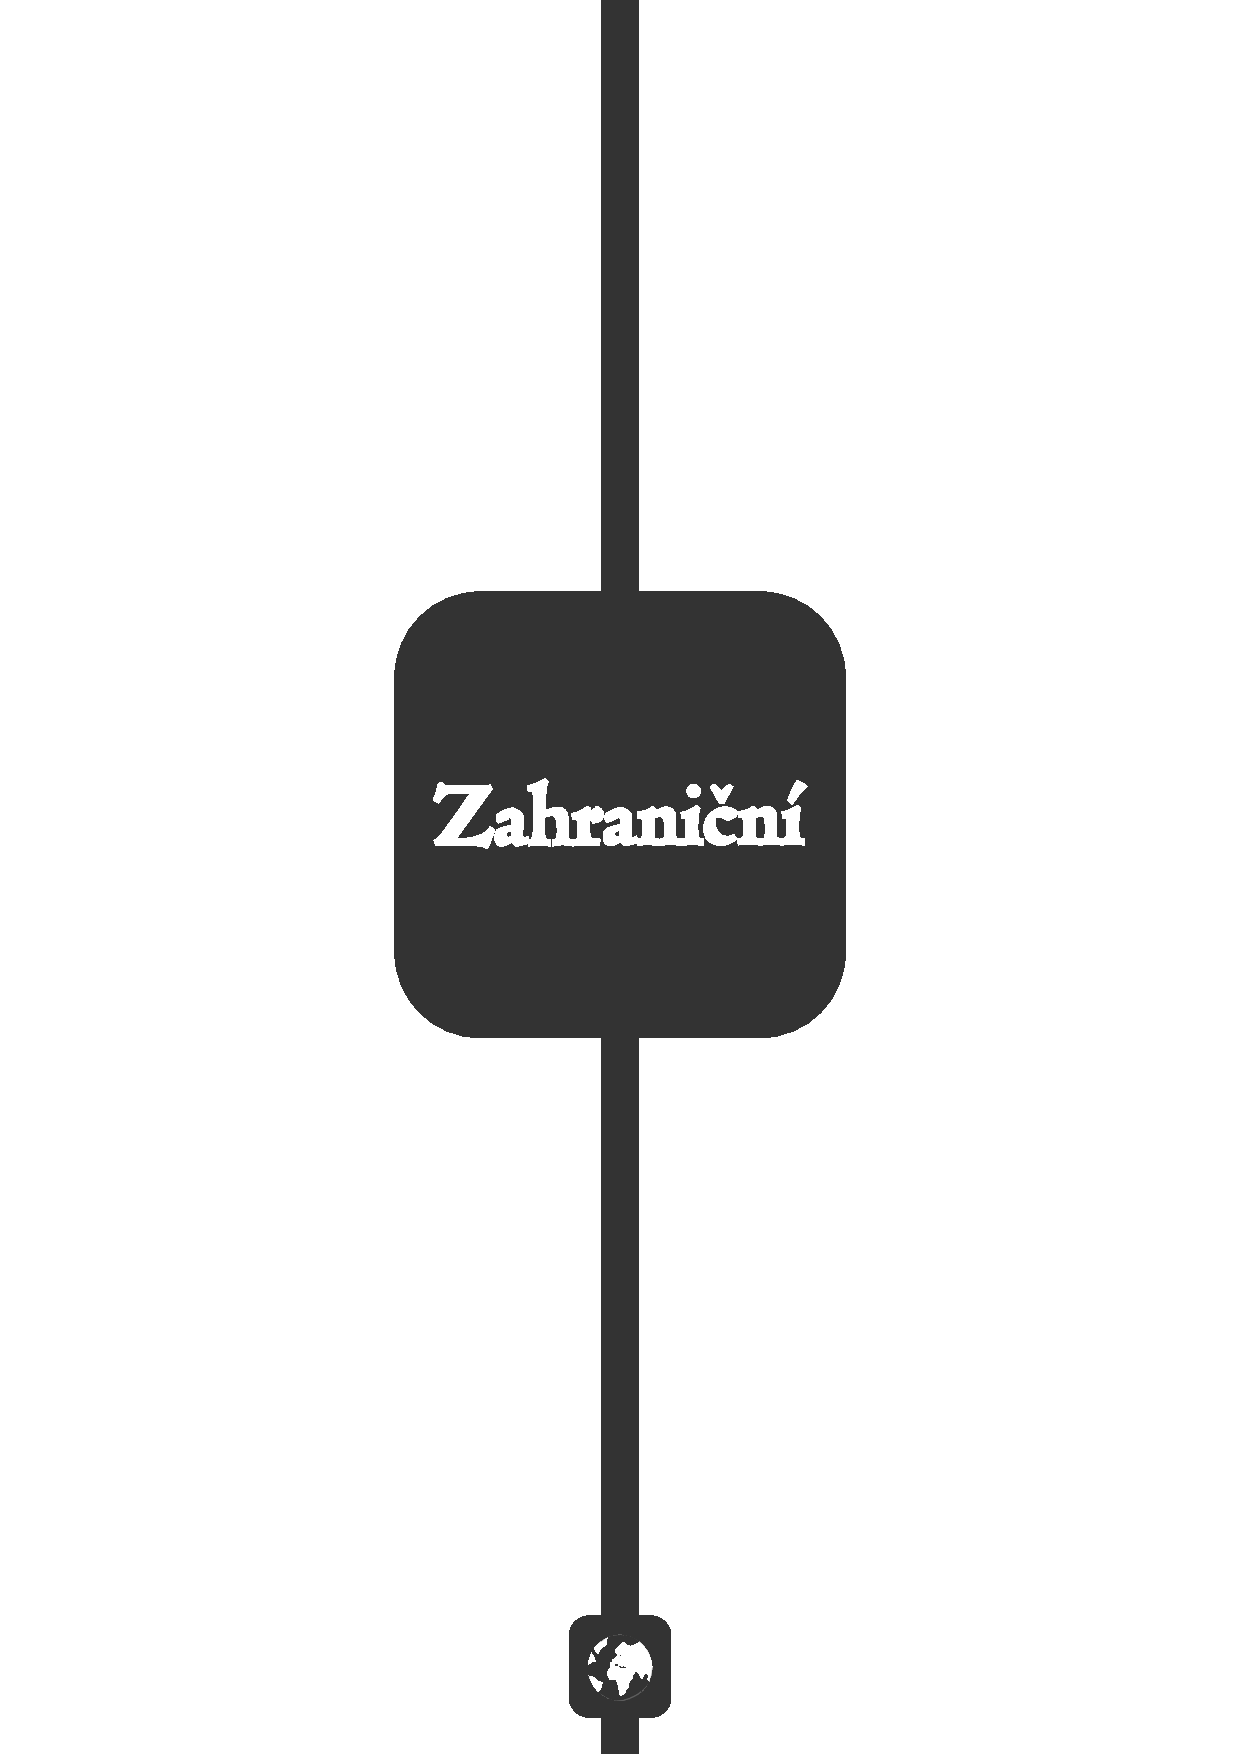
\includepdf[pages=-]{cover/international.pdf}
  % \leavevmode\thispagestyle{empty}\newpage
  \vspace*{\fill}
  \begin{center}
    \Huge\bfseries Zahraniční
  \end{center}
  \vspace*{\fill}
  \pagebreak
  % \sclearpage


  \beginsong{American Pie}[by={\normalsize Don McLean}]
% \transpose{7}
\preferflats
% \caponote[5]
\beginverse
A \[G]long, \[D]long \[E&]time ago,
\[A&]I can still re\[C]member,
how that \[E&]music used to make me \[D]smile.
And \[G]I knew if I \[D]had my \[E&]chance,
that \[A&]I could make those \[C]people dance,
and \[E&]maybe they'd be \[C]happy for a \[D]while.
But \[E&]February \[A&]made me shiver,
with \[E&]every paper \[A&]I'd deliver.
\[C]Bad news \[G]on the \[A&]doorstep;
I \[C]couldn't take \[D]one more step
I \[G]can't re\[D]member \[E&]if I cried,
when I \[A&]read about his \[D]widowed bride;
\[G]something \[D]touched me \[E&]deep inside,
the \[C]day the \[D7]music \[G]died\[C].\[G]
\endverse

\beginchorus
So, \[G]bye-\[C]bye, Miss \[G]American \[D]Pie,
drove my \[G]Chevy to the \[C]levee but the \[G]levee was \[D]dry.
Them \[G]good ole \[C]boys were drinking \[G]whiskey and \[D]rye,
singing \[E&]this'll be the day that I \[A7]die,
\[E&]this'll be the day that I \[D7]die.
\endchorus

\beginverse
\[G]Did you write the \[A&]book of love
and do \[C]you have faith in \[A&]God above,
if the \[E&]Bible \[D]tells you so? 
Now do \[G]you be\[D]lieve in \[E&]rock and roll,
can \[A&]music save your \[C]mortal soul?
And \[E&]can you teach me how to \[A7]dance real \[D7]slow?
\endverse
\beginverse
Well I \[E&]know that you're in \[A&]love with him,
'cause I \[E&]saw you dancing \[A&]in the gym
You \[C]both \[G]kicked off your \[A7]shoes,
man I \[C]dig those rhythm and \[D7]blues!
I was a \[G]lonely \[D]teenage \[E&]bronching buck,
with a \[A&]pink carnation and a \[C]pick-up truck.
But I \[G]knew \[D]I was \[E&]out of luck 
the \[C]day, the \[D7]music \[G]die\[C]d.\[G]
\[G]I started \[D7]singing....
\endverse

\refchorus

\beginverse
Now for \[G]ten years, we've been \[A&]on our own
and \[C]moss grows fat on a \[A&]rolling stone,
but \[E&]that's not how it \[D]used to be.
When the \[G]jester \[D]sang for the \[E&]King and
Queen, in a \[A&]coat he borrowed \[C]from James Dean,
and a \[E&]voice that \[A7]came from you and \[D7]me.
\endverse

\beginverse
Oh, and \[E&]while the king was \[A&]looking down,
the \[E&]jester stole his \[A&]thorny crown;
the \[C]court room \[G]was ad\[A7]journed,
no \[C]verdict was re\[D7]turned.
And while \[G]Lenin \[D]read a \[E&]book on Marx,
the \[A&]quartet practiced \[C]in the park;
\[G]and we sang \[D]dirges \[E&]in the dark,
the \[C]day the \[D7]music \[G]die\[C]d,\[G]
we were \[D7]singing
\endverse

\refchorus

\beginverse
\[G]Helter skelter \[A&]in the summer swelter,
the \[C]birds flew off with a \[A&]fallout shelter;
\[E&]eight miles high and \[D]falling fast.
It \[G]landed \[D]foul \[E&]on the grass,
the \[A&]players tried for a \[C]forward pass
with the \[E&]jester on the \[A7]sidelines in a \[D7]cast.
\endverse
\beginverse
The \[E&]half time air was \[A&]sweet perfume,
while the \[E&]sergeants played a \[A&]marching tune;
we \[C]all got \[G]up to \[A7]dance, but we \[C]never got the \[D7]chance.
'Cause the \[G]players \[D]tried to \[E&]take the field, 
but the \[A&]marching band re\[C]fused to yield
Do \[G]you re\[D]call what \[E&]was revealed,
the \[C]day the \[D7]music \[G]die\[C]d?\[G]
We started \[D7]singing
\endverse

\refchorus

\beginverse
Oh, and \[G]there we were all \[A&]in one place
a \[C]generation \[A&]lost in space
with \[E&]no time left, to start a\[D]gain. 
So come \[G]on, Jack be \[D]nimble, \[E&]jack be quick,
\[A&]Jack flash sat on a \[C]candlestick, 
'cause \[E&]fire is the \[A7]devil's only \[D7]friend.
\endverse
\beginverse
And \[E&]as I watched him \[A&]on the stage,
my \[E&]hands were clenched in \[A&]fists of rage.
No \[C]angel \[G]born in \[A7]hell,
could \[C]break that Satan’s \[D7]spell
And as the \[G]flames climbed \[D]high in\[E&]to the night,
to \[A&]light the sacri\[C]ficial rite
I saw \[G]Satan \[D]laughing \[E&]with delight, 
the \[C]day the \[D7]music \[G]died\[C].\[G]
We were \[D7]singing
\endverse

\refchorus

\beginverse
I \[G]met a \[D]girl who \[E&]sang the blues
and I \[A&]asked her for some \[C]happy news
but \[E&]she just smiled and \[D]turned away.
\[G]I went \[D]down to the \[E&]sacred store,
where I \[A&]heard the music \[C]years before,
but the \[E&]man there said the \[C]music wouldn't \[D]play. 
\endverse

\beginverse
And \[E&]in the streets the \[A&]children screamed,
the l\[E&]overs cried and the \[A&]poets dreamed.
But \[C]not a \[G]word was \[A&]spoken,
the \[C]church bells all were \[D]broken.
And the \[G]three men \[D]I ad\[E&]mire most:
the \[A&]Father, Son and the \[D]Holy Ghost
\[G]They caught the \[D]last train \[E&]for the coast
the \[C]day, the \[D7]music \[G]died.
And they were \[D7]singing
\endverse

\beginchorus
So, \[G]bye-\[C]bye, Miss \[G]American \[D]Pie,
drove my \[G]Chevy to the \[C]levee but the \[G]levee was \[D]dry.
Them \[G]good ole \[C]boys were drinking \[G]whiskey and \[D]rye,
singing \[E&]this'll be the day that I \[A7]die,
\[E&]this'll be the day that I \[D7]die.
\endchorus

\beginchorus
And they were \[D7]singing
\[G]Bye-\[C]bye, Miss \[G]American \[D]Pie, drove my \[G]Chevy to the \[C]levee but the
\[G]levee was \[D]dry. Them \[G]good ole \[C]boys were drinking \[G]whiskey and \[D]rye, singing
\[C]this'll be the \[D7]day that I \[G]die\[C]\[G]
\endchorus
\endsong
  \beginsong{Behind Blue Eyes}[by={\normalsize Limp Bizkit}]
\beginverse
\[E&]No one knows what it's \[G6]like
To be the \[Dsus2]bad man
To be the \[Cadd9]sad man
Be\[A]hind blue eyes
And \[E&]no one knows what it's \[G6]like
To be \[Dsus2]hated
To be \[Cadd9]fated
To telling \[A]only lies
\endverse

\beginchorus
But my \[Cadd9]dreams\[D]
They aren't as \[G]empty
As my \[Cadd9]conscience \[D]seems to \[E]be\[Esus4]\[E]
I have \[H&]hours, only \[Cadd9]lonely
My love is \[D]vengeance
That's never \[Asus2]free
\endchorus

\beginverse
\[E&]No one knows what it's \[G6]like
To feel these \[Dsus2]feelings
Like I \[Cadd9]do
And I blame \[Asus2]you
No \[E&]one bites back as \[G6]hard
On their \[Dsus2]anger
None of my \[Cadd9]pain an' woe
Can show \[Asus2]through
\endverse

\refchorus

\beginverse
\[E&] \[G6] \[Dsus2]\[Dsus2]\[Cadd9]\[Cadd9] \[Asus2] \[Asus2]\vspace{-0.5cm}
 \textit{Discover \ldots L.I.M.P. \ldots Say it \ldots }
\endverse

\beginverse
\[E&]No one knows what it's \[G6]like
To be mis\[Dsus2]treated
To be de\[Cadd9]feated
Be\[Asus2]hind blue eyes
And \[E&]no one knows how to \[G6]say
That they're \[Dsus2]sorry
And don't \[Cadd9]worry
I'm not \[Asus2]telling lies
\endverse

\refchorus

\beginverse
No \[E&]one knows what it's \[G6]like
To be the \[Dsus2]bad man
To be the \[Cadd9]sad man
Be\[A]hind blue eyes
\endverse
\endsong
  \beginsong{Bella Ciao}[by={\normalsize Traditional}]
\beginverse
\[A&]Una mattina mi son svegliato,
O bella, ciao! Bella, ciao!
Bella, c\[Am7]iao, ciao, ciao!
Una mat\[D&]tina mi son svegl\[A&]iato
e ho tro\[E7]vato l'invas\[A&]or.
\endverse

\beginverse
\[A&]O partigiano, portami via,
O bella, ciao! Bella, ciao!
Bella, c\[Am7]iao, ciao, ciao!
O partigi\[D&]ano, portami \[A&]via,
ché mi s\[E7]ento di mor\[A&]ir.
\endverse

\beginverse
\[A&]E se io muoio da partigiano,
O bella, ciao! Bella, ciao!
Bella, c\[Am7]iao, ciao, ciao!
E se io m\[D&]uoio da partig\[A&]iano,
tu mi \[E7]devi seppell\[A&]ir.
\endverse

\beginverse
\[A&]Seppellire lassù in montagna,
O bella, ciao! Bella, ciao!
Bella, c\[Am7]iao, ciao, ciao!
E seppel\[D&]lire lassù in mon\[A&]tagna
Sotto l'\[E7]ombra di un bel fi\[A&]or.
\endverse

\beginverse
\[A&]E le genti che passeranno
O bella, ciao! Bella, ciao!
Bella, c\[Am7]iao, ciao, ciao!
E le g\[D&]enti che passe\[A&]ranno
Ti dir\[E7]anno ``Che bel fi\[A&]or!''
\endverse

\beginverse
\[A&]``È questo il fiore del partigiano'',
O bella, ciao! Bella, ciao!
Bella, c\[Am7]iao, ciao, ciao!
``È questo il \[D&]fiore del partig\[A&]iano
morto \[E7]per la liber\[A&]tà!'' \rep{2}
\endverse
\endsong

  \beginsong{Boxer}[by={\normalsize Simon \& Garfunkel}]
\caponote[2]
\beginverse
\[A]I am just a poor boy, though my story's seldom \[F#&]told
I have \[E]squandered my resistance
For a \[D]pocketful of mumbles such are \[A]promises
All lies and \[F#&]jest still a \[E]man hears what he \[D]wants to hear
And disregards the \[A]rest\[E]\[D]\[E]\[A]
\endverse

\beginverse
When I \[A]left my home and family I was no more than a \[F#&]boy
In the \[E]company of strangers
In the \[D]quiet of a railway station \[A]running scared
Laying \[F#&]low seeking \[E]out the poorer \[D]quarters where the ragged people \[A]go
Looking \[E]for the places \[D]only \[E]they would \[A]know
\endverse

\beginchorus
   Lie-la-\[F#&]lie
Lie-la-\[C#&]la-la-la lie-la-lie
Lie la \[F#&]lie
Lie-la \[E]la la la la lie la la la la \[A]lie \[(F#&)]
\endchorus

\beginverse
Asking \[A]only workmans wages I come looking for a \[F#&]job
But I get no \[E]offers
Just a \[D]come-on from the whores on Seventh \[A]Avenue
I do de\[F#&]clare there were \[E]times when I was \[D]so lonesome I took some comfort \[A]there
La-la-\[E]la-la-la-la-la\[A]
\endverse

\refchorus

\beginverse
Then I'm \[A]laying out my winter clothes
And wishing I was \[F#&]gone
Going \[E]home where the \[E7]New York City winters aren't \[A]bleeding me
\[C#&] Leading me-\[F#&]e, going \[E]home\[A]
\endverse

\beginverse
In the \[A]clearing stands a boxer and a fighter by his \[F#&]trade
And he \[E]carries the reminders
Of ev'ry glove that laid him down or \[A]cut him 'till he cried out
In his anger and his \[F#&]shame
"I am \[E]leaving, I am \[D]leaving."  But the fighter still re\[A]mains
Hm, hm, \[E]hm\[D]\[E]\[A]
\endverse

\refchorus \rep{8}
\endsong
  \beginsong{Bring Me To Life}[by={\normalsize Evanescence}]
\caponote[1]
\beginverse
\[E&]How can you see into my e\[A&]yes like open doors?
\[E&]Leading you down into my \[A&]core where I've become so numb
\[E&]Without a soul, \[A&]my spirit's sleeping somewhere \[E&]cold
Until you find it there and \[A&]lead it back home
\endverse

\beginchorus
\[E&]\textit{(Wake me up)} Wake me up in\[G]side
\textit{(I can't wake up)} Wake me up in\[D]side
\textit{(Save me)} Call my name and save me from the \[E&]dark
\textit{(Wake me up)} Bid my blood to \[G]run
\textit{(I can't wake up)} Before I come \[D]undone
\textit{(Save me)} Save me from the nothing I've be\[E&]come \[(C)]
\endchorus

\beginverse
\[E&]Now that I know what I'm \[C]without
You can't just leave me
Brea\[E&]the into me and make me \[C]real
Bring me to life
\endverse

\refchorus

\beginverse
\[C] Bring \[D]me to l\[E&]ife \textit{(I've been living a lie, there's nothing inside)}
\[C] Bring \[D]me to \[E&]life \[E&]\[D/F#]\[G]\[H&]
\endverse

\beginverse
\[A&]Frozen in\[Em/G]side without your \[D/F#]touch
Without your \[E&]love,  \[D/F#]darling
\[A&]Only \[G]you are the \[H]life among the dead
\endverse

\beginverse
\[E&]All this time I can't believe I couldn't see
\[E&]Kept in the dark but you were there in front of me
\[C/E]I've been sleeping a thousand years it seems
\[C/E]Got to open my eyes to everything
\[E&]Without a thought, without a voice, without a soul
\[E&]Don't let me die here
There must be some\[C]thing more
Bring \[D]me to l\[E&]ife
\endverse

\refchorus

\beginverse
\[C] Bring \[D]me to l\[E&]ife  \textit{(I've been living a lie, there's nothing inside)}
\[C]Bring \[D]me to \[E&]life
\endverse

\beginverse
\[E&]\[D]\[A&]\[G]\[D/F#]
\endverse
\endsong
  \beginsong{Californication}[by={\normalsize Red Hot Chilli Peppers}]
\beginverse
\[A&]\[F]\[A&]\[F]
\vspace{-0.5cm}
\endverse

\beginverse
\[A&]Psychic spies from China
Try to \[F]steal your mind's elation
\[A&]Little girls from Sweden
Dream of \[F]silver screen quotations
And \[C]if you want these \[G]kind of dreams
It's \[F]Californi\[D&]cation \[A&]\[F]\[A&]\[F]
\endverse

% \beginverse
% \[A&]\[F]\[A&]\[F]
% \vspace{-0.5cm}
% \endverse

\beginverse
It's the\[A&] edge of the world
And all of \[F]western civilization
The \[A&]sun may rise in the East
At least it \[F]settled in a fine location
It's \[C]understood that \[G]Hollywood
sells \[F]Californi\[D&]cation \[A&]\[F]\[A&]\[F]
\endverse

% \beginverse
% \[A&]\[F]\[A&]\[F]
% \vspace{-0.5cm}
% \endverse

\beginverse
\[A&]Pay your surgeon very well
To \[Fmaj7]break the spell of aging
Ce\[A&]lebrity skin, is this your chin?
Or \[Fmaj7]is that war you're waging?
\[A&]   First born unic\[Fmaj7]orn
\[A&]   Hardcore soft p\[Fmaj7]orn
\endverse

\beginchorus
\[C]Dream of Cali\[G]fornic\[D&]ation\[A&]
\[C]Dream of Cali\[G]forni\[D&]cation
\[C]Dream of Cali\[G]fornic\[D&]ation\[A&]
\[C]Dream of Cali\[G]forni\[D&]cation \[A&]\[F]\[A&]\[F]
\endchorus

% \beginverse
% \[A&]\[F]\[A&]\[F]
% \vspace{-0.5cm}
% \endverse

\beginverse
\[A&]Marry me girl, be my fairy to the world
Be my \[F]very own constellation
A \[A&]teenage bride with a baby inside
Getting \[F]high on information
And \[C]buy me a star on the \[G]boulevard
\endverse


\beginverse
It's \[F]Californi\[D&]cation \[A&]\[F]\[A&]\[F]
\endverse

% \beginverse
% \[A&]\[F]\[A&]\[F]
% \vspace{-0.5cm}
% \endverse

\beginverse
\[A&]Space may be the final frontier
But it's \[F]made in a Hollywood basement
And \[A&]Cobain can you hear the spheres
Singing \[F]songs off station to station?
And \[C]Alderaan's not \[G]far away
It's \[F]Californi\[D&]cation
\endverse

\beginverse
\[A&]Ooooo - \[Fmaj7]ooooh   \[A&]Oooo -  \[Fmaj7]ooooh
\endverse

\beginverse
\[A&]Born and raised by those who praise
Con\[Fmaj7]trol of population
\[A&]Everybody's been there and
I d\[Fmaj7]on't mean on vacation
\[A&]   First born unic\[Fmaj7]orn
\[A&]   Hardcore soft p\[Fmaj7]orn
\endverse

\refchorus

% \beginverse
% \[A&]\[F]\[A&]\[F]
% \vspace{-0.5cm}
% \endverse

\beginverse
Des\[A&]truction leads to a very rough road
But it \[F]also breeds creation
And \[A&]earthquakes are to a girl's guitar
They're \[F]just another good vibration
And \[C]tidal waves couldn't \[G]save the world
From \[F]Californi\[D&]cation
\endverse

\beginverse
\[A&]Ooooo - \[Fmaj7]ooooh   \[A&]Oooo -  \[Fmaj7]ooooh
\endverse

\beginverse
\[A&]Pay your surgeon very well
To \[Fmaj7]break the spell of aging
\[A&]Sicker than the rest, there is no test
But \[Fmaj7]this is what you're craving
\[A&]   First born unic\[Fmaj7]orn
\[A&]   Hardcore soft p\[Fmaj7]orn
\endverse

\refchorus
% \beginchorus
% \[C]Dream of Cali\[G]fornic\[D&]ation\[A&]
% \[C]Dream of Cali\[G]forni\[D&]cation
% \[C]Dream of Cali\[G]fornic\[D&]ation\[A&]
% \[C]Dream of Cali\[G]forni\[D&]cation 
% \endchorus

\endsong
  \beginsong{Can't Stop}[by={\normalsize Red Hot Chilli Peppers}]
\beginverse
\[E&]Can't stop addicted to the shindig
\[D]Chop top he says I'm gonna win big
\[H&]Choose not a life of imitation
\[C]Distant cousin to the reservation
\endverse
\beginverse
\[E&]Defunct the pistol that you pay for
\[D]This punk the feeling that you stay for
\[H&]In time I want to be your best friend
\[C]Eastside love is living on the westend
\endverse
\beginverse
\[E&]Knocked out but boy you better come to
\[D]Don't die you know the truth as some do
\[H&]Go write your message on the pavement
\[C]Burn so bright I wonder what the wave meant
\endverse
\beginverse
\[E&]White heat is screaming in the jungle
\[D]Complete the motion if you stumble
\[H&]Go ask the dust for any answers
\[C]Come back strong with fifty belly dancers
\endverse

\beginchorus
The w\[G]orld I love
The t\[D]ears I've dropped
To \[H&]be part of
the w\[C]ave can't stop
\[G]Ever wonder \[D]if it's a\[H&]ll for y\[C]ou
The w\[G]orld I love
The tr\[D]ains I hop
To \[H&]be part of
The w\[C]ave can't stop
C\[G]ome and tell me wh\[D]en it's ti\[H&]me \[C]to
\endchorus

\beginverse
\[E&]Sweetheart is bleeding in the snowcone
\[D]So smart she's leading me to ozone
\[H&]Music the great communicator
\[C]Use two sticks to make it in the nature
\endverse
\beginverse
\[E&]I'll get you into penetration
\[D]The gender of a generation
\[H&]The birth of every other nation
\[C]Worth your weight the gold of meditation
\endverse
\beginverse
\[E&]This chapter's going to be a close one
\[D]Smoke rings I know you're going to blow one
\[H&]All on a spaceship persevering
\[C]Use my hands for everything but steering
\endverse
\beginverse
\[E&]Can't stop the spirits when they need you
\[D]Mop tops are happy when they feed you
\[H&]Jay butterfly is in the treetop
\[C]Birds that blow the meaning into bebop
\endverse

\refchorus

\beginverse
\[E&]Wait a minute I'm p\[D]assing out, win or l\[H&]ose, just like y\[C]ou
\[E&]Far more shockin' than an\[D]ything I ever k\[H&]new, how 'bout \[C]you
\[E&]Ten more reasons w\[D]hy I need somebody \[H&]new, just like \[C]you
\[E&]Far more shockin' than an\[D]ything I ever k\[H&]new, right on c\[C]ue
\endverse

\beginverse
\[E&]Can't stop addicted to the shindig
\[D]Chop top he says I'm gonna win big
\[H&]Choose not a life of imitation
\[C]Distant cousin to the reservation
\endverse
\beginverse
\[E&]Defunct the pistol that you pay for
\[D]This punk the feeling that you stay for
\[H&]In time I want to be your best friend
\[C]Eastside love is living on the westend
\endverse
\beginverse
\[E&]Knocked out but boy you better come to
D\[D]on't die you know the truth as some do
\[H&]Go write your message on the pavement
\[C]Burn so bright I wonder what the wave meant
\endverse
\beginverse
\[E&]Kick start the golden generator
\[D]Sweet talk but don't intimidate her
\[H&]Can't stop the Gods from engineering
\[C]Feel no need for any interfering
\endverse
\beginverse
\[E&]Your image in the dictionary
\[D]This life is more than ordinary
\[H&]Can I get two maybe even three of these
\[C]Comin' from space to teach you of the Pliedes
\endverse
\beginverse
Can't stop the spirits when they need you
This life is more than just a read-thru
\endverse
\endsong
  \beginsong{Castle Of Glass}[by={\normalsize Linkin Park}]
\transpose{-4}
\caponote[4]
\beginverse
\[C#&]\[C#&]\[H]\[F#&] \rep{3} \[A]\[H]\[C#&] \vspace*{-0.5cm}
\endverse

\beginverse
\[C#&]Take me down to the river bend
\[C#&]Take me down to the fighting end
\[H]Wash the poison from off my skin
\[C#&]Show me how to be whole again
\[C#&]Fly me up on a silver wing
\[C#&]Past the black where the siren sing
\[H]Warm me up in a nova's glow
\[C#&]And drop me down to the dream below
\endverse

\beginchorus
Cause I'm \[A]only a cr\[E]ack in this \[H]castle of\[C#&] glass
Hardly a\[A]nything t\[E]here for you to \[H]see
For you to s\[C#&]ee
\endchorus

\beginverse
\[C#&]\[C#&]\[H]\[F#&] \rep{2} \vspace*{-0.5cm}
\endverse

\beginverse
\[C#&]Bring me home in the blinding dream
\[C#&]Through the secrets that I have seen
\[H]Wash the sorrow from off my skin
\[C#&]And show me how to be whole again
\endverse

\refchorus

\beginverse
\[C#&]\[C#&]\[H]\[F#&]\[C#&]\[C#&]\[C#&]\[C#&] \rep{2} \vspace*{-0.5cm}
\endverse

\beginverse
Cause I'm \[A]only a cr\[E]ack in this \[H]castle of\[C#&] glass
I'll be a\[A]nything \[E]else I need to \[H]be
\endverse

\beginchorus
Cause I'm \[A]only a cr\[E]ack in this \[H]castle of\[C#&] glass
Hardly a\[A]nything th\[E]ere for you to \[H]see
For you to s\[C#&]ee\[C#&]\[H]\[F#&]
For you to s\[C#&]ee\[C#&]\[H]\[F#&]\[C#&]
\endchorus
\endsong
  \beginsong{Comfortably Numb}[by={\normalsize Pink Floyd}]
\beginverse
\[Hsus2]       \[H&]Hello?
Is there anybody \[A]in there?
Just nod if you can \[G]hear me\[G/F#]\[E&]
Is there \[H&]anyone at home?
\[Hsus2]Come on now\[H&]
I hear you're \[A]feeling down
\[G]I can ease \[G/F#]your pai\[E&]n
And get you \[H&]on your feet again
\endverse

\beginverse
\[Hsus2] \[H&]Relax
I'll need some infor\[A]mation first
\[G]Just the basic\[G/F#] fact\[E&]s
Can you \[H&]show me where it hurts?
\endverse

\beginchorus
\[D]There is no pain you are re\[A]ceding
\[D]A distant ship smoke on the ho\[A]rizon
\[G]   Y\[C]ou are only coming through in \[G]waves
 Y\[C]our lips move but I can't hear what you'\[G]re saying
When \[D]I was a child I had a \[A]fever
My \[D]hands felt just like two bal\[A]loons
\[G]  No\[C]w I've got that feeling once a\[G]gain, I can't explain,
You would not \[C]understand, this is not how I \[G]am
\endchorus

\beginverse
\[A]I   \[G]     \[Cadd9]       have be\[G]come comfortably \[D]numb. \vspace{-0.5cm}
\endverse
\beginverse
\[D]\[A]\rep{2}\[C]\[G]\rep{2} \vspace{0.5cm}
\[A]I   \[G]    \[Cadd9]  have be\[G]come comfortably \[D]numb.
\endverse

\beginverse
\[H&]O.K.
Just a little \[A]pinprick
There'll be no more \[G]aaaaa\[E&]aaah!
But you may \[H&]feel a little sick
\[Hsus2]Can you stand \[H&]up?
I do believe it's \[A]working, good
That'll keep you \[G]going through the s\[E&]how
Come \[H&]on it's time to go.
\endverse

\beginchorus
\[D]There is no pain, you are re\[A]ceding
\[D]A distant ship smoke on the ho\[A]rizon
\[G]    \[C]You are only coming through in \[G]waves
   Y\[C]our lips move but I can't hear what you\[G]'re saying
When \[D]I was a child, I caught a \[A]fleeting glimpse
\[D]Out of the corner of my \[A]eye
\[G]    \[C]I turned to look but it was \[G]gone
I cannot put my finger \[C]on it now
The child is grown, the \[G]dream is gone
\endchorus

\beginverse
And  \[A]I     \[G]     \[Cadd9] have bec\[G]ome comfortably n\[D]umb.
\endverse

\beginverse
\[H&]\[A]\[G]\[E&]\[H&]
\endverse
\endsong
  \beginsong{Creep}[by={\normalsize Radiohead}]
\beginverse
\[G]\[H]\[C]\[C&] \chordskip
\endverse
\beginverse
When you were here be\[G]fore, couldn't look you in the \[H]eyes
You're just like an \[C]angel, your skin makes me \[C&]cry
You float like a \[G]feather in a beautiful \[H]world
I wish I was \[C]special, you're so fucking \[C&]special
\endverse

\beginchorus
But I'm a \[G]creep, I'm a \[H]weirdo
What the hell am I doing \[C]here? I don't be\[C&]long here
\endchorus

\beginverse
I don't care if it \[G]hurts, I wanna have con\[H]trol
I want a perfect \[C]body, I want a perfect \[C&]soul
I want you to \[G]notice when I'm not a\[H]round
You're so fucking \[C]special, I wish I was \[C&]special
\endverse

\refchorus

\beginverse
Oooh, oooh, \[G]she's running out the \[H]door\ldots
\[C]She's running out, she \[C&]run, run, run\ldots
\[G]Ruu\[H]un\ldots
\[C]Ruu\[C&]{un\ldots}
\endverse

\beginverse
Whatever makes you \[G]happy, whatever you \[H]want
You're so fucking \[C]special, I wish I was \[C&]special
\endverse

\refchorus
\endsong
  \beginsong{Drunken Sailor}[by={\normalsize Traditional}]
\beginverse
\[E&]What shall we do with the drunken sailor?
\[D]What shall we do with the drunken sailor?
\[E&]What shall we do with the drunken sailor?
\[E&]Ear\[D]ly in the \[E&]morning
\endverse

\beginchorus
\[E&]Way hay and up she rises
\[D]Way hay and up she rises
\[E&]Way hay and up she rises
\[E&]Ear\[D]ly in the m\[E&]orning
\endchorus


\beginverse
Put him in the long boat 'til he's sober\ldots
\endverse
\vspace{-0.5cm}
\beginverse
Pull out the plug and wet him all over\ldots
\endverse
\vspace{-0.5cm}
\beginverse
Put him in the scuppers with the hosepipe on him\ldots
\endverse
\vspace{-0.5cm}
\beginverse
Shave his belly with a rusty razor\ldots
\endverse
\vspace{-0.5cm}
\beginverse
Put him in bed with the captain's daughter\ldots
\endverse
\vspace{-0.5cm}
\beginverse
That's what we do with the drunken sailor\ldots
\endverse

\endsong
  \beginsong{Demons}[by={\normalsize Imagine Dragons}]
\caponote[3]
\beginverse
When the da\[C]ys are cold
And the car\[G]ds all fold
And the sai\[A&]nts we see
Are all ma\[F]de of gold
When your d\[C]reams all fail
And the one\[G]s we hail
Are the wor\[A&]st of all
And the bl\[F]ood's run stale
\endverse

\beginverse
\[C]  I wanna hide the \[G]truth
I wanna shelter \[A&]you
But with the beast \[F]inside
There's nowhere we can \[C]hide
No matter what we \[G]breed
We still are made of \[A&]greed
This is my kingdom \[F]come
This is my kingdom \[C]come
\endverse

\beginchorus
\[C]  When you feel my \[G]heat
Look into my \[A&]eyes
It's where my demons \[F]hide
It's where my demons \[C]hide
Don't get too \[G]close
It's dark in\[A&]side
It's where my demons \[F]hide
It's where my demons \[C]hide
\endchorus

\beginverse
When the cu\[C]rtain's call
Is the last\[G] of all
When the li\[A&]ghts fade out
All the si\[F]nners crawl
So they du\[C]g your grave
And the mas\[G]querade
Will come c\[A&]alling out
At the mes\[F]s you made
\endverse

\beginverse
\[C]  Don't wanna let you \[G]down
But I am hell \[A&]bound
Though this is all for \[F]you
Don't wanna hide the \[C]truth
No matter what we \[G]breed
We still are made of \[A&]greed
This is my kingdom \[F]come
This is my kingdom \[C]come
\endverse

\refchorus

\beginverse
\[C]  They say it's what you \[G]make
I say it's up to \[A&]fate
It's woven in my \[F]soul
I need to let you \[C]go
Your eyes, they shine so \[G]bright
I wanna save that \[A&]light
I can't escape this now
Unless you show me \[C]how
\endverse

\refchorus
\endsong
  \beginsong{Forever Young}[by={\normalsize Alphaville}]
\beginverse
\[C]  Let's dance in \[G]style, let's dance for \[A&]a while
Heaven can \[F]wait we're only watching the \[G]skies
Hoping for the \[D&]best, but expecting the \[F]worst
Are you gonna drop the \[Fmaj7]bomb or not?\[G6]\[C]
\endverse

\beginverse
\[C]Let us stay young\[G] or let us live forever\[A&]
We don't ha\[F]ve the power, but we never sa\[G]y never
Sitting in the \[D&]sandpit, life is a short\[F] trip
The music's for the \[Fmaj7]sad man\[G6]\[C]
\endverse

\beginverse
\[C]Can you imagine w\[G]hen this race is won\[A&]
Turn our go\[F]lden faces into the sun\[G]
Praising our le\[D&]aders, we're getting in \[F]tune
The music's played \[Fmaj7]by the \[G6]mad man\[C]
\endverse

\beginchorus
\[C]  Forever \[G]young
I want to \[A&]be forever \[F]young
\[G] Do you really want to \[A&]live forever?
\[F] Forever\[G], and ever
\[C]  Forever \[G]young,
I want to \[A&]be forever \[F]young
\[G]Do you really want to \[A&]live forever?
\[F]   \[G]  Forever \[C]young.
\endchorus

\beginverse
\[C]Some are like wat\[G]er, some are like the h\[A&]eat
Some are th\[F]e melody and some are the \[G]beat
Sooner or later\[D&] they all will be gone\[F]
Why don't they stay \[Fmaj7]young?\[G6]\[C]
\endverse

\beginverse
\[C]It's so hard to g\[G]et old without a cause\[A&]
I don't wan\[F]t to perish like a fading hor\[G]se
Youth's like diam\[D&]onds in the sun\[F]
And diamonds are fo\[Fmaj7]rever\[G6]\[C]
\endverse

\beginverse
\[C]So many adventure\[G]s could've happen today\[A&]
So many son\[F]gs we forgot to play\[G]
So many dreams \[D&]swinging out of the blue\[F]
Oh let it come \[Fmaj7]true\[G6]\[C]
\endverse

\refchorus \rep{2}
\endsong
  \beginsong{Hallelujah}[by={\normalsize Leonard Cohen}]
\beginverse
Now I've \[C]heard there was a se\[A&]cret chord
That \[C]David played, and it pl\[A&]eased the Lord
But \[F]you don't really \[G]care for music, do y\[C]ou?\[G]
It \[C]goes like this the \[F]fourth, the \[G]fifth
The \[A&]minor fall, the \[F]major lift
The \[G]baffled king com\[E7]posing Halle\[A&]lujah
Halle\[F]lujah, Halle\[A&]lujah, Halle\[F]lujah, Halle\[C]lu-\[G]u-\[C]jah\[G]
\endverse

\beginverse
Your \[C]faith was strong, but you \[A&]needed proof
You \[C]saw her bathing \[A&]on the roof
Her \[F]beauty and the \[G]moonlight over\[C]threw ya\[G]
She \[C]tied you to a \[F]kitchen \[G]chair
She \[A&]broke your throne, and she \[F]cut your hair
And \[G]from your lips she \[E7]drew the Halle\[A&]lujah
Halle\[F]lujah, Halle\[A&]lujah, Halle\[F]lujah, Halle\[C]lu-\[G]u-\[C]jah\[G]
\endverse

\beginverse
You \[C]say I took the \[A&]name in vain
\[C]I don't even \[A&]know the name
But \[F]if I did, well \[G]really, what's it \[C]to ya?\[G]
There's a \[C]blaze of light in \[F]every \[G]word
It \[A&]doesn't matter \[F]which you heard
The \[G]holy or the \[E7]broken Halle\[A&]lujah
Halle\[F]lujah, Halle\[A&]lujah, Halle\[F]lujah, Halle\[C]lu-\[G]u-\[C]jah\[G]
\endverse

\beginverse
I \[C]did my best, it \[A&]wasn't much
I \[C]couldn't feel, so I \[A&]tried to touch
I've \[F]told the truth, I \[G]didn't come to fool y\[C]a\[G]
And \[C]even though it \[F]all went \[G]wrong
I'll \[A&]stand before the \[F]Lord of Song
With \[G]nothing on my \[E7]tongue but Halle\[A&]lujah
\endverse

\beginverse
Halle\[F]lujah, Halle\[A&]lujah, Halle\[F]lujah, Halle\[C]lu\[G]jah \rep{2}\[C]
\endverse
\endsong
  % Hsus4 = x24400
% Eadd9 = 024100
% Emadd9 = 024000

\beginsong{Happy Christmas (War Is Over)}[by={\normalsize John Lennon}]
\beginverse
So this is \[A]Christmas\[Asus2]\[Asus4]
And \[A]what have you \[H&]done\[Hsus2]\[Hsus4]
\[H&]Another year \[Esus4]over\[E]\[Eadd9]
And a \[E]new one just be\[A]gun\[Asus2]\[Asus4]
\endverse
\beginverse
And \[A]so this is \[D]Christmas\[Dsus2]\[Dsus4]
I \[D]hope you have \[E&]fun\[Emadd9]\[Esus4]
The \[E&]near and the dear \[Asus4]ones\[A]\[Asus2]
The \[A]old and the \[D]young\[Dsus2]\[Dsus4]
\endverse

\beginchorus
A \[D]very Merr\[G]y Christmas
And a happy New \[A]Year
Let's hope it's a \[E&]good one\[G]
Without any \[D]fear\[E7]
\endchorus

\beginverse
And so this is \[A]Christ\[Asus2]mas\[Asus4]
For \[A]weak and for s\[H&]trong\[Hsus2]\[Hsus4]
The \[H&]rich and the \[Esus4]poor ones\[E]\[Eadd9]
The \[E]road is so l\[A]ong\[Asus2]\[Asus4]
\endverse
\beginverse
And \[A]so Happy \[D]Christmas\[Dsus2]\[Dsus4]
For \[D]black and for \[E&]white\[Emadd9]\[Esus4]
For \[E&]yellow and \[Asus4]red ones\[A]\[Asus2]
Let's \[A]stop all the \[D]fight\[Dsus2]\[Dsus4]\[D]
\endverse

\refchorus

\beginverse
And so this is \[A]Christmas\[Asus2]\[Asus4]
And \[A]what have we \[H&]done\[Hsus2]\[Hsus4]
\[H&]Another year \[Esus4]over\[E]\[Eadd9]
A \[E]new one just \[A]begun\[Asus2]\[Asus4]
\endverse
\beginverse
And \[A]so Happy \[D]Christmas\[Dsus2]\[Dsus4]
We \[D]hope you have \[E&]fun\[Emadd9]\[Esus4]
The \[E&]near and the dear \[Asus4]ones\[A]\[Asus2]
The \[A]old and the \[D]young\[Dsus2]\[Dsus4]
\endverse

\refchorus

\beginverse
 \[A]War   \[Asus2]is        \[Asus4]o     -   \[A]ver
 \[H&]If     \[Hsus2]you       \[Hsus4]want      \[H&]it
 \[Esus4]War       \[E]is    \[Eadd9]o     -   \[E]ver
 \[A]Now\[Asus2]\[Asus4]\[A]
\endverse
\endsong
  \beginsong{Help!}[by={\normalsize The Beatles}]
\beginverse
\[H&]Help! I need somebody
\[G]Help! Not just any\[G/F#]body
\[E]Help! You know I need someone,
\[A]Help!
\endverse

\beginverse
\[A]When I was younger, so much y\[C#&]ounger than today,
\[F#&]I never needed anybody's h\[D]elp in a\[G]ny w\[A]ay.
But now those days are gone I'm \[C#&]{not so} self-assured,
\[F#&]Now I find I've changed my mind, I've op\[D]ened \[G]up the d\[A]oors.
\endverse

\beginchorus
H\[H&]elp me if you can I'm feeling down, and I d\[G]o appreciate you being 'round\[G/F#].
H\[E]elp me get my feet back on the ground, won't you pl\[A]ease please help me.
\endchorus

\beginverse
And now my life has changed in \[C#&]{oh so} many ways,
\[F#&]My independence seemed to v\[D]anish \[G]in the h\[A]aze.
But every now and then I \[C#&]feel so insecure,
\[F#&]I know that I just need you like I've ne\[D]ver d\[G]one be\[A]fore.
\endverse

\refchorus

\beginverse
\[A]When I was younger (\ldots)
\endverse

\refchorus

\beginverse
Help me, help\[A] me, \[A6]ooo.
\endverse
\endsong
  \beginsong{Here Comes The Sun}[by={\normalsize The Beatles}]
\beginchorus
\[A]  Here \[Asus2]comes \[A]the sun
\[D]   Here comes the \[H7]sun and I say
\[A]  It's all right.
\endchorus

\beginverse
\[A]  Little d\[Asus2]arling,\[A] it's been a
 \[D] Long cold lonely \[E7]winter.
 \[A] Little d\[Asus2]arling,\[A] it feels like
  \[D]Years since it's been \[E7]here.
\endverse

\refchorus

\beginverse
  \[A] Little d\[Asus2]arling,\[A] the smiles
   Ret\[D]urning to their \[E7]faces.
  \[A] Little d\[Asus2]arling,\[A] it feels like
   \[D]Years since it's been\[E7] clear.
\endverse

\refchorus

\beginverse
\[C]Sun  \[G]Sun  \[D/F#]Sun   \[D]here it \[A]comes.\[E7] \rep{5}
\endverse

\beginverse
\[E7]\[E7sus4]\[E7]\[E7sus4] \vspace*{-0.5cm}
\endverse

\beginverse
\[A] Little d\[Asus2]arling,\[A] I feel that
 \[D]Ice is slowly \[E7]melting.
\[A] Little d\[Asus2]arling,\[A] it feels like
 \[D]Years since it's been \[E7]clear.
\endverse

\refchorus
\endsong
  \beginsong{Hey Jude}[by={\normalsize The Beatles}]
\caponote[3]
\beginverse
Hey J\[D]ude don't make it b\[A]ad
Take a s\[A7]ad song \[A7sus4]{and make} it b\[D]etter
Rem\[G]ember to let her into your h\[D]eart
Then you can st\[A]art to m\[A7]ake it bett\[D]er.
\endverse

\beginverse
Hey J\[D]ude don't be afr\[A]aid
You were m\[A7]ade to \[A7sus4]{go out and} g\[D]et her
The m\[G]inute you let her under your sk\[D]in
Then you beg\[A]in to m\[A7]ake it bett\[D]er.
\endverse

\beginverse
\[D]\[Dmaj7]\[D7]
\vspace{-0.5cm}
\endverse

\beginchorus
And any time you feel the p\[G]ain, Hey J\[Hm7]ude, refr\[E&]ain.
Don't carry the w\[A7]orld upon your sh\[D]oulders.\[D]\[Dmaj7]\[D7]
For well you know that it's a f\[G]ool who pl\[Hm7]ays it c\[E&]ool
By making his w\[A7]orld a little c\[D]older
\endchorus

\beginverse
\[D]Na na na \[D7]na na \[A7]na na na na
\endverse

\beginverse
Hey J\[D]ude don't let me d\[A]own
You have f\[A7]ound her \[A7sus4]{now go and} g\[D]et her.
Rem\[G]ember to let her into your h\[D]eart
Then you can st\[A]art to m\[A7]ake it bett\[D]er
\endverse

\beginverse
\[D]\[Dmaj7]\[D7]
\vspace{-0.5cm}
\endverse

\beginchorus
So let it out and let it \[G]in, Hey J\[Hm7]ude beg\[E&]in
You're waiting for s\[A7]omeone to perf\[D]orm with\[D]\[Dmaj7]\[D7]
And don't you know that it's just y\[G]ou, Hey J\[Hm7]ude you'll d\[E&]o
The movement you n\[A7]eed is on your sh\[D]oulder
\endchorus

\beginverse
\[D]Na na na \[D7]na na \[A7]na na na na
\endverse

\beginverse
Hey J\[D]ude don't make it b\[A]ad
Take a s\[A7]ad song \[A7sus4]{and make it} b\[D]etter
Rem\[G]ember to let her under your sk\[D]in
Then you'll b\[A]egin to m\[A7]ake it bett\[D]er
Better, better, better, better, better, better, y\[D7]eah!
\endverse

\beginverse
\lrep N\[D]a\ldots na na n\[C]a na na na,
n\[G]a na na na, Hey J\[D]ude! \rrep \rep{16}
\endverse
\endsong
  \sclearpage
  \beginsong{Hotel California}[by={\normalsize Eagles}]
\caponote[2]
\beginverse
\[A&]\[E7]\[G]\[D]\[F]\[C]\[D&]\[E7] \vspace*{-0.5cm}
\endverse

\beginverse
\[A&]  On a dark desert highway,\[E7] cool wind in my hair
\[G]  Warm smell of colitas\[D] rising up through the air
\[F]  Up ahead in the distance,\[C] I saw a shimmering light
\[D&]   My head grew heavy and my sight grew dim
\[E7]  I had to stop for the night
\endverse

\beginverse
\[A&]  There she stood in the doorway;\[E7] I heard the mission bell
\[G]  And I was thinking to myself
This could be \[D]heaven or this could be hell
\[F]  Then she lit up a candle,\[C] and she showed me the way
\[D&]   There were voices down the corridor,
\[E7]  I thought I heard them say...
\endverse

\beginchorus
\[F]  Welcome to the Hotel Cali\[C]fornia.
Such a \[E7]lovely place, (such a lovely place), such a \[A&]lovely face
\[F]Plenty of room at the Hotel Cali\[C]fornia
Any \[D&]time of year, (any time of year) you can \[E7]find it here
\endchorus

\beginverse
\[A&] Her mind is Tiffany-twisted, \[E7]she got the Mercedes bends
\[G] She got a lot of pretty pretty boys \[D]  she calls friends
\[F]  How they danced in the courtyard, \[C]sweet summer sweat
\[D&]  Some dance to remember,\[E7] some dance to forget
\endverse

\beginverse
\[A&]  So I called up the captain;\[E7] please bring me my wine (he said)
\[G] We haven't had that spirit here since\[D] 1969
\[F]  and still those voices are calling from \[C]far away
\[D&]   Wake you up in the middle of the night
\[E7]  Just to hear them say...
\endverse

\beginchorus
\[F] Welcome to the Hotel Cali\[C]fornia.
Such a \[E7]lovely place, (such a lovely place), such a \[A&]lovely face
They're \[F]livin' it up at the Hotel Cali\[C]fornia
What a \[D&]nice surprise, (what a nice surprise) Bring your \[E7]alibis
\endchorus

\beginverse
\[A&]   Mirrors on the ceiling;\[E7] the pink champagne on ice (and she said)
\[G]  We are all just prisoners here,\[D] of our own device
\[F]  and in the master's chambers,\[C] they gathered for the feast
\[D&] They stab it with their steely knives but they
\[E7]just can't kill the beast
\endverse

\beginverse
\[A&]   Last thing I remember, I was\[E7] running for the door
\[G]  I had to find the passage back to the \[D]place I was before
\[F]  "Relax" said the night man; we are\[C] programmed to receive
\[D&]  You can check out any time you like
\[E7] But you can never leave...
\endverse

\beginverse
\[A&]\[E7]\[G]\[D]\[F]\[C]\[D&]\[E7]
\endverse
\endsong
  \beginsong{House of the Rising Sun}[by={\normalsize The Animals}]
\beginverse
\[A&]\[C]\[D]\[F]\[A&]\[E]\[A&]\[E]
\endverse
\beginverse
There \[A&]is a \[C]house in \[D]New Orleans\[F]
They c\[A&]all the \[C]Rising \[E]Sun
And it's \[A&]been the \[C]ruin of \[D]many a poor \[F]boy
And \[A&]God, I \[E]know, I'm on\[A&]e\[C]\[D]\[F]\[A&]\[E]\[A&]\[E]
\endverse

\beginverse
My \[A&]mother \[C]was a \[D]tailor\[F]
She \[A&]sewed my \[C]new blue \[E]jeans
My \[A&]father \[C]was a \[D]gamblin' \[F]man
\[A&]Down in \[E]New Orle\[A&]ans.\[C]\[D]\[F]\[A&]\[E]\[A&]\[E]
\endverse

\beginverse
Now the \[A&]only \[C]thing a \[D]gambler \[F]needs
Is a \[A&]suitcase \[C]and a \[E]trunk
And the \[A&]only \[C]time, \[D]he's satis\[F]fied,
Is \[A&]when he's \[E]all dr\[A&]unk\[C]\[D]\[F]\[A&]\[E]\[A&]\[E]
\endverse

\beginverse
O, \[A&]mother,\[C] tell your \[D]children\[F]
Not to \[A&]do what \[C]I have \[E]done
\[A&]Spend your \[C]lives in \[D]sin and mise\[F]ry
In the \[A&]House of \[E]Rising S\[A&]un\[C]\[D]\[F]\[A&]\[E]\[A&]\[E]
\endverse

\beginverse
Well, I got \[A&]one foot \[C]on the \[D]platform\[F]
The \[A&]other foot \[C]on the \[E]train
I'm \[A&]going \[C]back to \[D]New Or\[F]leans
To \[A&]wear that \[E]ball and ch\[A&]ain\[C]\[D]\[F]\[A&]\[E]\[A&]\[E]
\endverse

\beginverse
Well, there \[A&]is a \[C]house in \[D]New Orleans\[F]
They \[A&]call the \[C]Rising \[E]Sun
And it's \[A&]been the \[C]ruin of \[D]many a poor \[F]boy
And \[A&]God, I \[E7]know, I'm \[A&]one\[C]\[D]\[F7]\[A&]\[E7]
\endverse
\endsong
  \beginsong{Hurt}[by={\normalsize Johnny Cash}]
\vspace{-0.5cm}
\beginverse
\textit{(C* = x32013, D* = x54030)}
\endverse
\beginverse
  \[A&]\[C]\[D] \[A&]\[C]\[D]\[A&] \vspace{-0.5cm}
\endverse

\beginverse
I \[C]hurt my\[D*]self to\[A&]day, to \[C]see if \[D*]I still \[A&]feel
I \[C]focus \[D*]on the \[A&]pain, the \[C]only \[D*]thing that's \[Am7]real
The \[C]needle \[D*]tears a \[Am7]hole, the \[C]old fa\[D*]miliar \[Am7]sting
Try to \[C]kill it \[D*]all a\[Am7]way, but I re\[C]member \[D*]every\[G]thing
\endverse

\beginchorus
\[Am7]What have I be\[Fadd9]come, \[C*] my sweetest \[G]friend
\[Am7]Everyone I \[Fadd9]know, goes a\[C*]way in the \[G]end
And \[Am7]you could have it \[Fadd9]all,  \[G]my empire of dirt
\[Am7]I will let you d\[Fadd9]own,  \[G]I will make you hu\[A&]rt\[C]\[Dsus2]\[A&]\[C]\[D]\[A&]
\endchorus

\beginverse
I \[C]wear this \[D*]crown of \[A&]thorns, u\[C]pon my \[D*]liar's \[A&]chair
\[C]Full of \[D*]broken \[A&]thoughts, \[C]I can\[D*]not re\[A&]pair
Be\[C]neath the \[D*]stains of \[A&]time, the \[C]feeling \[D*]  disap\[A&]pears
\[C]You are \[D*]someone \[A&]else, \[C]I am \[D*]still right \[G]here
\endverse

\beginchorus
\[Am7]What have I be\[Fadd9]come, \[C*] my sweetest f\[G]riend
\[Am7]Everyone I \[Fadd9]know, goes a\[C*]way in the \[G]end
And \[Am7]you could have it \[Fadd9]all,  \[G]my empire of dirt
\[Am7]I will let you \[Fadd9]down, \[G]I will make you hurt
\endchorus

\beginverse
If \[Am7]I could start a\[Fadd9]gain, a \[G]million miles away
\[Am7]I would keep my\[Fadd9]self,  \[G]I would find a way
\endverse
\endsong
  \beginsong{I'll Be There For You}[by={\normalsize The Rembrandts}]
% \caponote[7]
\transpose{-7}
\preferflats

\beginverse
\[D]So no one told you life was gonna be this w\[C]ay
\[D]Your job's a joke, you're broke, your love life's D.O.\[F#&]A
\[C]It's like you're \[E&]always stuck in \[D]second gear
When it h\[C]asn't been your d\[G]ay, your week, your mo\[Asus4]nth or even your yea\[A]r, but...
\endverse

\beginchorus
\[D]I'll be \[G]there for \[A]you (when the rain starts to pour)
\[D]I'll be \[G]there for \[A]you (like I've been there before)
\[D]I'll be \[G]there for \[A]you ('cause you're there for me \[C]too)
\endchorus

\beginverse
\[D]You're still at bed at ten, and work began a\[C]t eight,
\[D]You've burned your breakfast so far things are going \[F#&]great
\[C]Your mother w\[E&]arned you there'd be d\[D]ays like these
But she d\[C]idn't tell you wh\[G]en the world has b\[Asus4]rought you down to your k\[A]nees, and...
\endverse

\refchorus

\beginverse
\[G]No one could ever know me,
no one could ever see me
\[H&]Seems you're the only one who knows
what it's like to be me
\[E&]Some one to face the day with,
\[Em7/D]make it through all the rest with
\[C]Someone I'll \[G]always laugh with
\[A]Even at my \[G]worst I'm \[A]best with \[H&]you,\[G]    \[A] yeah
\endverse

\beginverse
\[C]It's like you're \[E&]always stuck in \[D]second gear
When it \[C]hasn't been your \[G]day, your week, your \[A]month or even your year
\endverse

\refchorus \rep{2}

\endsong
  \beginsong{Imagine}[by={\normalsize John Lennon}]
\beginverse
\[C]Imagine there's \[Cmaj7]no    \[F]heaven
\[C]It's easy if \[Cmaj7]you   \[F]try
\[C]No hell \[Cmaj7]below \[F]us
\[C]Above us \[Cmaj7]only  \[F]sky
\endverse

\beginverse
\[F]Imagine \[Am/E]all the peop\[Dm7]le \[F/C]
\[G]Living for \[C]to - \[G7]day a-hah
\endverse

\beginverse
\[C]Imagine there's \[Cmaj7]no    \[F]countries
\[C]It isn't hard \[Cmaj7]to    \[F]do
\[C]Nothing to kill \[Cmaj7]or    \[F]die for
\[C]And no relig\[Cmaj7]ion   \[F]too
\endverse

\beginverse
\[F]Imagine \[Am/E]all the peop\[Dm7]le \[F/C]
\[G]Living life \[C]in  \[G7]peace - you-hou-hou-ou-ou
\endverse

\beginchorus
\[F]You may \[G]say I'm a d\[C]reame\[Cmaj7]r\[E]\[E7]
\[F]But I'm \[G]not the only o\[C]ne\[Cmaj7]\[E]\[E7]
\[F]I hope some \[G]day you'll j\[C]oin u\[Cmaj7]s\[E]\[E7]
\[F]And the \[G]world will \[C]be as one
\endchorus

\beginverse
\[C]Imagine no \[Cmaj7]pos - \[F]sessions
\[C]I wonder if \[Cmaj7]you   \[F]can
\[C]No need for greed \[Cmaj7]or    \[F]hunger
\[C]A brotherhood \[Cmaj7]of    \[F]man
\endverse

\beginverse
\[F]Imagine \[Am/E]all the peop\[Dm7]le \[F/C]
\[G]Sharing all \[C]the \[G7]world - you-hou-hou-ou
\endverse
\refchorus
% \beginchorus
% \[F]You may \[G]say I'm a d\[C]reame\[Cmaj7]r\[E]\[E7]
% \[F]But I'm \[G]not the only o\[C]ne\[Cmaj7]\[E]\[E7]
% \[F]I hope some \[G]day you'll j\[C]oin u\[Cmaj7]s\[E]\[E7]
% \[F]And the \[G]world will \[C]live as one
% \endchorus
\endsong
  \beginsong{I See Fire}[by={\normalsize Ed Sheeran}]
\caponote[6]
\beginverse
Oh, misty eye of the mountain below
Keep careful watch of my brothers' souls
And should the sky be filled with fire and smoke
Keep watching over Durin's \[E&]sons
\endverse

\beginverse
\[E&]\[C]\[D]\[E&] \rep{2} \chordskip
\endverse

\beginverse
If this is to \[E&]end in \[G]fire
Then we should \[D]all burn \[C]together
Watch the \[E&]flames climb \[G]high \[D]into the \[Am7]night
Calling \[E&]out fa\[G]ther, oh, \[D]stand by and \[C]we will
Watch the \[Am7]flames burn \[G/H]auburn on the \[C]mountain side
\endverse

\beginverse
\[E&]\[C]\[D]\[E&] \chordskip
\endverse

\beginverse
And if we should \[E&]die to\[G]night
Then we should \[D]all die \[C]together
Raise a \[E&]glass of \[G]wine\[D] for the \[Am7]last time
Calling \[E&]out fa\[G]ther, oh, \[D]prepare as \[C]we will
Watch the \[Am7]flames burn \[G/H]auburn on the \[C]mountain side
Deso\[Am7]lation \[G/H]comes upon the \[C]sky
\endverse

\beginchorus
Now I see \[E&]fire\[C],  \[D]inside the \[E&]mountain
I see \[E&]fire\[C],  \[D]burning the \[E&]trees
And I see \[E&]fire\[C],  \[D]hollowing \[E&]souls
I see \[E&]fire\[C],  \[D]blood in the \[Am7]breeze
And I hope that you'll remember me
\endchorus

\beginverse
\[E&]\[C]\[D]\[E&] \rep{2}\chordskip
\endverse

\beginverse
Oh, should my \[E&]people \[G]fall
Then surely \[D]I'll do the \[C]same
Confined in \[E&]mountain \[G]halls
We got too \[D]close to the \[Am7]flame
Calling \[E&]out fat\[G]her, oh, \[D]hold fast and \[C]we will
Watch the \[Am7]flames burn \[G/H]auburn on the \[C]mountain side
Deso\[Am7]lation \[G/H]comes upon the \[C]sky
\endverse

\refchorus

\beginverse
And if the \[Am7]night is \[E&]burning
I will \[G]cover my \[D]eyes
For if the \[Am7]dark re\[E&]turns then
My \[G]brothers will \[D]die
And as the \[Am7]sky is falling \[E&]down
It crashed \[G]into this lonely \[D]town
And with that \[Am7]shadow upon the ground
I \[G/H]hear my \[C]people screaming \[D]out
\endverse

\beginchorus
Now I see \[E&]fire\[C],  \[D]inside the \[E&]mountain
I see \[E&]fire\[C],  \[D]burning the \[E&]trees
And I see \[E&]fire\[C],  \[D]hollowing \[E&]souls
I see \[E&]fire\[C],  \[D]blood in the \[E&]breeze
\endchorus

\beginverse
I see \[E&]fire, oh you \[C]know I saw a city \[D]burning \[E&]\textit{(fire)}
I see \[E&]fire, feel \[C]the heat upon my \[D]skin \[E&]\textit{(fire)}
And I see \[E&]fire,\[C] oooooo \[D]\textit{(fi -}\[E&]\textit{re)}
And I see \[E&]fire burn \[C]auburn on the \[D]mountain \[E&]side
\endverse

\endsong
  \beginsong{In The End}[by={\normalsize Linkin Park}]
\caponote[6]

\beginverse
\[A&] \[G] \rep{4} \vspace{-0.5cm}
\endverse


\beginverse
It starts with \[A&]one thing I don't know why
It \[G6]doesn't even matter how hard you try
\[F]Keep that in mind I designed this rhyme
To \[G]explain in due time
\endverse

\beginverse
All I kno\[A&]w, time is a valuable thing
\[G6]Watch it fly by as the pendulum swings
\[F]Watch it count down to the end of the day
The clock\[G] ticks life away
\endverse

\beginverse
It's so un\[A&]real, didn't look out below
\[G6]Watch the time go right out the window
\[F]Trying to hold on, but didn't even know
Or \[G]wasted it all just to
\endverse

\beginverse
Watch you \[A&]go, I kept everything inside
And \[G6]even though I tried, it all fell apart
\[F]What it meant to me will eventually be
A m\[G]emory of a time when
\endverse

\beginchorus
I tried so \[A&]hard and got so \[C]far
But in the \[G]end it doesn't even \[F]matter
I had to \[A&]fall to lose it \[C]all
But in the \[G]end it doesn't even \[F]matter
\endchorus

\beginverse
\[A&]One thing, I don't know why
It \[G6]doesn't even matter how hard you try
\[F]Keep that in mind I designed this rhyme
To \[G]remind myself how
\endverse

\beginverse
I tried so \[A&]hard, in spite of the way you were mocking \[G6]me
Acting like I was part of your proper\[F]ty
Remembering all the times you fought with \[G]me
\endverse

\beginverse
I'm surprised it got so \[A&]far
Things aren't the way they were befor\[G6]e
You wouldn't even recognize me anymor\[F]e
Not that you knew me back then but \[G]it all comes back to me
\endverse

\beginverse
In the \[A&]end you kept everything inside
And even \[G6]though I tried, it all fell apart
\[F]What it meant to me will eventually be
A memor\[G]y of a time when
\endverse

\refchorus

\beginverse
I've put my \[A&]trust in \[G]you
Pushed as \[F]far as I can\[G] go
And for all t\[A&]his
There's only \[G6]one thing you should \[F]know\[G]
\endverse

\beginverse
I've put my \[A&]trust in \[C]you
Pushed as \[G]far as I can\[F] go
And for all t\[A&]his
There's only \[C]one thing you should \[G]know\[F]
\endverse

\refchorus

\beginverse
\[A&] \[G] \rep{4}
\endverse

\endsong
  \beginsong{In The Shadows}[by={\normalsize The Rasmus}]
\beginverse
\[D]\[F#&]\[H&]\[F#&] \vspace{-0.5cm}
\endverse

\beginverse
No s\[H&]leep, \[F#&]  no sleep until I'm \[H&]done with finding the a\[F#&]nswer
Won't s\[H&]top, \[F#&]  won't stop before I \[H&]find a cure for this ca\[F#&]ncer
\[D]Sometimes,\[F#&]  I feel like going \[H&]down, I'm so disconne\[F#&]cted
\[D]Somehow,\[F#&]  I know that I am \[H&]haunted to be wa\[F#&]nted
\endverse

\beginchorus
I've been wa\[D]tching, I've been wai\[F#&]ting
In the sha\[H&]dows for my t\[F#&]ime
I've been sear\[D]ching, I've been li\[F#&]ving
For tomor\[H&]rows, all my \[F#&]life
\endchorus

\beginverse
Ohoh Oh\[D]oh, Ohoh Oh\[F#&]oh, In the sha\[H&]dows\[F#&] \rep{2}
\endverse

\beginverse
They \[H&]say \[F#&]  that I must learn to \[H&]kill before I can fe\[F#&]el safe
But I\[H&],   \[F#&]  I'd rather kill my\[H&]self than turn into thei\[F#&]r slave
\[D]Sometimes,\[F#&]  I feel that I should \[H&]go and play with the thu\[F#&]nder
\[D]Somehow,\[F#&]  I just don't wanna \[H&]stay and wait for a wo\[F#&]nder
\endverse

\refchorus

\beginverse
\[D]Lately, I've been walking, \[E]walking
In \[F#&]circles, watching, waiting for \[A]something
\[H&]Feel me, touch me, heal me, \[A]come, take me \[F#&]higher\[F#&]\[F&]\[E&]
\endverse

\refchorus

\beginverse
I've been wa\[D]tching, \[F#&]    I've been wai\[H&]ting\[F#&]
I've been sear\[D]ching\[F#&],  I've been li\[H&]ving for tomor\[F#&]rows
Ohoh Oh\[D]oh, Ohoh Oh\[F#&]oh, In the sha\[H&]dows\[F#&]
Ohoh Oh\[D]oh, Ohoh Oh\[F#&]oh, In the sha\[H&]dows\[F#&]
I've been wai\[D]ting
\endverse
\endsong
  \beginsong{Ironic}[by={\normalsize Alanis Morissette}]
\caponote[4]
\beginverse
\[Cmaj7]      Hey yay ya\[Gmaj7/D]y,      yah ha ha,
\[Cmaj7]      ay yeah, hi\[Cadd9]
\endverse

\beginverse
An \[D]old  \[G]man \[D]turned ninety-\[E&]eight
He wo\[D]n the lotter\[G]y and \[D]died the next \[E&]day
It's \[D]a black \[G]fly in \[D]your Chardonn\[E&]ay
It's a \[D]death row \[G]pardon two \[D]minutes too \[E&]late
And isn't it \[D]ironic\[G]\ldots don't you \[D]think\[E&]
\endverse

\beginchorus
It's like ra-\[D]aai\[G]in on your \[D]wedding \[E&]day
It's a free \[D]rid\[G]e when you've \[D]already \[E&]paid
It's the good ad\[D]vi\[G]ce that you \[D]just didn't \[E&]take
And \[F]who would've \[C]thought\ldots it fig\[D]ures
\endchorus

\beginverse
Mr. \[D]Play It Safe\[G]  was a\[D]fraid to fly\[E&]
He packed his \[D]suit-\[G]case and kissed his \[D]kids goodby\[E&]e
He waited his \[D]whole damn \[G]life to \[D]take that \[E&]flight
And as the \[D]plane crashed \[G]down he thought
"Well, \[D]isn't this nic\[E&]e\ldots"
And isn't it i\[D]ronic.\[G].. don't you t\[D]hink\[E&]
\endverse

\refchorus

\beginverse
Well, \[Cmaj7]life has a funny way of sneaking up \[Gmaj7/D]on you when you think everything's okay
And \[Cmaj7]everything's going rig\[Gmaj7/D]ht
And \[Cmaj7]life has a funny way of helping you o\[Gmaj7/D]ut when you think everything's gone wrong
And \[Cmaj7]everything blows up in your fa\[Cadd9]ce
\endverse

\beginverse
A \[D]traffic \[G]jam when you're \[D]already late\[E&]
A no-\[D]smoking \[G]sign on your \[D]cigarette \[E&]break
It's like \[D]ten thousand \[G]spoons when all you \[D]need is a \[E&]knife
It's \[D]meeting the man of my \[G]dreams
And then mee\[D]ting his beautiful \[E&]wife \ldots hmm
\endverse

\beginverse
And isn't it i\[D]ronic \[G]\ldots don't you \[D]think\[E&]
A little too \[D]ironic \[G]\ldots and yeah, I \[D]really do think\[E&]
\endverse

\refchorus

\beginverse
And yeah, \[Cmaj7]life has a funny way of sneaking up on \[Gmaj7/D]you
And \[Cmaj7]life has a funny, funny wa\[Gmaj7/D]y
Of helping you o\[Cmaj7]ut, helping you ou\[Cmaj7]t
\endverse
\endsong
  \beginsong{Já děngy propil v bare}[by={\normalsize Vladimir Vysockij}]
\beginchorus
Ja \[A&]děngy propil v bare
igraju na gitare
i \[E]mnogo devoček ja palju\[A&]bil \rep{2}


kakaja \[D&]kultura
takaja \[A&]natura
kakaja \[D&]natura
takyj na\[E]rod sovětskij

Ja \[A&]děngy propil v bare
igraju na gitare
i \[E]mnogo devoček ja palju\[A&]bil\[E]\[A&]
\endchorus

\beginverse
Tovarisči!             \quad           \textit{Čto?}
Privězli tanky.          \quad            \textit{URÁÁ!}
Nu oni nejechajut.      \quad              \textit{UÉÉ!}
Nu moţno jich tlačit!          \quad       \textit{URÁÁÁÁ!}
\endverse


\beginverse
    Tovarisči!              \quad              \textit{Čto?}
    Privězli těleviděnije.      \quad          \textit{URÁÁ!}
    Nu tam adna kartína.        \quad          \textit{UÉÉ!}
    Nu na něj Vladimir Iljič Ljenin!   \quad   \textit{URÁÁÁÁ!}
\endverse

\beginverse
    Tovarisči!                   \quad         \textit{Čto?}
    V Maskvě pristál samaljot.      \quad      \textit{URÁÁ!}
    Nu on něměckij.                \quad       \textit{UÉÉ!}
    Nu on pristál na krásnoj plóščadi!   \quad  \textit{URÁÁÁÁ!}
\endverse


\beginverse
    Tovarisči!            \quad                \textit{Čto?}
    Privězli děvočky.         \quad            \textit{URÁÁ!}
    Nu oný syfilítičnyje.     \quad            \textit{UÉÉ!}
    Ale oný zadarmó!         \quad             \textit{URÁÁÁÁ!}
\endverse


\endsong

  \beginsong{Je Veux}[by={\normalsize Zaz}]
\beginverse
\[D&]Donnez moi une suite au Ritz, je n'en veux \[C]pas
Des bijoux de chez Chanel, je n'en veux p\[B]as
Donnez moi une limousine, j'en ferais \[G&]quoi ? papala\[A]papapala
\[D&]Offrez moi du personnel, j'en ferais \[C]quoi ?
Un manoir a Neufchatel, ce n'est pas pour\[B] moi
Offrez moi la Tour Eiffel, j'en ferais \[G&]quoi ? papala\[A]papapala \[B]\[C]
\endverse

\beginchorus
   \[D&]Je veux d'l'amour, d'l\[B]a joie, de la bonne hu\[C]meur,
ce n'est pas votre arg\[A&]ent qui f'ra mon bon\[B]heur,
moi j'veux cr\[G&]ever la main sur le co\[A]eur
\[D&]Allons ensemble, décou\[B]vrir ma liber\[C]té,
oubliez \[A&]donc tous vos cl\[B]ichés,
bienvenue dans \[G&]ma réali\[A]té
\endchorus

\beginverse
\[D&]J'en ai marre d'vos bonnes manières, c'est trop pour \[C]moi
Moi je mange avec les mains et j'suis comme ç\[B]a
J'parle fort et je suis franche, excusez \[G&]moi\[A]
\[D&]Finie l'hypocrisie moi j'me casse de \[C]là
J'en ai marre des langues de bois, regardez mo\[B]i,
toute manière j'vous en veux pas et j'suis comme\[G&] ça\[A]
\[B]J´suis comme ça (papa\[C]lapapapala)
\endverse

\refchorus \rep{3}
\endsong
  \beginsong{Lemon Tree}[by={\normalsize Fool Garden}]
\transpose{7}
\caponote[8]
\beginverse
\[D&]\[A&]\[D&]\[A&]\[G&]\[A&]\[D&]\[A&]\[D&] \vspace*{-0.5cm}
\endverse
\beginverse
I'm \[D&]sitting here in a \[A&]boring room,
It's \[D&]just another rainy Sunday \[A&]afternoon.
I'm \[D&]wasting my time, \[A&]I got nothing to do.
I'm \[D&]hanging around, I'm \[A&]waiting for you,
But \[G&]nothing ever ha\[A&]ppens - and I \[D&]wonder.\[A&]\[D&]
\endverse

\beginverse
I'm \[D&]driving around \[A&]in my car,
I'm \[D&]driving too fast, I'm \[A&]driving too far.
I'd \[D&]like to change my \[A&]point of view
I \[D&]feel so lonely, I'm w\[A&]aiting for you
But \[G&]nothing ever happens \[A&]- and I\[D&] wonder.\[A&]\[D&]
\endverse

\beginchorus
   I \[F]wonder how, I \[C]wonder why
\[D&]Yesterday you told me 'bout the \[A&]blue blue sky
And \[A#]all that I can \[C]see is just a yellow \[F]lemon tree.\[C7]
I'm \[F]turning my head \[C]up and down,
\[D&]I'm turning turning turning turning \[A&]turning around

\prefersharps
And \[A#]all that I can \[Hdim7]see is just another\[C] lemon tree\[C7].
\endchorus

\preferflats
\beginverse
\[D&]Dam....\[A&]\[D&]\[A&]\[G&]\[A&]\[D&]\[A&]\[D&]
\endverse

\beginverse
I'm si\[D&]tting here, I m\[A&]iss the power.
I'd l\[D&]ike to go out, t\[A&]ake in a shower,
But \[D&]there's a heavy cloud \[A&]inside my head.
I fe\[D&]el so tired, put my\[A&]self into bed,
Where \[G&]nothing ever \[A&]happens - and \[D&]I wonder.\[A&]\[D&]
\endverse

\beginverse
\[A]Isolation - \[D&]Is not good for me,
\[C]Isolation - \[F]I don't want to \[A]sit on a lemon tree.
\endverse

\beginverse
I'm \[D&]stepping around in a \[A&]desert of joy
\[D&]Baby anyhow I'll get an\[A&]other toy
And \[G&]everything will\[A&] happen - and \[D&]you wonder. \[A&]\[D&]
\endverse

\refchorus

\beginverse
I \[F]wonder how, I \[C]wonder why
\[D&]Yesterday you told me 'bout the \[A&]blue blue sky
And \[A#]all that I can \[C]see, and \[A#]all that I can \[C]see,
And \[A#]all that I can \[C]see is just a yellow \[F]lemon tree.
\endverse
\endsong
  \beginsong{Let It Be}[by={\normalsize The Beatles}]
\caponote[5]
\beginverse
When I \[G]find myself in \[D]times of trouble 
\[E&]Mother Mary \[C]comes to me
\[G]Speaking words of wi\[D]sdom, let it \[C]be\[G]\[Am7]\[G]
And in my hour of dar\[D]kness 
she is \[E&]standing right in fro\[C]nt of me
\[G]Speaking words of wi\[D]sdom, let it b\[C]e\[G]\[Am7]\[G]
\endverse

\beginchorus
Let it \[E&]be, let it \[D]be, let it be,\[C] let it b\[G]e
\[G]Whisper words of w\[D]isdom, let it b\[C]e\[G]\[Am7]\[G]
\endchorus

\beginverse
And \[G]when the broken-\[D]hearted people
\[E&]living in the \[C]world agree
\[G]There will be an an\[D]swer, let it \[C]be\[G]\[Am7]\[G]
\[G]For though they may be \[D]parted 
there is \[E&]still a chance that \[C]they will see
\[G]There will be an an\[D]swer, let it \[C]be\[G]\[Am7]\[G]
\endverse

\beginchorus
Let it \[E&]be, let it \[D]be, let it be,\[C] let it b\[G]e
\[G]There will be an \[D]answer, let it b\[C]e\[G]\[Am7]\[G]
\endchorus
\beginchorus
Let it \[E&]be, let it \[D]be, let it be,\[C] let it b\[G]e
\[G]Whisper words of w\[D]isdom, let it b\[C]e\[G]\[Am7]\[G]
\endchorus

\beginverse
And \[G]when the night is \[D]cloudy there is \[E&]still a light that \[C]shines on me
\[G]Shine until tom\[D]orrow, let it \[C]be\[G]\[Am7]\[G]
I \[G]wake up to the \[D]sound of music, \[E&]Mother Mary \[C]comes to me
\[G]Speaking words of wi\[D]sdom, let it \[C]be\[G]\[Am7]\[G]
\endverse


\beginchorus
Let it \[E&]be, let it \[D]be, let it be,\[C] let it b\[G]e
\[G]There will be an \[D]answer, let it b\[C]e\[G]\[Am7]\[G]
\endchorus
\beginchorus
Let it \[E&]be, let it \[D]be, let it be,\[C] let it b\[G]e
\[G]There will be an \[D]answer, let it b\[C]e\[G]\[Am7]\[G]
\endchorus
\beginchorus
Let it \[E&]be, let it \[D]be, let it be,\[C] let it b\[G]e
\[G]Whisper words of w\[D]isdom, let it b\[C]e\[G]\[Am7]\[G]
\endchorus
\endsong
  \beginsong{Little Talks}[by={\normalsize Of Monsters And Men}]
\caponote[1]
\beginverse
\[A&]     \[Fmaj7]        \[C]    \[G]Hey! \rep{3}
\[A&]     \[Fmaj7]        \[C]    \[G] \vspace*{-0.5cm}
\endverse

\beginverse
\[A&]I don't like \[Fmaj7]walking around this old\[C] and empty house
So \[A&]hold my hand, I'll \[F]walk with you my \[C]dear
The \[A&]stairs creak \[Fmaj7]as you sleep, it's \[C]keeping me awake
It's the \[A&]house telling \[F]you to close your \[C]eyes
And \[A&]some days \[Fmaj7]I can't even\[C] dress myself
It's \[A&]killing me to \[F]see you this way\[C]
\endverse

\beginchorus
'Cause though the \[A&]truth may \[Fmaj7]vary, this
\[C]  ship will \[G]carry our
\[A&]bodies \[F]safe to shore\[C]
\endchorus

\beginverse
\[A&]     \[Fmaj7]        \[C]    \[G]Hey! \rep{3}
\[A&]     \[Fmaj7]        \[C]    \[G] \vspace*{-0.5cm}
\endverse

\beginverse
There's an \[A&]old voice \[Fmaj7]in my head that's\[C] holding me back
Well, \[A&]tell her that I \[Fmaj7]miss our little t\[C]alks
\[A&]Soon it will be \[Fmaj7]over and \[C]buried with our past
We \[A&]used to play out\[Fmaj7]side when we were \[C]young (and full of life and full of love)
\[A&]Some days \[Fmaj7]I don't know if \[C]I am wrong or right
Your \[A&]mind is playing \[Fmaj7]tricks on you my d\[C]ear
\endverse

\beginchorus
'Cause though the \[A&]truth may \[Fmaj7]vary, this
\[C]  ship will c\[G]arry our
\[A&]bodies \[Fmaj7]safe to shore\[C]   Hey!
Don't \[A&]listen to a \[Fmaj7]word I \[C]say. \[G]Hey!
The \[A&]screams all \[Fmaj7]sound the \[C]same. \[G]Hey!
Though the \[A&]truth may \[Fmaj7]vary, this
\[C]  ship will \[G]carry our
\[A&]bodies \[Fmaj7]safe to shore\[C]\[G]
\endchorus

\beginverse
\[A&]     \[Fmaj7]        \[C]    \[G]Hey! \rep{2}
\[A&]     \[Fmaj7]        \[C]    \[G]     \rep{2} \vspace*{-0.5cm}
\endverse

\beginverse
You're \[A&]gone, gone, gone away. I watched you disappear
\[A&]All that's left is a ghost of you
Now we're \[A&]torn, torn, torn apart, there's nothing we can do
Just \[A&]let me go, we'll meet again soon
Now \[A&]wait, wait, \[Fmaj7]wait for me.\[C] Please hang around
I'll \[A&]see you when I \[Fmaj7]fall a\[C]sleep. Hey!
\endverse

\beginchorus
Don't \[A&]listen to a \[Fmaj7]word I \[C]say. \[G]Hey!
The \[A&]screams all \[Fmaj7]sound the \[C]same. \[G]Hey!
Though the \[A&]truth may \[Fmaj7]vary, this
\[C]  ship will \[G]carry our
\[A&]bodies \[Fmaj7]safe to shore\[C]\[G]
\endchorus

\beginchorus
Don't \[A&]listen to a \[Fmaj7]word I \[C]say. \[G]Hey!
The \[A&]screams all \[Fmaj7]sound the \[C]same. \[G]Hey!
\lrep Though the \[A&]truth may \[Fmaj7]vary, this
\[C]  ship will \[G]carry our
\[A&]bodies \[Fmaj7]safe to shore\[C]   \[G] \rrep  \rep{3}
\endchorus
\endsong
  \beginsong{Livin' On A Prayer}[by={\normalsize Bon Jovi}]
\beginverse
\[C] (Once upon a time,\[D]  not so long a\[E&]go)
\endverse

\beginverse
\[E&]Tommy used to work on the docks\[Emadd9]
\[E&]Union's been on strike. He's down on his luck
It's t\[C]ough,  \[D]  so tough.\[E&]
\endverse

\beginverse
\[E&]Gina works the diner all day\[Emadd9]
\[E&]Working for her man. She brings home her pay
For lo\[C]ve,   \[D]  for love.\[E&]
\endverse

\beginverse
She says we've got to \[C]hold \[D]on to what we've \[E&]got.
It \[C]doesn't make a \[D]difference if we make it or \[E&]not.
We've \[C]got each \[D]other and that's a \[E&]lot, for \[C]love.
We'll \[D]give it a shot.
\endverse

\beginchorus
\[E&]Oh, \[C]  we're \[D]halfway there, \[G]woah \[C]oh, \[D7sus4]livin' on a prayer.
\[E&]Take my \[C]hand, we'll \[D]make it I swear
\[G]Woah \[C]oh, \[D7sus4]livin' on a prayer. \[E&]
\endchorus

\beginverse
\[E&]Tommy's got his six string in hock.\[Emadd9]
\[E&]Now he's holding in, what he used to make it talk
So t\[C]ough,\[D] it's  t\[E&]ough.
\endverse

\beginverse
\[E&]Gina dreams of running away\[Emadd9]
\[E&]When she cries in the night, Tommy whispers:
Baby it's O\[C].K.,\[D]  som\[E&]e day.
\endverse

\beginverse
We've got to \[C]hold \[D]on to what we've \[E&]got.
It \[C]doesn't make a \[D]difference if we make it or \[E&]not.
We've \[C]got each \[D]other and that's a \[E&]lot, for \[C]love.
We'll \[D]give it a shot.
\endverse

\beginchorus
\[E&]Oh, \[C]  we're \[D]halfway there, \[G]woah \[C]oh, \[D7sus4]livin' on a prayer.
\[E&]Take my \[C]hand, we'll \[D]make it I swear
\[G]Woah \[C]oh, \[D7sus4]livin' on a prayer.
\[Csus2]Livin' on a prayer.
\endchorus

\beginverse
\[E&]\[C]\[D]\[G]\[C]\[D] \vspace{-0.5cm}
\endverse
\beginverse
\[E&]Ooh, we've got to \[C]hold \[D]on, ready or \[E&]not.
You \[C]live for the fight when that's \[D]all that you've got.
\endverse

\beginverse
\[G&]Woooo\[D#]oo, we're \[F]halfway there
\[B]Woah \[D#]oh, \[F]livin' on a prayer.
\[G&]Take my \[D#]hand and we'll \[F]make it I swear
\[B]Woah \[D#]oh, \[F]livin' on a prayer.
\endverse
\endsong
  \beginsong{Losing My Religion}[by={\normalsize R.E.M.}]

% https://tabs.ultimate-guitar.com/tab/r-e-m-/losing-my-religion-chords-114345

\beginverse
\[F]\[D&]\[G]\[A&]\rep{2}\[G] \vspace*{-0.5cm}
\endverse
\beginverse
Oh, \[A&]life is bigger\[E&]
It's bigger than you
And you are \[A&]not me.
The lengths that I will \[E&]go to,
The distance in your \[A&]eyes,\[E&]
Oh no, I've said too \[D&]much,
I set it \[G]up.
\endverse

\beginverse
That's me in the \[A&]corner,
That's me in the \[E&]spotlight
Losing my re\[A&]ligion.
Trying to \[E&]keep up with you.
And I \[A&]don't know if I can do it.\[E&]
Oh no, I've said too \[D&]much,
I haven't said e\[G]nough.
\endverse

\beginchorus
   I \[G]thought that I heard you \[F]laughing,
I \[D&]thought that I \[G]heard you \[A&]sing.
I  th\[F]ink I thought I \[D&]saw  \[G]you \[A&]try.\[G]
\endchorus

\beginverse
Every whis\[A&]per of every waking h\[E&]our
I'm choosing my con\[A&]fessions,
Trying to \[E&]keep an eye on you
Like a \[A&]hurt lost and blinded fool, fool\[E&]
Oh no, I've said too \[D&]much,
I set it \[G]up.
\endverse

\beginverse
Consider \[A&]this, consider this,
The \[E&]hint of a century,
Consider \[A&]this: the slip
That \[E&]brought me to my knees failed.
\[A&]What if all these fantasies
Come \[E&]   flailing around?
Now I've \[D&]said too \[G]much.
\endverse

\refchorus

\beginverse
\[A&]\[G]\[F]\[G] \rep{2} \vspace*{-0.5cm}
\endverse
\beginverse
But \[C]that was just a \[D&]dream,
\[C]That was just a \[D&]dream.
\endverse

\beginverse
That's me in the \[A&]corner,
That's me in the \[E&]spotlight
Losing my re\[A&]ligion.
Trying to \[E&]keep up with you.
And I \[A&]don't know if I can do it.\[E&]
Oh no, I've said too \[D&]much,
I haven't said e\[G]nough.
\endverse

\beginchorus
I th\[G]ought that I heard you la\[F]ughing,
I \[D&]thought that I \[G]heard you \[A&]sing.
I  \[F]think I thought I s\[D&]aw y\[G]ou t\[A&]ry.
But \[F]that was just a \[D&]dream\[G],
\[A&]Try, cry, why,   try.
\[F]That was just a dream, \[D&]   j\[G]ust a d\[A&]ream, just a d\[G]ream, dream.
\endchorus
\endsong
  \beginsong{Lonely Day}[by={\normalsize System of a Down}]
\caponote[4]
\transpose{-5}
\preferflats
\beginverse
\[A&]   Such a \[F]lonely day,\[C] and it's \[E7]mine
\[A&]   The most \[F]loneliest day of my \[C]life\[E7]
\[A&]   Such a \[F]lonely day,\[C] should be \[E7]banned
\[A&]   It's a \[F]day that I can't \[C]stand\[E7]
\endverse

\beginverse
\[A&]   The most \[F]loneliest day of my \[C]life\[E7]  \rep{2}
\endverse

\beginverse
\[A&]   Such a \[F]lonely day,\[C] shouldn't e\[E7]xist
\[A&]   It's a \[F]day that I'll never \[C]miss\[E7]
\[A&]   Such a \[F]lonely day,\[C] and it's \[E7]mine
\[A&]   The most \[F]loneliest day of my \[C]life\[E7]
\endverse

\beginverse
\[F]  And if you \[E7]go,\[G] I wanna \[A&]go with you
\[F]  And if you \[E7]die,\[G] I wanna \[A&]die with you
\[F]  Take your h\[E7]and and walk away
\endverse

\beginverse
\[A&] \[F] \[C] \[E7] \vspace*{-0.5cm}
\endverse

\beginverse
\[A&]   The most \[F]loneliest day of my \[C]life\[E7] \rep{3}
\endverse
\beginverse
\[A&] \[F] \[C] \[E7]
\endverse

\beginverse
\[A&]   Such a \[F]lonely day,\[C] and it's \[E7]mine
\[A&]   It's a \[F]day that I'm glad I sur\[C]viv\[E7]ed
\endverse
\endsong
  \beginsong{Mad World}[by={\normalsize Gary Jules}]
\caponote[1]
\beginverse
\[E&]\[A] \chordskip
\endverse

\beginverse
\[E&]   All around me are fa\[G]miliar faces
\[D]Worn out places, \[A]worn out faces
\[E&]   Bright and early for their \[G]daily races
\[D]Going nowhere, \[A]going nowhere
\[E&]   Their tears are filling \[G]up their glasses
\[D]No expression, \[A]no expression
\[E&]   Hide my head, I want to \[G]drown my sorrow
\[D]No tomorrow, \[A]no tomorrow
\endverse

\beginchorus
\[E&]   And I find it kinda \[A]funny, I find it kinda \[E&]sad
The dreams in which I'm \[A]dying are the best I've ever \[E&]had
I find it hard to \[A]tell you, I find it hard to \[E&]take
When people run in \[A]circles, it's a very, very
\[E&]   Mad w\[A]orld
\[E&]   Mad w\[A]orld
\endchorus

\beginverse
\[E&]   Children waiting for the \[G]day they feel good
\[D]Happy birthday, \[A]happy birthday
\[E&]   And I feel the way that \[G]every child should
\[D]Sit and listen, \[A]sit and listen
\[E&]   Went to school, and I was \[G]very nervous
\[D]No one knew me, \[A]no one knew me
\[E&]   Hello, teacher, tell me \[G]what's my lesson
\[D]Look right through me, \[A]look right through me
\endverse

\refchorus

\beginverse
\[E&]   Enlarging you\[A]r world
\[E&]   Mad w\[A]orld
\endverse
\endsong
  \beginsong{Mr. Brightside}[by={\normalsize The Killers}]
\caponote[1]
\beginverse
\[C]\[C/H]\[F] \vspace{-0.5cm}
\endverse
\beginverse
\[C]  I'm coming out of my \[C/H]cage
And I've been doing just f\[F]ine
Gotta gotta be down
Because I want it all
\[C]  It started out with a \[C/H]kiss
How did it end up like th\[F]is?
It was only a kiss
It was only a kiss
\[C]  Now I'm falling a\[C/H]sleep
And she's calling a c\[F]ab
While he's having a smoke
And she's taking the drag
\[C]  Now they're going to \[C/H]bed
And my stomach is s\[F]ick
And it's all in my head
But she's touching his
\endverse

\beginverse
\[A&]Chest now
He takes off her dr\[G]ess now
Let me \[F]go
\[A&]  'Cause I just can't look
It's k\[G]illing me
And t\[F]aking control
\endverse

\beginchorus
\[C]Jealousy
\[F]Turning saints \[A&]into the sea
\[G]Swimming through sick l\[C]ullabies
\[F]Choking on your a\[A&]libies
\[G]But it's just the p\[C]rice I pay
\[F]Destiny is \[A&]calling me
\[G]Open up my e\[C]ager e\[Fmaj7]yes
\[A&]   'Cause I'm Mr. B\[G]rightside

\endchorus

\beginverse
\[C]\[Fadd9]\[A&]\[G] \rep{2} \vspace{-0.75cm}
\endverse

\beginverse
\rep{2}
\endverse

\beginverse
\lrep I n\[C]ever \[F]\[A&]\[G] \rrep{4}
\endverse
\endsong
  \beginsong{Neverending Story}[by={\normalsize Limahl}]
\beginverse
\[C]Turn around,\[G]
Look at what you \[F]see,\[A&]\[G]
\[C]In her face,\[G]
The mirror of your \[F]dreams,\[A&]\[G]
\[D#]Make believe I'm everywhere,
\[G#]Given in the \[B]lines,
\[D#]Written on the \[C&]pages,
Is the \[G#]answer to a \[B]neverending \[C]sto\[G]ry\ldots \[D&]\[A&]\[G]

\endverse

\beginverse
\[C]Reach the stars,\[G]
Fly a fanta\[F]sy,\[A&]\[G]
\[C]Dream a dream,\[G]
And what you see will \[F]be,\[A&]\[G]
\[D#]Rhymes that keep their secrets,
Will un\[G#]fold behind the \[B]clouds,
And \[D#]there upon the \[C&]rainbow,
Is the \[G#]answer to a \[B]neverending \[C]sto\[G]ry, \[D&] \[A&] \[G]
\[D#]Sto\[B]ry\ldots \[F&] \[C&] \[B]
\endverse

\beginverse
\[C]Show no fear,\[G]
For she may fade \[F]away,\[A&]\[G]
\[C]In your hands,\[G]
The birth of a new \[F]day,\[A&]\[G]
\[D#]Rhymes that keep their secrets,
Will un\[G#]fold behind the \[B]clouds,
And \[D#]there upon the \[C&]rainbow,
Is the \[G#]answer to a \[B]neverending \[C]sto\[G]ry, \[D&] \[A&] \[G]
\endverse

\beginverse
Neverending st\[C]ory.\[G] \ldots \[D&] \[A&] \[G] \rep{4}
\endverse
\endsong
  \beginsong{Norwegian Wood}[by={\normalsize The Beatles}]
\caponote[2]
\beginverse
\[D]I once had a girl, or should I say, \[C]she once \[G]had \[D]me
\[D]She showed me her room, isn't it good, \[C]Norwe\[G]gian \[D]wood
\endverse

\beginverse
She \[D&]asked me to stay and she told me to sit any\[G]where
So \[D&]I looked around and I noticed there wasn't a \[E&]chair\[A]
\endverse

\beginverse
\[D]I sat on a rug, biding my time, \[C]drinking \[G]her \[D]wine
\[D]We talked until two, and then she said, \[C]it's time \[G]for \[D]bed
\endverse

\beginverse
She \[D&]told me she worked in the morning and started to \[G]laugh
I \[D&]told her I didn't and crawled off to sleep in the \[E&]bath\[A]
\endverse

\beginverse
\[D]And when I awoke, I was alone, \[C]this bird \[G]had \[D]flown
\[D]So, I lit a fire, isn't it good, \[C]Norwe\[G]gian \[D]wood
\endverse
\endsong
  \beginsong{Nothing Else Matters}[by={\normalsize Metallica}]
\beginverse
\[E&]   So close no matter \[D]how fa\[C]r
\[E&]   Couldn't be much more \[D]from the he\[C]art
\[E&]   Forever trusting \[D]who we a\[C]re
\[G]   and  \[H7]nothing else \[E&]matters
\endverse

\beginverse
\[E&]   Never opened my\[D]self this w\[C]ay
\[E&]   Life is ours, we live it \[D]our wa\[C]y
\[E&]   All these words I don't \[D]just sa\[C]y
\[G]   and \[H7]nothing else \[E&]matters
\endverse

\beginverse
\[E&]   Trust I seek and I \[D]find in yo\[C]u
\[E&]   Every day for us \[D]something ne\[C]w
\[E&]   Open mind for a \[D]different vi\[C]ew
\[G]   and \[H7]nothing else \[E&]matters\[C]\[A]
\endverse

\beginchorus
\[D]  Never cared for what they \[C]do\[A] \[D]
Never cared for what they \[C]kn\[A]ow \[D]
But I \[E&]know
\endchorus

\beginverse
\[E&]   So close no matter \[D]how fa\[C]r
\[E&]   Couldn't be much more \[D]from the he\[C]art
\[E&]   Forever trusting \[D]who we a\[C]re
\[G]   and \[H7]nothing else \[E&]matters\[C]\[A]
\endverse

\refchorus

\beginverse
\[E&]\[A&]\[C]\[D]\[E&] \rep{2} \vspace*{-0.5cm}
\endverse

\beginverse
\[E&]   Never opened my\[D]self this w\[C]ay
\[E&]   Life is ours, we live it \[D]our wa\[C]y
\[E&]   All these words I don't \[D]just sa\[C]y
\[G]   and \[H7]nothing else \[E&]matters
\endverse

\beginverse
\[E&]   Trust I seek and I \[D]find in yo\[C]u
\[E&]   Every day for us \[D]something ne\[C]w
\[E&]   Open mind for a \[D]different vi\[C]ew
\[G]   and \[H7]nothing else \[E&]matter-\[C]ers\[A]
\endverse

\beginchorus
\[D]  Never cared for what they \[C]say\[A] \[D] 
Never cared for games they \[C]pla\[A]y \[D]  
Never cared for what they \[C]do\[A] \[D]  
Never cared for what they \[C]kno\[A]w \[D]  
And I \[E&]know  
\endchorus

\beginverse
\[E&]\[D]\[C]\rep{3}\[G]\[H7]\[E&] \vspace*{-0.5cm}
\endverse

\beginverse
\[E&]   So close no matter \[D]how fa\[C]r
\[E&]   Couldn't be much more \[D]from the he\[C]art
\[E&]   Forever trusting \[D]who we a\[C]re
\[G]   No, \[H7]nothing else \[E&]matters
\endverse
\endsong
  \beginsong{Numb}[by={\normalsize Linkin Park}]
\caponote[2]
\beginverse
\[E&]\[C]\[G]\[D] \vspace*{-0.5cm}
\endverse
\beginverse
\[E&]  I'm tired of being what you \[C]want me to be
\[G]Feeling so faithless lost \[D]under the surface
\[E&]  Don't know what you're ex\[C]pecting of me
Put \[G]under the pressure of \[D]walking in your sh\[C]oes
\textit{(Caught in the undertow, just \[D]caught in the undertow)}
Every \[E&]step I take is an\[G]other mistake to \[C]you
\textit{(Caught in the undertow, just \[D]caught in the undertow)}
\endverse

\beginchorus
\[E&]I've become so \[C]numb, I can't feel you \[G]there
I've become so \[D]tired, so much more a\[E&]ware
I'm becoming \[C]this, all I want to \[G]do
Is be more like \[D]me and be less like \[E&]you
\endchorus

\beginverse
Can't you see that you're \[C]smothering me
\[G]Holding too tightly a\[D]fraid to lose contr\[E&]ol
Cause everything that you tho\[C]ught I would be
Has \[G]fallen apart r\[D]ight in front of \[C]you
\textit{(Caught in the undertow, just \[D]caught in the undertow)}
Every \[E&]step that I take is an\[G]other mistake to \[C]you
\textit{(Caught in the undertow, just \[D]caught in the undertow)}
And every \[E&]second I waste is more than \[G]I can ta\[D]ke
\endverse

\refchorus

\beginverse
And I \[D]know
I may \[E&]end \[D/F#]up   \[G]fail\[Hm7]ing \[C]too
But I kn\[D]ow
You were \[H]just like me with someone \[Hsus4]disappointed in you
\endverse

\beginchorus
\[E&]I've become so \[C]numb, I can't feel you \[G]there
I've become so \[D]tired, so much more a\[E&]ware
I'm becoming \[C]this, all I want to \[G]do
Is be more like \[D]me and be less like \[E&]you
I've become so \[C]numb, I can't feel you \[G]there
\textit{(Tired of being what you w\[D]ant me to be)}
\[E&]I've become so \[C]numb, I can't feel you \[G]there
\textit{(Tired of being what you w\[D]ant me to be)}
\endchorus
\endsong
  \beginsong{Otherside}[by={\normalsize Red Hot Chilli Peppers}]
% \transpose{-5}
% \caponote[5]
\beginchorus
  \[A&] How long, how \[F]long will I \[C]slide?
\[G]Separate my s\[A&]iiii-\[F]iiide
I \[C]don't, \[G]don't believe it's \[A&]baaa-\[F]aaad
\[C]Slittin' my throat it's \[G]all I ever
\endchorus

\beginverse
\[A&]   I heard your voice through a \[E&]photograph
\[A&]   I thought it up and brought \[E&]up the past
\[A&]   Once you know you can \[E&]never go back
I've got to \[G]take it on the \[A]otherside
\endverse

\beginverse
\[A&]  Centuries are what it \[E&]meant to me
\[A&]  A cemetery where I \[E&]marry the sea
\[A&]  Stranger things could never \[E&]change my mind
I've got to \[G]take it on the \[A]otherside
\[G]Take it on the \[A]otherside
\[G]Take it on
\[A]Take it on
\endverse

\refchorus

\beginverse
\[A&]  Pour my life into a \[E&]paper cup
\[A&]  The ashtray's full and I'm \[E&]spillin' my guts
\[A&]  She wants to know am I \[E&]still a slut
I've got to \[G]take it on the \[A]otherside
\endverse

\beginverse
\[A&]  Scarlet starlet and she's \[E&]in my bed
\[A&]  A candidate for a \[E&]soul mate bled
\[A&]  Push the trigger and \[E&]pull the thread
I've got to \[G]take it on the \[A]otherside
\[G]Take it on the \[A]otherside
\[G]Take it on
\[A]Take it on
\endverse

\refchorus

\beginverse
\[E&]  Turn me on take me for a hard ride
\[C]  Burn me out leave me on the otherside
\[E&]  I yell and tell it that it's not my friend
\[C]  I tear it down I tear it down, and then it's born again
\endverse
\beginverse
\[A&] \[F] \[C] \[G]
\endverse

\refchorus


\beginverse
\[A&]Haaa-\[F]aaad, I \[C]don't, \[G]don't believe it's \[A&]saaa-a\[F]aad
\[C]Slitting my throat, it's \[G]all I ever\[A&]
\endverse
\endsong
  \beginsong{Riptide}[by={\normalsize Vance Joy}]
\caponote[1]
\beginverse
\[A&]I was scared of \[G]dentists and the \[C]dark
\[A&]I was scared of \[G]pretty girls and \[C]starting conversations
Oh, \[A&]all my frie\[G]nds are turning \[C]green
You're the \[A&]magician's a\[G]ssistant in their \[C]dreams
\endverse

\beginverse
\[A&]Ooh, \[G]ooh, \[C]ooh
\[A&]Ooh, \[G]ooh, and they \[C]come unstuck
\endverse

\beginchorus
\[A&]Lady, \[G]running down to the \[C]riptide, taken away
To the \[A&]dark side, \[G]I wanna be your \[C]left hand man
I \[A&]love you \[G]when you're singing that \[C]song,
and I got a lump in my \[A&]throat,
'cause \[G]you're gonna sing the wo\[C]rds wrong
\endchorus

\beginverse
\[A&]There's this movie \[G]that I think you'll \[C]like
This \[A&]guy decides to \[G]quit his job and \[C]heads to New York City
This \[A&]cowboy's \[G]running from \[C]himself
And \[A&]she's been living \[G]on the highest sh\[C]elf
\endverse

\beginverse
\[A&]Ooh, \[G]ooh, \[C]ooh
\[A&]Ooh, \[G]ooh, and they \[C]come unstuck
\endverse

\refchorus

\beginverse
\[A&]I just wanna, I just wanna \[G]know
\[C]If you're gonna, if you're gonna st\[Fmaj7]ay
\[A&]I just gotta, I just gotta know\[G]
\[C]I can't have it, I can't have it \[Fmaj7]any other way
I \[A&]swear she's \[G]destined for the \[C]screen
\[A&]Closest thing to \[G]Michelle Pfeiffer \[C]that you've ever seen
\endverse

\refchorus
\endsong
  \beginsong{Scarborough Fair}[by={\normalsize Simon \& Garfunkel}]
\caponote[7]
\beginchorus
\[A&]Are you going to \[G]Scarborough \[A&]Fair
\[C]  Parsley, \[A&]sage, rose\[C]ma\[D]ry and \[A&]thyme
Re\[A&]member \[C]me to \[C]one \[G/H]who \[A&]lives \[G]there
\[A&]She once \[G]was a true love of \[A&]mine
\endchorus

\beginverse
\[A&]Tell her to make me a \[G]cambric \[A&]shirt
\textit{(On the side of a hill in the deep forest green)}
\[C]  Parsley, \[A&]sage, rose\[C]ma\[D]ry and \[A&]thyme
\textit{(Tracing of sparrow on snow-crested brown)}
With\[A&]out no \[C]seams nor \[C]ne\[G/H]ed\[A&]le \[G]work
\textit{(Blankets and bedclothes the child of the mountain)}
\[A&]Then she'll \[G]be a true love o\[A&]f mine
\textit{(Sleeps unaware of the clarion call)}
\endverse

\beginverse
\[A&]Tell her to find me an \[G]acre of \[A&]land
\textit{(On the side of a hill, a sprinkling of leaves)}
\[C]  Parsley, \[A&]sage, rose\[C]ma\[D]ry and \[A&]thyme
\textit{(Washes the grave - with silvery tears)}
Bet\[A&]ween the salt \[C]water \[C]and \[G/H]the \[A&]sea \[G]strands
\textit{(A soldier cleans - and polishes a gun)}
\[A&]Then she'll \[G]be a true love of \[A&]mine
\endverse

\beginverse
\[A&] Tell her to reap it with a\[G] sickle of\[A&] leather
\textit{(War bellows blazing in scarlet battalions)}
\[C]  Parsley, \[A&]sage, rose\[C]ma\[D]ry and \[A&]thyme
\textit{(Generals order their soldiers to kill)}
And \[A&]gather it \[C]all in a \[C]bu\[G/H]nch \[A&]of \[G]heather
\textit{(And to fight for a cause - they've long-ago forgotten)}
\[A&]Then she'll \[G]be a true love of \[A&]mine
\endverse
\refchorus

% \beginverse
%         \[A&]Are you going to \[G]Scarborough \[A&]Fair
%       \[C]  Parsley, \[A&]sage, rose\[C]ma\[D]ry and \[A&]thyme
%         Re\[A&]member \[C]me to \[C]one \[G/H]who \[A&]lives \[G]there
%         \[A&]She once \[G]was a true love of \[A&]mine
% \endverse
\endsong
  \beginsong{Snow (Hey Oh)}[by={\normalsize Red Hot Chilli Peppers}]
\caponote[4]
\beginverse
\[E&]\[C]\[G]\[D] \rep{4} \vspace{-0.5cm}
\endverse

\beginverse
    \[E&]Come to decide that the \[C]things that I tried
    Were \[G]in my life just \[D]to get high on.
\[E&]    When I sit alone, \[C]come, get a little known,
    \[G]But I need more than my\[D]self this time.
    \[E&]Step from the road to the \[C]sea to the sky,
    And I \[G]do believe that \[D]we rely on.
\[E&]    When I lay it on,\[C] come, get to play it on, \[G]all my life to sa\[D]crifice.
\endverse

\beginverse
    \[E&]Hey o\[C]h,     \[G]  listen \[D]what I \[E&]say, \[C]oh.\[G]\[D]
    I got your, \[E&]hey o\[C]h,    \[G]    now listen \[D]what I \[E&]say, \[C]oh.\[G]\[D]
\endverse

\beginverse
    \[E&]When will I know that I \[C]really can't go
    To the \[G]well once more, time \[D]to decide on.
\[E&]    When it's killing me, \[C]when will really see,
    \[G]All that I need to \[D]look inside?
    \[E&]Come to believe that I \[C]better not leave,
    Be\[G]fore I get my \[D]chance to ride.
\[E&]    When it's killing me, \[C]what do I really need,
    \[G]All that I need to \[D]look inside?
\endverse

\beginverse
    \[E&]Hey o\[C]h,   \[G]    listen \[D]what I \[E&]say, \[C]oh.\[G]\[D]
    Come back and, \[E&]hey \[C]oh,   \[G]      look at \[D]what I \[E&]say, \[C]oh.\[G]\[D]
\endverse

\beginchorus
The \[C]more I see, the less I know,
The more I like to let it go, \[E&]hey oh, oh oh \[C]oh.
\[G]Deep beneath the cover of an\[D]other perfect wonder,
Where it's \[A&]so white as snow.
\[G]Privately divided by a \[D]world so undecided,
And there's \[A&]nowhere to go.
\[G]In between the cover of a\[D]nother perfect wonder,
Where it's \[A&]so white as snow.
\[G]Running through the field where all my \[D]tracks will be concealed,
And there's \[A&]nowhere to go.
\endchorus

\beginverse
\[E&]\[C]\[G]\[D] \rep{2} \vspace{-0.5cm}
\endverse

\beginverse
    \[E&]When to descend to a\[C]mend for a friend,
    All the \[G]channels that have \[D]broken down.
\[E&]    Now you bring it up, \[C]I'm gonna ring it up,
    \[G]Just to hear you \[D]sing it out.
    \[E&]Step from the road to the \[C]sea to the sky,
    And I \[G]do believe what \[D]we rely on.
\[E&]    When I lay it on, \[C]come, get to play it on, \[G]all my life to \[D]sacrifice.
\endverse

\beginverse
    \[E&]Hey o\[C]h,   \[G]    listen \[D]what I \[E&]say, \[C]oh.\[G]\[D]
    I got your, \[E&]hey \[C]oh,   \[G]     listen \[D]what I \[E&]say, \[C]oh.\[G]\[D]
\endverse


\refchorus

\beginverse
    I said, \[G]hey, hey \[D]yeah, oh \[A&]yeah, tell my love now!
    \[G]Hey, hey \[D]yeah, oh \[A&]yeah, tell my love now!
\endverse


\beginverse
\[G]\[D]\[A&]
\endverse
\endsong
  \beginsong{Somebody I Used To Know}[by={\normalsize Gotye}]
\beginverse
\[D&]\[C]\[D&]\[C] \vspace{-0.5cm}
\endverse

\beginverse
\[D&]Now and then I \[C]think of \[D&]when we \[C]were t\[D&]ogeth\[C]er\[D&]\[C]
\[D&]Like when you \[C]said you felt so \[D&]happy y\[C]ou could \[D&]die\[C]\[D&]\[C]
\[D&]Told my\[C]self that you were \[D&]right for m\[C]e
\[D&]But felt so l\[C]onely in your \[D&]company\[C]
\[D&]But that was l\[C]ove and it's an a\[D&]che I sti\[C]ll rem\[D&]ember\[C]\[D&]\[C]
\endverse

% \beginverse
% \[D&]\[C]\[D&]\[C] \vspace{-0.5cm}
% \endverse

\beginverse
\[D&]You can get add\[C]icted to a c\[D&]ertain k\[C]ind of s\[D&]adness\[C]\[D&]\[C]
\[D&]Like resign\[C]ation to the \[D&]end, \[C]always the \[D&]end\[C]\[D&]\[C]
\[D&]So when we f\[C]ound that we could \[D&]not make se\[C]nse
\[D&]Well you sa\[C]id that we would s\[D&]till be fr\[C]iends
\[D&]But I'll adm\[C]it that I was g\[D&]lad that \[C]it was o\[D&]ver\[C]\[D&]\[C]
\endverse

\beginchorus
\[D&]But you \[C]didn't have to \[B]cut me \[C]off
\[D&]Make out l\[C]ike it never \[B]happened
And that \[C]we were not\[D&]hing
And \[C]I don't even n\[B]eed your \[C]love
But you t\[D&]reat me like a s\[C]tranger
And that f\[B]eels so r\[C]ough
\[D&]You di\[C]dn't have to st\[B]oop so l\[C]ow
\[D&]Have your f\[C]riends collect your \[B]records
And then c\[C]hange your n\[D&]umber
I \[C]guess that I don't \[B]need that th\[C]ough
\endchorus
\beginverse
\[D&]Now you're just s\[C]omebody that I \[B]used to \[C]know    \[D&]    \[C]   \[B]    \[C]
\[D&]Now you're just s\[C]omebody that I \[B]used to \[C]know    \[D&]    \[C]   \[B]    \[C]
\[D&]Now you're just s\[C]omebody that I \[B]used to \[C]know    \[D&]    \[C] \[D&] \[C]
\endverse

\beginverse
\[D&]Now and t\[C]hen I think of\[D&] all the times you s\[C]crewed me o\[D&]ver\[C]\[D&]\[C]
\[D&]But had me b\[C]elieving it was a\[D&]lways something \[C]that I'd \[D&]done\[C]\[D&]\[C]
\[C]And I don't wanna live that way
\[C]Reading into every word you say
\[C]You said that you could let it go
And I wouldn't catch you hung up on somebody that you used to know
\endverse

\refchorus

\beginverse
\[D&]Now you're just s\[C]omebody that I \[B]used to \[C]know
Some\[D&]body\ldots \[C]     \[B] I used to k\[C]now
Some\[D&]body\ldots \[C] That I \[B]used to kn\[C]ow
Some\[D&]body\ldots \[C]     \[B] I used to k\[C]now
Some\[D&]body\ldots (Now you're just so\[C]mebody that I\[B] used to k\[C]now)
\[D&]      \[C] I u\[B]sed to kn\[C]ow
\[D&]     \[C] That I u\[B]sed to kn\[C]ow
\[D&]      \[C] I u\[B]sed to kn\[C]ow
\[D&]Somebody..\[C].\[B]\[C]
\endverse
\endsong
  \beginsong{Sound of Silence}[by={\normalsize Simon \& Garfunkel}]

\caponote[6]
\beginverse
\[Asus2] \[A&]Hello darkness, my old \[G]friend,
I've come to talk with you \[A&]again,
Because a vision soft\[F]ly creep\[C]ing,
Left its seeds while I \[F]was slee\[C]ping,
And the \[F]vision that was planted in my \[C]brain
Still remains\[A&]
\[C]Within the s\[G]ound of s\[A&]ilence.
\endverse

\beginverse
In restless dreams I wal\[G]ked alone
Narrow streets of cobble\[A&]stone,
'neath the halo of \[F]a street \[C]lamp,
I turned my collar to the \[F]cold and \[C]damp
When my \[F]eyes were stabbed by the flash of a neon \[C]light
That split the night\[A&]
A\[C]nd touched the \[G]sound of \[A&]silence.
\endverse

\beginverse
And in the naked light I \[G]saw
Ten thousand people, maybe \[A&]more.
People talking with\[F]out spea\[C]king,
People hearing with\[F]out liste\[C]ning,
People writing \[F]songs that voices never \[C]share
And no one dare\[A&]
\[C]Disturb the \[G]sound of \[A&]silence.
\endverse

\beginverse
Fools said I, you do not \[G]know
Silence like a cancer \[A&]grows.
Hear my words that I \[F]might teach \[C]you,
Take my arms that I \[F]might reach \[C]you.
But my \[F]words like silent raindrops \[C]fell,
\[A&]— And\[C] echoed
In the \[G]wells of \[A&]silence
\endverse

\beginverse
And the people bowed and \[G]prayed
To the neon God they \[A&]made.
And the sign flashed out \[F]its war\[C]ning,
In the words that it w\[F]as for\[C]ming.
And the sign said, the \[F]words of the prophets
Are written on the subway w\[C]alls
And tenement \[C]halls.\[A&]
And \[C]whisper'd in the \[G]sounds of \[A&]silence.
\endverse
\endsong
  \beginsong{Sweet Dreams}[by={\normalsize Marilyn Manson / Eurythmics}]
\caponote[3]

\beginverse
\[A&]\[F]\[E] \vspace*{-0.5cm}
\endverse
\beginchorus
\[A&]Sweet dreams are \[F]made of t\[E]his
\[A&]Who am \[F]I to disa\[E]gree?
\[A&]Travel the world and the \[F]seven \[E]seas
\[A&]Everybody's loo\[F]king for \[E]something
\[A&]Some of them want to \[F]use \[E]you
\[A&]Some of them want to get \[F]used by y\[E]ou
\[A&]Some of them want to \[F]abuse \[E]you
\[A&]Some of them want to\[F] be ab\[E]used \[A&]\[F]\[E]
\rep{2}
\endchorus

% \refchorus

\beginverse
\[A&]I wanna use you and \[F]abuse \[E]you 
\[A&]I wanna know what's i\[F]nside \[E]you \[A&]\[F]\[E]
\endverse

% \beginverse
% \[A&]\[F]\[E] \vspace*{-0.5cm}
% \endverse

\beginverse
\[A&]\textit{(Hold your head up)} Movin' on
\[D]\textit{(Keep your head up)} Movin' on
\rep{3}
\endverse

\refchorus

\endsong
  \beginsong{Take Me Home Country Roads}[by={\normalsize John Denver}]
\caponote[2]
\beginverse
\[G]  Almost Heaven\[E&], West Virginia\[D],
 Blue Ridge Mountains, \[C]Shenandoah \[G]River.
\[G]  Life is old there, \[E&]older than the trees, 
\[D]younger than the mountains, \[C]blowin' like a br\[G]eeze.
\endverse

\beginchorus
Country \[G]Roads, take me \[D7]home, to the \[E&]place I be\[C]long
West Vir\[G]ginia, mountain \[D]mama, take me \[C]home, country \[G]roads.
\endchorus

\beginverse
\[G] All my memories\[E&]  gather 'round her\[D], 
miner's lady, \[C]stranger to blue \[G]water.
\[G]  Dark and dusty, \[E&]painted on the sky, 
\[D]misty taste of moonshine, \[C]teardrop in my \[G]eye.
\endverse

\refchorus

\beginverse
\[E&] I hear her \[D]voice, in the \[G]mornin' hour she calls me.
The \[C]radio re\[G]minds me of my \[D]home far away.
And \[E&]drivin' down the \[F]road I get a \[C]feelin' that I \[G]should have been home
\[D]yesterday, yester\[D7]day.
\endverse

\refchorus
\rep{2}

\beginverse
Take me \[D]home, (down) country \[G]roads.
Take me \[D]home, (down) country \[G]roads.
\endverse
\endsong
  \beginsong{This is the life}[by={\normalsize Amy McDonald}]

% https://tabs.ultimate-guitar.com/tab/amy-macdonald/this-is-the-life-chords-663878
\caponote[4]
\beginverse
\[A&]Oh, the wind whistles down
\[F]The cold dark street tonight
And the pe\[C]ople they were dancing to the \[E&]music vibe
And the bo\[A&]ys chase the girls with the curls in their hair
\[F]While the shy tormented youth sit way over there
And the so\[C]ngs they get louder
Each one better than be\[E&]fore
\endverse

\beginchorus
And you're singing the \[A&]songs, thinking this is the life
And you wake up in the mo\[F]rning and your head feels twice the size
Where you gonna go?\[C] Where you gonna go?
Where you gonna sleep ton\[E&]ight
\endchorus
\rep{2}
\beginverse
\[A&]\[F]\[C]\[E&] \vspace*{-0.5cm}
\endverse

\beginverse
So you're h\[A&]eading down the road in your taxi for four
And you're w\[F]aiting outside Jimmy's front door
But n\[C]obody's in and nobody's home 'til fo\[E&]ur
So you're s\[A&]itting there with nothing to do
Talking ab\[F]out Robert Riger and his motley crew
And wh\[C]ere you're gonna go and where you're gonna sleep ton\[E&]ight
\endverse
\refchorus\rep{2}
\beginverse
\[A&]\[F]\[C]\[E&] \vspace*{-0.5cm}
\endverse
\refchorus\rep{4}

\endsong
  \beginsong{Viva La Vida}[by={\normalsize Coldplay}]
\caponote[8]
\transpose{-7}
\beginverse
I used to \[C]rule the \[D]world
Seas would \[G]rise when I gave the \[E&]word
Now in the morning I \[C]sleep al\[D]one
Sweep the \[G]streets I used to \[E&]own\[C]\[D]\[G]\[E&]
\endverse

\beginverse
I used to\[C] roll the \[D]dice
Feel the f\[G]ear in my enemy's \[E&]eyes
Listen as the \[C]crowd would s\[D]ing:
"Now the o\[G]ld king is dead! L\[E&]ong live the king!"
One minute I \[C]held the \[D]key
Next the \[G]walls were closed on \[E&]me
And I discovered that my c\[C]astles st\[D]and
Upon \[G]pillars of salt and p\[E&]illars of sand
\endverse

\beginchorus
I \[C]hear Jerusalem \[D]bells are ringing
\[G]Roman Cavalry \[E&]choirs are singing
\[C]Be my mirror, my \[D]sword, and shield
My \[G]missionaries in a \[E&]foreign field
\[C]For some reason I \[D]can't explain
\[G]Once you go there was \[E&]never, never an \[C]honest \[D]word
That was \[H&]when I ruled the \[E&]world \[C]\[D]\[G]\[E&]
\endchorus

\beginverse
It was the wicked and\[C] wild \[D]wind
Blew down the \[G]doors to let me \[E&]in.
Shattered windows and the \[C]sound of \[D]drums
People \[G]couldn't believe what\[E&] I'd become
Revolutio\[C]naries \[D]wait
For my h\[G]ead on a silver \[E&]plate
Just a puppet on a \[C]lonely \[D]string
Oh \[G]who would ever want to be \[E&]king?
\endverse

\refchorus \rep{2}
\endsong
  \beginsong{We Are The Champions}[by={\normalsize Queen}]
\caponote[-2]
\beginverse
I've paid my \[D&]dues\[Am7]
Time after \[D&]time\[Am7]
I've done my \[D&]sentence\[Am7]
But committed no \[D&]crime\[Am7]
And bad mis\[F]takes,\[B] I've made a \[F]few\[B]
I've had my \[F]share of sand \[C/E]kicked in my \[D&]face
But \[G7]I've come \[C]through
And I need to go \[G7sus4/C]on,     \[C]and \[G7sus4/C]on,     \[C]and \[G7sus4/C]on,   and \[D]on
\endverse

\beginchorus
\[G]We are the \[H&]champions, my\[E&] friends\[C]\[D]
And \[G]we'll keep on \[H&]fighting 'till the\[C] end\[E7]
\[A&]We are the \[D7]champions
\[C&]We are the \[Cdim7]champions
\[G]No time for l\[Fadd9/A]osers
'Cause \[A#6]we are the c\[C]hampions\[D7sus4]\[D7sus4]
Of the w\[G&]orld\[Am]\[G&]\[Am7/G]\[G&]\[Am7]
\endchorus

\beginverse
I've taken my \[D&]bows\[Am7]
And my curtain \[D&]calls\[Am7]
You brought me \[D&]fame and fortune and everything that goe\[Am7]s with it
I thank you \[D&]all\[Am7]
But it's been no bed of \[F]roses\[B], no pleasure \[F]cruise\[B]
I consider it a \[F]challenge before the \[C/E]whole human\[D&] race
And \[G7]I ain't gonna \[C]lose
And I need to go \[G7sus4]on,     \[C]and \[G7sus4]on,     \[C]and \[G7sus4]on,   and \[D]on
\endverse

\refchorus\rep{2}
\endsong
  \beginsong{Where Did You Sleep Last Night}[by={\normalsize Nirvana}]
\caponote[-1]
\beginchorus
My \[E]girl, my girl, don't \[A]lie to \[G]me
Tell me \[H]where did you sleep last \[E]night
In the \[E]pines, in the pines
Where the \[A]sun don't ever \[G]shine
I would \[H]shiver the whole night \[E]through
My \[E]girl, my girl, where \[A]will you \[G]go
I'm \[H]going where the cold wind \[E]blows
In the \[E]pines, in the pines
Where the \[A]sun don't ever \[G]shine
I would \[H]shiver the whole night \[E]through
\endchorus

\beginverse
Her \[E]husband, was a hard \[A]working \[G]man
Just a\[H]bout a mile from \[E]here
His \[E]head was found in a \[A]driving \[G]wheel
But his \[H]body never was \[E]found
\endverse

\refchorus

\beginverse
My \[E]girl, my girl, where \[A]will you \[G]go
I'm \[H]going where the cold wind \[E]blows
In the \[E]pines, the pines
The \[A]sun, the \[G]shine
I'll \[H]shiver the whole night \[E]through
\endverse
\beginverse
\[E]\[A]\[G]\[H]\[E]
\endverse
\endsong
  \beginsong{Wish You Were Here}[by={\normalsize Pink Floyd}]
\beginverse
\[Em7]\[G]\[Em7]\[G]\[Em7]\[A7sus4]\[Em7]\[A7sus4]\[G] \vspace{-0.5cm}
\endverse
\beginverse
\[C]So, so you think you can t\[D/F#]ell,
heaven from h\[Am/E]ell,
blue skies from pa\[G]in.
Can you tell a green \[D/F#]field
from a cold steel ra\[C]il,
a smile from a ve\[A&]il,
Do you think you can t\[G]ell?
\endverse

\beginverse
Did they get you to tr\[C]ade
your heroes for \[D/F#]ghosts,
Hot ashes for tr\[Am/E]ees,
hot air for a coo\[G]l breeze,
cold comfort for cha\[D/F#]nge,
And did you exchan\[C]ge
a walk on part in the \[A&]war
for a lead role in a ca\[G]ge?
\endverse

\beginverse
\[Em7]\[G]\[Em7]\[G]\[Em7]\[A7sus4]\[Em7]\[A7sus4]\[G] \vspace{-0.5cm}
\endverse

\beginverse
\[C]How I wish, how I wish you were \[D/F#]here.
We're just \[Am/E]two lost souls swimming in a fish bowl,
\[G]year after year,
\[D/F#] Running over the same old ground.
\[C]What have we found?
The same old \[A&]fears.
Wish you were here..\[G].
\endverse

\beginverse
\[Em7]\[G]\[Em7]\[G]\[Em7]\[A7sus4]\[Em7]\[A7sus4]\[G] \vspace{-0.5cm}
\endverse
\endsong
  \beginsong{Wonderwall}[by={\normalsize Oasis}]
\caponote[2]
\beginverse
\[Em7]\[G]\[Dsus4]\[A7sus4]
\endverse

\beginverse
\[Em7]    Today is \[G]gonna be the day
That they're g\[Dsus4]onna throw it back to y\[A7sus4]ou
\[Em7]    By now you s\[G]hould've somehow
Real\[Dsus4]ised what you gotta d\[A7sus4]o
\[Em7]I don't believe that \[G]anybody
F\[Dsus4]eels the way I d\[A7sus4]o about you n\[Cadd9]ow\[Dsus4]\[A7sus4]
\endverse

\beginverse
\[Em7]    Backbeat the \[G]word is on the street
That the f\[Dsus4]ire in your heart is o\[A7sus4]ut
\[Em7]    I'm sure you've \[G]heard it all before
But you ne\[Dsus4]ver really had a d\[A7sus4]oubt
\[Em7]    I don't believe that \[G]anybody \[Dsus4]feels
The way I d\[A7sus4]{o about} you n\[Em7]ow\[G]\[Dsus4]\[A7sus4]
\endverse

\beginverse
And a\[Cadd9]{ll the} roads we h\[Dsus4]{ave to} walk are w\[E&7]inding
And a\[Cadd9]{ll the} lights tha\[Dsus4]{t lead} us there are b\[E&7]linding
T\[Cadd9]here are many t\[Dsus4]hings that I would
\[G]Like to \[Dsus4/F#]say to \[Em7]you
But I don't know h\[A7sus4]ow
\endverse

\beginchorus
Because m\[Cadd9]aybe\[Em7]\[G]
You're g\[Em7]onna be the one that \[Cadd9]saves \[Em7]me\[G]
And a\[Em7]fter \[Cadd9]all\[Em7]\[G]
You're my w\[Em7]onderw\[Cadd9]all\[Em7]\[G]\[Em7]
\endchorus

\beginverse
\[Em7]    Today was \[G]gonna be the day
But they'll n\[Dsus4]ever throw it back to y\[A7sus4]ou
\[Em7]    By now you \[G]should've somehow
Real\[Dsus4]ised what you're not to d\[A7sus4]o
\[Em7]I don't believe that \[G]anybody
\[Dsus4]Feels the way I d\[A7sus4]o
About you n\[Em7]ow\[G]\[Dsus4]\[A7sus4]
\endverse

\beginverse
And a\[Cadd9]{ll the} roads that l\[Dsus4]ead you there are w\[E&7]inding
And a\[Cadd9]{ll the} lights that l\[Dsus4]ight the way are b\[E&7]linding
T\[Cadd9]{here are} many t\[Dsus4]hings that I would
\[G]Like to \[Dsus4/F#]say to \[Em7]you
But I don't know h\[A7sus4]ow
\endverse

\beginchorus
I said m\[Cadd9]aybe\[Em7]\[G]
You're g\[Em7]onna be the one that\[Cadd9]{ saves} \[Em7]me\[G]
And a\[Em7]fter \[Cadd9]all\[Em7]\[G]
You're my w\[Em7]onder\[Cadd9]wall\[Em7]\[G]
I said m\[Cadd9]aybe (I said m\[Em7]aybe)\[G]
You're g\[Em7]onna be the one that\[Cadd9]{ saves} \[Em7]me\[G]
And a\[Em7]fter \[Cadd9]all\[Em7]\[G]
You're my w\[Em7]onder\[Cadd9]wall\[Em7]\[G]
I said m\[Cadd9]aybe (I said m\[Em7]aybe)\[G]
\lrep You're g\[Em7]onna be the one that \[Cadd9]saves me (that \[Em7]saves me\[G]) \rrep \rep{3}\[E&7]
\endchorus

\endsong
  \beginsong{Yesterday}[by={\normalsize The Beatles}]
\beginverse
\[C]Yesterday\[H&7],  all my \[E7]troubles seemed so \[A&]far away\[G]\[F]
Now it \[G]looks as though they're \[C]here to stay
Oh, \[A&]I be\[D7]lieve in \[F]yester\[C]day
\endverse

\beginverse
\[C]Suddenly\[H&7],  I'm not \[E7]half the man I \[A&]used to be\[G]\[F]
There's a \[G]shadow hanging \[C]over me
Oh, \[A&]yester\[D7]day came \[F]sudde\[C]nly
\endverse

\beginchorus
   \[H&7]Why \[E7]she \[A&]had \[G]to \[F]go, I don't \[Dm6]know, she \[G7]wouldn't \[C]say
\[H&7]I  \[E7]said \[A&]some\[G]thing \[F]wrong, now I \[Dm6]long for \[G7]yester\[C]day
\endchorus

\beginverse
\[C]Yesterday\[H&7],  love was \[E7]such an easy \[A&]game to play\[G]\[F]
Now I \[G]need a place to \[C]hide away
Oh, \[A&]I be\[D7]lieve in \[F]yester\[C]day
\endverse

\refchorus

\beginverse
\[C]Yesterday\[H&7],  love was \[E7]such an easy \[A&]game to play\[G]\[F]
Now I \[G]need a place to \[C]hide away
Oh, \[A&]I be\[D7]lieve in \[F]yester\[C]day
\[A&] \[D7] \[F] \[C]
\endverse
\endsong
  \beginsong{Zombie}[by={\normalsize The Cranberries}]
\beginverse
\[E&]\[Cmaj7]\[G6]\[D/F#] \vspace*{-0.5cm}
\endverse
\beginverse
\[E&]Another h\[Cmaj7]ead hangs lowly \[G6]child is slowly t\[D/F#]aken
\[E&]And the violence \[Cmaj7]caused such silence \[G6]who are we mista\[D/F#]ken
But you \[E&]see it's not me, it's not \[C]my family,
In your \[G]head, in your head, they are fig\[D/F#]hting
With their \[E&]tanks and their bombs and their bombs\[C] and their guns in your head,\[G]
in your head, they are cr\[D/F#]ying.
\endverse

\beginchorus
In your \[E&]head, in your \[C]head, zombie,\[G] zombie, zombi\[D]e
What's in your \[E&]head, in your \[C]head, zombie,\[G] zombie, zombi\[D]e
\endchorus

\beginverse
\[E&]doo doo do do do (...) \[Cmaj7]\[G6]\[D/F#]
\endverse

\beginverse
\[E&]Anothers m\[Cmaj7]other's breaking h\[G6]eart is taking \[D/F#]over.
\[E&]When the violence \[Cmaj7]causes silence, \[G6]we must be mi\[D/F#]staken.
It's the \[E&]same old theme since \[C]1916,
in your \[G]head, in your head, they're still f\[D/F#]ighting
With their \[E&]tanks and their bombs and their \[C]bombs and their guns,
In your \[G]head, in your head, they're d\[D/F#]ying.
\endverse

\refchorus

\endsong
  \beginsong{4-Chord Song}[by={\normalsize Axis of Awesome}]
\caponote[2]
\beginverse
\[D]My life is brilliant, \[A]my love is pure.
\[H&]I saw an angel, \[G]of this I'm sure.
\[D]Forever you\[A]ng, I wanna
\[H&]be forever youn\[G]g.
\[D]I won't hesita\[A]te no more,
no m\[H&]ore, it cannot \[G]wait, I'm yours.
\[D]This is the way you left me,
\[A]I'm not pretending,
\[H&]No hope, no love, no glory,
\[G]No happy ending.
\[D]Cause you are a\[A]mazing,
\[H&]We did am\[G]azing, \[D]things.
If I could,\[A] then I would,
\[H&]I'll go wher\[G]ever you will, (go)
\[D]Can you \[A]feel, the \[H&]love to\[G]night?
And she \[D]will, be \[A]loved,
Yeah she \[H&]will, be \[G]loved.
Pictures of \[D]you, pictures of \[A]me,
up upon your \[H&]wall for the world to \[G]see.
'cause I cant \[D]live,\[A] with or \[H&]without you.\[G]
And if I \[D]fall, \[A]at your \[H&]feet.\[G]
You'll let your \[D]tears, am I not \[A]pretty enough,\[H&]
is my \[G]heart too broken.

\vspace{0.5cm}
\textit{(Double time!)}

\vspace{0.5cm}

When I \[D]find myself in \[A]times of trouble,
\[H&]Mother mary, \[G]comes to me.\[D]
Sometimes I \[A]feel like I \[H&]dont have a \[G]partner.\[D]
That's the \[A]way it's gonna \[H&]be, little \[G]darlin',\[D]
We'll be \[A]ridin' on the \[H&]horses, \[G]yeah yeah.
\[D]No \[A]woman, no \[H&]cry,
It \[G]surely is a \[D]dream,
I come from the \[A]land down under.\[H&]\[G]
\[D]Once a jolly \[A]swagman, \[H&]camped by a \[G]billabong.
\[D]Take \[A]on \[H&]me,(\[G]When I come around)
\[D]Take \[A]me \[H&]on,(\[G]When I come around)
\[D]I'll \[A]be \[H&]gone\[G]
In a day or\[D], \[A]two.
\[H&]Save to\[G]night,  (Gonna take a lot to drag me away from you.)
\[D]Fight the break of \[A]dawn.
Come\[H&] tommorow\[G],  (There's nothing that a hundred men or more could ever do.)
to\[D]mmorow I'll be\[A] gone.
\[H&] I k\[G]now she's p\[D]layin with \[A]me,
\[H&] But thats o\[G]kay 'cause I've got \[D]no self-es\[A]teem.
With a \[H&]thousand e\[G]yes and a \[D]good dis\[A]guise,
hit 'em \[H&]right between the e\[G]yes, hit 'em \[D]right between the \[A]eyes.
'Cause \[H&]I'm not h\[G]ere for your e\[D]ntert\[A]ainment,
\[H&]  you don't r\[G]eally wanna m\[D]ess with \[A]me tonight.
\[H&] Cant read my, \[G]cant read my, \[D]no he can't \[A]read my,
\[H&]poker fa\[G]ce, c\[D]ome on Barbie \[A]lets go party.
\endverse


\beginverse
\[H&]Lost and insec\[G]ure, \[D]you found me,\[A] you found me.
\[H&] She wants to touch me (woo-h\[G]oo),
She wants to love me (woo-\[D]hoo),
She'll never leave me (woo-\[A]hoo-oh-oh-oh).
\[H&]   Control yourself,\[G]  take only what you \[D]need from it.\[A]
\[H&]Take your canvas \[G]bags, take your canvas \[D]bags,
Take your canvas \[A]bags, to the supermarket.
\[H&]Take your canvas \[G]bags.
\endverse



\beginverse
Nothings right I'm \[D]torn,
I'm all out of \[A]faith,
this is how I \[H&]feel,
I'm cold and I am \[G]shamed,
lying naked on the \[D]floor.
Illusion never \[A]changed,
into something\[H&] real,
I'm wide awake and \[G]I can see I'm more than a \[D]bird,
I'm more than a p\[A]lane,
I'm a \[H&]bird-plane\[G],
I'm a \[D]bird-plane,\[A]
A mother fucking \[H&]bird-plane.\[G]
\endverse


\beginverse
Doesn't that sound \[D]familiar,
doesn't that sound too \[A]close to home
doesn't that make you \[H&]shiver,
the way things could have \[G]gone.
And doesn't that seem \[D]peculiar,
'cause everyone wants a \[A]little more,
there's something I do re\[H&]member,
to never go this \[G]far,
thats all it takes to be a \[D]star.
\endverse
\endsong

\end{songs}
% \leavevmode\thispagestyle{empty}
\begin{center}
  \vfill

  % Tento zpěvník obsahuje texty a akordy k více než 320 písničkám -- především v češtině a angličtině, ale i v řadě dalších jazyků. Písničky jsem vybíral podle svého hudebního vkusu, kromě toho děkuji za inspiraci i lidem ze svého okolí.  \\ \vspace*{0.5cm}

  % Zpěvník začal vznikat na začátku roku 2020 a postupně rostl, jak spolu s ním (nebo i díky němu?) rostly moje schopnosti hraní na kytaru. První verze byla dokončena a vytištěna v červenci 2022. Od té doby přibývají další písničky a připravuje se výtisk další části. \\ \vspace*{0.5cm}

  % Texty a akordy pocházejí z naprosté většiny ze stránek \texttt{ultimate-guitar.com}, \texttt{pisnicky-akordy.cz} a \texttt{supermusic.cz}. Všem dobrovolníkům, kteří texty a akordy na tyto servery přidávali, tímto děkuji. Speciální poděkování pak patří \texttt{chordu.com} za heuristické určení akordů k těm pár písničkám, co nebyly jinde k nalezení.  \\ \vspace*{0.5cm}

  % Písničky jsou vysázeny v \LaTeX u pomocí balíčku \texttt{songs}. K převodu akordů a textu z webu do \LaTeX u jsem používal vlastní skript \texttt{chords2latex}, který mi ušetřil spoustu ručního opisování. V řadě případů jsou akordy lehce upraveny, případně transponovány. Poznámky o capu určují tóninu originálu. \\ \vspace*{0.5cm}

  % Zpěvník jako PDF soubor, zdrojové kódy a skript pro převod akordů z webu do \LaTeX u je k dispozici na mém Githubu: \texttt{\url{https://github.com/kasnerz/songbook}}.  \\ \vspace*{0.5cm}

  % Pokud Ti zpěvník nějakým způsobem posloužil, budu rád za feedback! \\ \vspace*{0.5cm}
  \vspace*{10cm}
  TODO povídání o X-Challenge
  \vspace*{10cm}

  \copyright 2024 Zdeněk Kasner \& tým X-Challenge \\ \vspace*{0.1cm}
  \texttt{zdenek.kasner@gmail.com} \\ \vspace*{0.5cm}
  \byncsa
\end{center}

% % \leavevmode\thispagestyle{empty}\newpage
% % \includepdf[pages=-]{cover/last.pdf}
\end{document}
